\documentclass[12pt,chapterheads]{ucsd}
% documentclass options: default is 11pt, oneside, final.
% fonts: 10pt, 11pt, 12pt -- are valid for UCSD dissertations.
% sides: oneside, twoside -- note that two-sided theses are not accepted by OGS
% mode: draft, final -- draft mode switches to single spacing, removes hyperlinks,
%                       and places a black box at every overfull hbox (check these before submission).
% chapterheads -- include this if you want your chapters to read:
% Chapter 1
% Title of Chapter
%
% instead of
%
% 1 Title of Chapter

% Input and configure the required packages.
% UCSD Mathematics Dissertation Template
%
% Please read the comments in this file and make appropriate edits.
% NOTE: Always refer to the ``Preperation and Submission Manual for
% Doctoral Dissertations and Masters Theses for 20**'', where 20** is
% the year of your graduation, for officiation preparations guidelines.
%
% If you desire more control, please see the attached files:
%   * ucsd.cls -- Class file
%   * uct10.clo, uct11.clo, uct12.clo -- Configuration files for font sizes 10pt,11pt,12pt
%
% CHANGELOG:
%   * Original file adapted from brockman.tex by JRB and RMR
%     to work with ucsd.cls

% Include all packages you need here.  Some standard options are suggested below.

% GEOMETRY - This will force the use of Letter paper.
% Many TeX installations default to A4 paper.  The formatting
% of the thesis class file requires Letter, else the margins
% will be wrong when you go to print it (and OGS will complain).
% If your TeX implementation is not setup for Letter paper, and
% you cannot change it, uncommenting the following line may fix
% problem.
% \usepackage[paper=letterpaper]{geometry}


%% AMS PACKAGES - Chances are you will want some or all of these if writing a math dissertation.
% \usepackage{amsmath, amscd, amssymb, amsthm}

%% GRAPHICX - This is the standard package for including graphics for latex/pdflatex.
% \usepackage{graphicx}

%% LATIN MODERN FONTS (replacements for Computer Modern)
% \usepackage{lmodern}
% \usepackage[T1]{fontenc}

%% INDEX
% Uncomment the following two lines to create an index:
% \usepackage{makeidx}
% \makeindex
% You will need to uncomment the \printindex line near the
% bibliography to display the index.  Use the command
% \index{keyword} within the text to create an entry in the index
% for keyword.

%% HYPERLINKS
% To create a PDF with hyperlinks, you need to include the hyperref package.
% THIS HAS TO BE THE LAST PACKAGE INCLUDED!
% Note that the options plainpages=false and pdfpagelabels exist
% to fix indexing associated with having both (ii) and (2) as pages.
% Also, all links must be black according to OGS.
% See: http://www.tex.ac.uk/cgi-bin/texfaq2html?label=hyperdupdest
% Note: This may not work correctly with all DVI viewers (i.e. Yap breaks).
% NOTE: hyperref will NOT work in draft mode, as noted above.
% \usepackage[colorlinks=true, pdfstartview=FitV, linkcolor=black, citecolor=black, urlcolor=black,plainpages=false,pdfpagelabels]{hyperref}
% \hypersetup{ pdfauthor = {Your Name Here}, pdftitle = {The Title of The Dissertation}, pdfkeywords = {Keywords for Searching}, pdfcreator = {pdfLaTeX with hyperref package}, pdfproducer = {pdfLaTeX}}

\usepackage{amsmath,amsfonts,amsthm,amssymb}
\usepackage{setspace}
\usepackage{fancyhdr}
\usepackage{lastpage}
\usepackage{extramarks}
\usepackage{chngpage}
\usepackage{soul}
\usepackage[usenames,dvipsnames]{color}
\usepackage{graphicx,float,wrapfig}
\usepackage{ifthen}
\usepackage{listings}
\usepackage{courier}
\usepackage[bw,framed,numbered]{mcode}
\usepackage{microtype}
\usepackage{appendix}
\usepackage{hyperref}
\usepackage[all]{hypcap}
\usepackage{url}

% Needed for changing the font size in \documentclass{} while
% using the fancyhdr package. Else the warning:
% \headheight is too small (12.0pt):Make it at least 14.49998pt.
\setlength{\headheight}{15pt}

% For faster processing, load Matlab syntax for listings
\definecolor{MyDarkGreen}{rgb}{0.0,0.4,0.0}
\lstloadlanguages{Matlab}%
\lstset{language=Matlab,
       frame=single,
       basicstyle=\scriptsize\ttfamily,
       keywordstyle=[1]\color{Blue}\bf,
       keywordstyle=[2]\color{Purple},
       keywordstyle=[3]\color{Blue}\underbar,
       identifierstyle=,
       commentstyle=\usefont{T1}{pcr}{m}{sl}\color{MyDarkGreen}\small,
       stringstyle=\color{Purple},
       showstringspaces=false,
       tabsize=5,
       % Put standard MATLAB functions not included in the default
       % language here
       morekeywords={xlim,ylim,var,alpha,factorial,poissrnd,normpdf,normcdf},
       % Put MATLAB function parameters here
       morekeywords=[2]{on, off, interp},
       % Put user defined functions here
       morekeywords=[3]{FindESS},
       morecomment=[l][\color{Blue}]{...},
       numbers=left,
       firstnumber=1,
       numberstyle=\tiny\color{Blue},
       stepnumber=0
       }

% Adds a hyperlink to an email address.
\newcommand{\mailto}[2]{\href{mailto:#1}{#2}}

% Homework Specific Information
\newcommand{\thesisTitle}{Master's Thesis}
\newcommand{\thesisSubTitle}{Robot Traffic School}
\newcommand{\thesisAuthorName}{Thomas Denewiler}
\newcommand{\thesisAuthorEmail}{tdenewiler@gmail.com}

% These commands set the document properties for the PDF output. Needs the hyperref package.
\hypersetup
{
    colorlinks,
    linkcolor={black},
    citecolor={black},
    filecolor={black},
    urlcolor={black},
    pdfauthor={\thesisAuthorName <\mailto{\thesisAuthorEmail}{\thesisAuthorEmail}>},
    pdfsubject={\thesisTitle},
    pdftitle={\thesisTitle},
    pdfkeywords={UC San Diego, Small Unmanned Ground Vehicles, Robotics},
    pdfstartpage={1},
}

% Includes a MATLAB script.
% The first parameter is the label, which also is the name of the script.
% The second parameter is the optional caption.
\newcommand{\matlabscript}[2]
  {\begin{itemize}\item[]\lstinputlisting[caption=#2,label=#1]{#1}\end{itemize}}

% User defined macros.
\def\argmin{\mathop{\arg\,\min}\limits}
\def\argmax{\mathop{\arg\,\max}\limits}
\def\argsol{\mathop{\arg\,\text{sol}}\limits}


% Uncomment this to add line numbers for debugging only.
\usepackage{lineno}
\def\linenumberfont{\normalfont\small\sffamily}
\linenumbers

% Uncomment this line to compile a subset of the chapters.
% \includeonly{chapters/chControls}
% \includeonly{chapters/chEstimation}

% Document starts here.
\begin{document}

% The title, copyright, and signature pages.
% No symbols, formulas, superscripts, or Greek letters are allowed
% in your title.
\title{Robot Traffic School}
\author{Thomas Denewiler}
\degreeyear{2010}
\degree{Master of Science}
\field{Mechanical and Aerospace Engineering}
\chair{Professor Thomas R. Bewley}

% Uncomment the next line iff you have a Co-Chair
% \cochair{Professor Cochair Semimaster} 
%
% Or, uncomment the next line iff you have two equal Co-Chairs.
%\cochairs{Professor Chair Masterish}{Professor Chair Masterish}

%  The rest of the committee members  must be alphabetized by last name.
\othermembers{
Professor 2 \\ 
Professor 3 \\
}
\numberofmembers{3} % |chair| + |cochair| + |othermembers|

%% START THE FRONTMATTER
\makeatletter
\let\@currsize\normalsize
\begin{frontmatter}
\makefrontmatter

%% DEDICATION
% You have three choices here:
%   1. Use the ``dedication'' environment.   Put in the text you want,
%   and you'll get a perfectly respectable dedication page.
%
%   2. Use the ``mydedication'' environment.  If you don't like the
%   formatting of option 1, use this environment and format things
%   however you wish.
%
%   3. If you don't want a dedication, it's not required.
\begin{dedication} % The style file will format this for you.
To Grandma Denny, \\
it's a small step from board games to Kalman filters, \\
To my parents, \\
for their time and encouragement in everything.
\end{dedication}

% \begin{mydedication} % You are responsible for formatting here.
%   \vspace{1in}
%   \begin{flushleft}
% 	To me.
%   \end{flushleft}
%
%   \vspace{2in}
%   \begin{center}
% 	And you.
%   \end{center}
%
%   \vspace{2in}
%   \begin{flushright}
% 	Which equals us.
%   \end{flushright}
% \end{mydedication}


%% EPIGRAPH
%  The same choices that applied to the dedication apply here.

% \begin{epigraph} % The style file will position the text for you.
%   \emph{A careful quotation\\
%   conveys brilliance.}\\
%   ---Smarty Pants
% \end{epigraph}

% \begin{myepigraph} % You position the text yourself.
%   \vfil
%   \begin{center}
%     {\bf Think! It ain't illegal yet.}
%
% 	\emph{---George Clinton}
%   \end{center}
% \end{myepigraph}

\tableofcontents
\listoffigures  % Uncomment if you have any figures
\listoftables   % Uncomment if you have any tables


%% ACKNOWLEDGEMENTS
%  While technically optional, you probably have someone to thank.
%  Also, a paragraph acknowledging all coauthors and publishers (if
%  you have any) is required in the acknowledgements page and as the
%  last paragraph of text at the end of each respective chapter. See
%  the OGS Formatting Manual for more information.

\begin{acknowledgements}
The enthusiasm and energy of Professor Thomas Bewley has been an inspiration and his support and advice have been invaluable.

I am grateful to Gideon Prior, Nima Ghods, Amin Rahimi and Steve Stancliff for our many long conversations while learning how to build better robots.

I would also like to thank Mike Bruch and the ACS team (Gaurav Ahuja, Donnie Fellars, Greg Kogut and Brandon Sights) at SPAWAR for their support.

And without the love and encouragement from Silvie I would not have made it this far.
\end{acknowledgements}


%% VITA
%  A brief vita is required in a doctoral thesis. See the OGS
%  Formatting Manual for more information.
% \begin{vitapage}
% \begin{vita}
%   \item[2002] B.~S. in Mathematics \emph{cum laude}, University of Southern North Dakota, Hoople
%   \item[2002-2007] Graduate Teaching Assistant, University of California, San Diego
%   \item[2007] Ph.~D. in Mathematics, University of California, San Diego
% \end{vita}
% \begin{publications}
%   \item Your Name, ``A Simple Proof Of The Riemann Hypothesis'', \emph{Annals of Math}, 314, 2007.
%   \item Your Name, Euclid, ``There Are Lots Of Prime Numbers'', \emph{Journal of Primes}, 1, 300
% 	B.C.
% \end{publications}
% \end{vitapage}

%% Abstract
% Doctoral dissertation abstracts should not exceed 350 words. MS thesis
% abstracts can be up to 250 words. The abstract may, however, continue to a
% second page if necessary.
\begin{abstract}
Increasing the autonomous performance of robots increases the complexity of possible behaviors that can be implemented and their utility to end users. To that end the state estimation and control algorithms for EOD differential drive robots have been studied and improved by incorporating a low-cost compass and encoders to the sensor suite, generating better noise models for the extended Kalman filter and implementing a nonlinear model-based controller. A DGPS system was built and temporarily integrated with the standard robot sensors to measure ground truth positions which were used to find more accurate system and measurement noise covariance values for use with the Kalman filter. Independently a control Lyapunov function was found based on differential drive robot kinematics to output a suitable control law and the results are compared with the previously existing PID controller, especially in regards to the benefits of asymptotic stability. The improved robot performance was implemented using robots and an OCU that are currently fielded and will accelerate development of advanced maneuvers such as retrotraverse over long distances.
\end{abstract}

\end{frontmatter}
\makeatother


% Meat and potatoes.
\chapter{Introduction}
\label{ch:introduction}
In this chapter we give a brief overview of autonomous navigation and the small Explosives Ordinance Disposal (EOD) robots that will be considered in this thesis. We also describe some of the issues in state estimation and controls that were considered for improving the autonomous driving behaviors of the robots.

\section{The Need for Autonomy}
\label{sec:needforautonomy}
Robots have been developed to assist humans in tasks that are generally considered dirty, dangerous or boring. Recently, robots have found a useful niche as a tool to help EOD teams assess and eliminate threats from improvised explosive devices (IEDs), commonly referred to as roadside bombs. The use of robots allows humans to maintain a safe stand-off distance while investigating a scene. Clearly, this falls under the dangerous category. The current method that EOD teams use involves teleoperation of the robot from the base of operations to the object of interest. The teleoperation task consumes the operators energy and focus while they are navigating the robot to and from a goal location. During this process the operator is exposed and vulnerable to external threats including ambushes and enemy snipers.

As technologies mature they provide humans with better tools. However, as the use of robots increases shortcomings are discovered, such as the vulnerability due to teleoperation, and that opens up avenues for improvements. One approach to reducing the amount of work humans are required to perform is to give the robots more intelligence via autonomous behaviors. This is accomplished using additional sensors, specialized actuators and more advanced software to automate as many routine tasks as possible. In time, more complex tasks such as navigation over rough terrain, around obstacles and back to a home location will become routine and automated as well, thus freeing up the operators to focus on higher level tasks.

When adding autonomy to robots nearly all of the tasks can be summarized by the following questions:
\begin{itemize}
\item Where am I?
\item What's around me?
\item Where do I want to go?
\item How do I get there?
\end{itemize}

The initial attempt at adding autonomy to EOD robots resulted in somewhat erratic driving behavior. This was especially evident near obstacles, as the robot trajectory would not be smooth while changing speeds when attempting to move around the obstacle \cite{Bruch00}. In this thesis we will look at smoothing out the trajectories taken by the robot by making improvements to the state estimation (Where am I?) and controls (How do I get there?) algorithms. This work ignores actual obstacle detection (What's around me?) and will be using a simple planning algorithm (Where do I want to go?) to simulate obstacles in the robot path. The simulated obstacles will force the robot to change direction and speed multiple times. One of the benefits of a new controls algorithm with respect to planning will be discussed as well.

Other tasks for small robots include sending them into buildings that are dangerous due to structural damage or unknown, possibly hostile elements inside. The goal is to have the robots map the interior of the building and provide images so the operator can assess any danger prior to humans entering the buildings \cite{CongressUGV06}. After the attacks on the World Trade Center on September 11, 2001, several small robot systems were used to look for survivors in the rubble and to help assess structural damage to nearby buildings \cite{Everett02}.

Speed, efficiency and precision are valuable characteristics that can result in the success or failure of a mission. Better autonomous navigation algorithms can improve upon these characteristics in small robot systems. An example of an advanced behavior that becomes possible with better navigation is the ability to have a robot retrotraverse, meaning to find its way back to a preset location without human intervention. The benefits of improved navigation include less time waiting for a robot to get close to an IED or clearing a building. This results in less time for humans in a hostile or dangerous environment. In search and rescue situations this would lead to less time for searching and more time for rescuing.

\section{Thesis Outline \& Contributions}
\label{sec:outline}
The problem of autonomous navigation is not isolated to any one technical area. Instead, it is a combination of estimating the robots position and environment as well as controlling the robots trajectory. As much as possible this research has attempted to isolate the effects of each of those areas to enable a quantitative analysis to determine which parts of the system contribute the largest effect on overall robot behavior.

Chapter \ref{ch:background} gives some background on the types of robots used, the sensors on the robots and the operator control unit (OCU). Chapter \ref{ch:estimation} presents the state estimation algorithm that is used on the robots and techniques for improving the state estimate. Chapter \ref{ch:controls} discusses the original control algorithm and a new control algorithm applied as part of this research. Chapter \ref{ch:results} gives the results of experiments ran with the robots and looks at the main contributing factors for smooth autonomous navigation. Chapter \ref{ch:futurework} suggests future avenues of research to pursue. The conclusion is found in Chapter \ref{ch:conclusion}.

The main contribution of this research is that the small robots investigated here have greater autonomy which allows for less human oversight of basic functionality. The improvements to autonomy are a result of the analysis of and fixing bugs in the state estimation algorithm as well as a new control algorithm. The new model-based controller has been tested, and guidelines are given for how to configure the design variables according to the operating environment of the robots. The algorithms developed during this reasearch have been implemented on fielded, production systems, and are shown to work better than the original algorithms. Additionally, these algorithms were shown to work on several different robots without additional tuning.

This work is especially relevant for the dirty, dangerous and boring tasks where robots are most useful because it allows humans to focus their concentration, time and effort on being clean, safe and efficient.

\chapter{Background}
\label{ch:background}
This chapter gives background information about the robots used for the experiments, the OCU used to communicate with the robots, the software running on the robots and the area used for testing.

For the robots to drive around on their own all they require is an estimate of where they are, a path to follow, a controller to determine the actuator outputs and motor controllers to perform the controller outputs.

\section{Small Unmanned Ground Vehicles}
\label{sec:smallugvs}
There are two commonly used robots in EOD applications, the PackBot and Talon, which are differential drive robots with two motors that drive tracks on either side of the robot. These two robots plus a prototype tracked, differential drive robot called the Urbot that was developed at SPAWAR Systems Center, Pacific (SSCPAC) were used in the experiments that follow. The OCU and software developed for estimation, planning and controls work for all three robots although most of the testing was done using a PackBot. Note that differential drive, skid steer and unicycle-like robots are synonymous descriptions in the literature and used interchangeably in this thesis.

Each of the three robots have a computer onboard that accepts teleoperation commands consisting of a linear and angular velocity and a payload bay to which a computer and sensors are added. The payload computer is used to read sensor data and calculate appropriate linear and angular velocity commands to send to the robot computer. The standard sensors available on each robot are wheel encoders, inertial measurement unit (IMU) and a global position system (GPS) receiver.

The \href{http://www.irobot.com/sp.cfm?pageid=171}{PackBot} is manufactured by iRobot and can be seen in Figure \ref{fig:packbot}.

\begin{figure}[ht!]
	\centering
	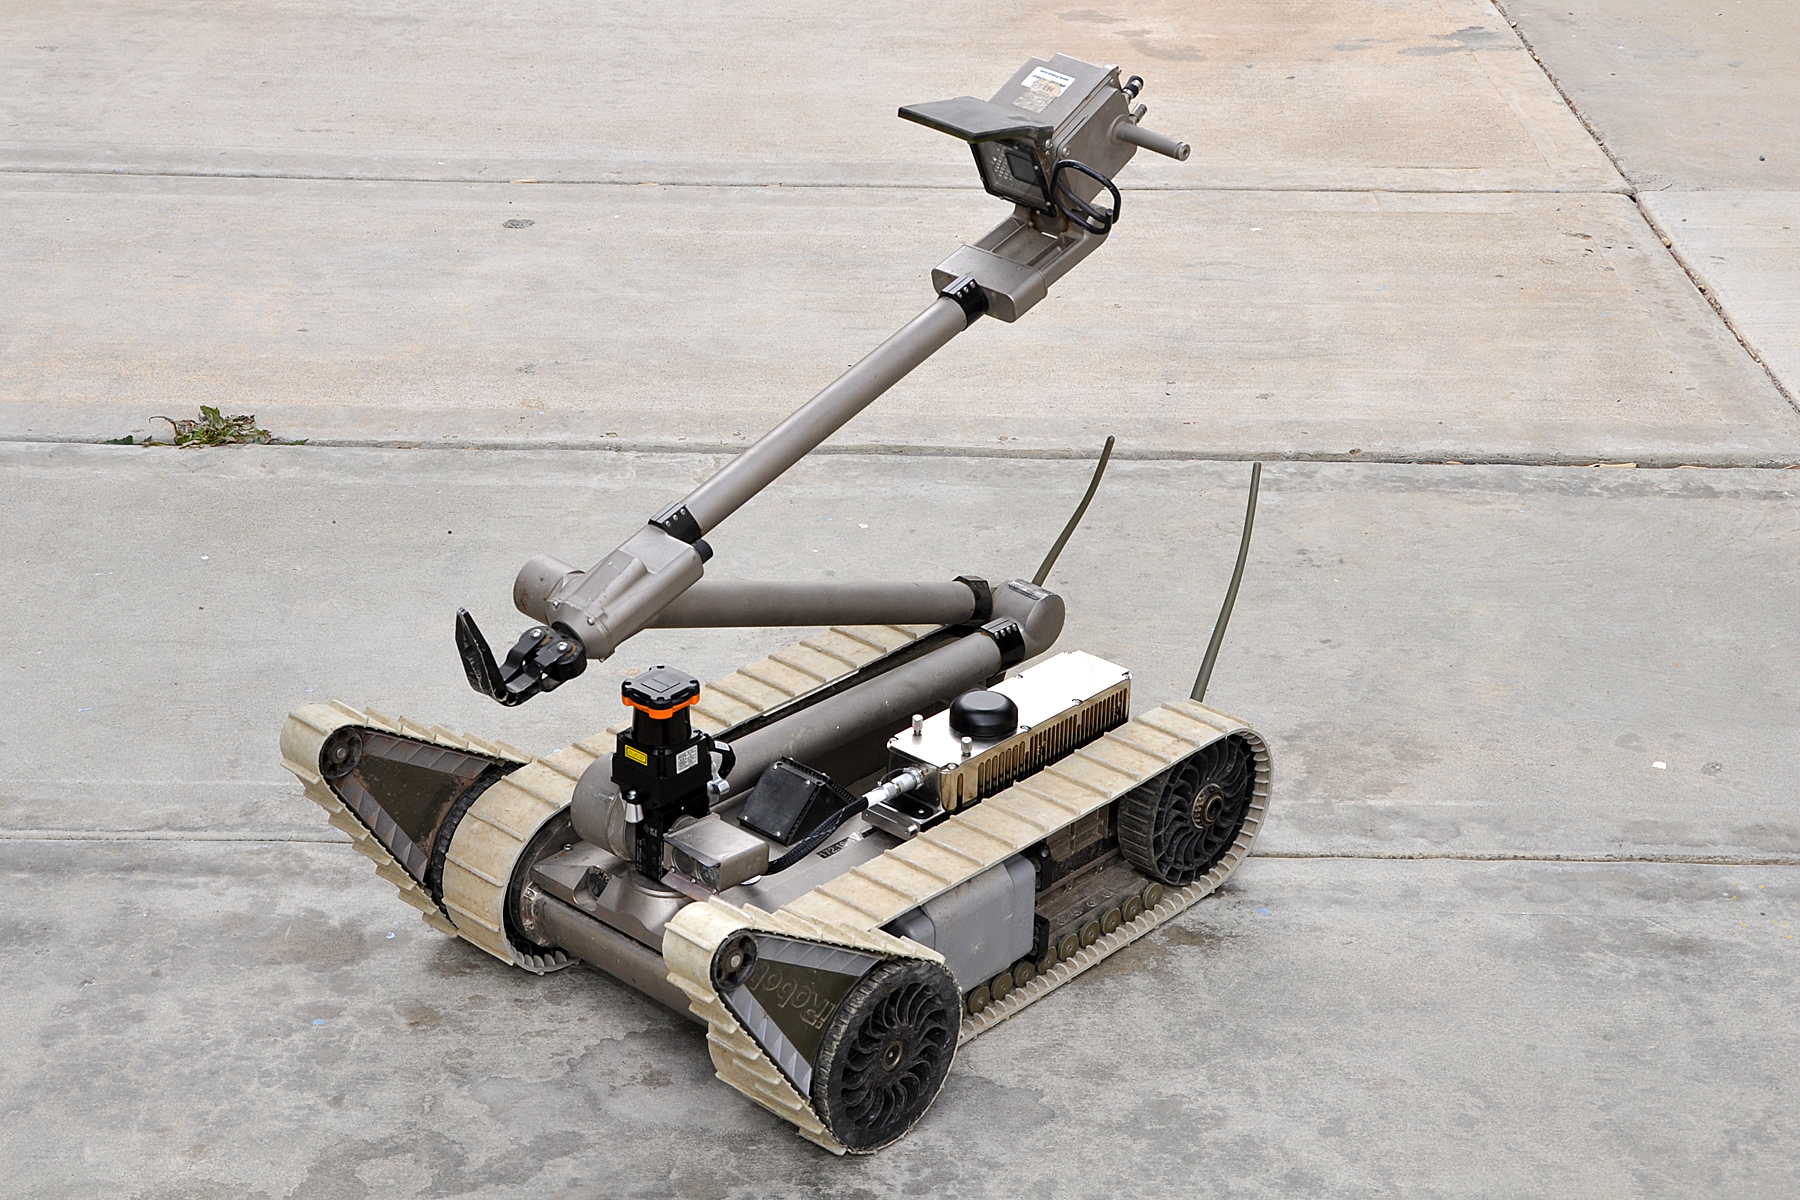
\includegraphics[width=.3\textwidth]{images/packbotRetrotraverse}
	\caption{iRobot Packbot}
	\label{fig:packbot}
\end{figure}

The \href{http://www.foster-miller.com/lemming.htm}{Talon} is manufactured by Foster Miller and is shown in Figure \ref{fig:talon}.

\begin{figure}[ht!]
	\centering
	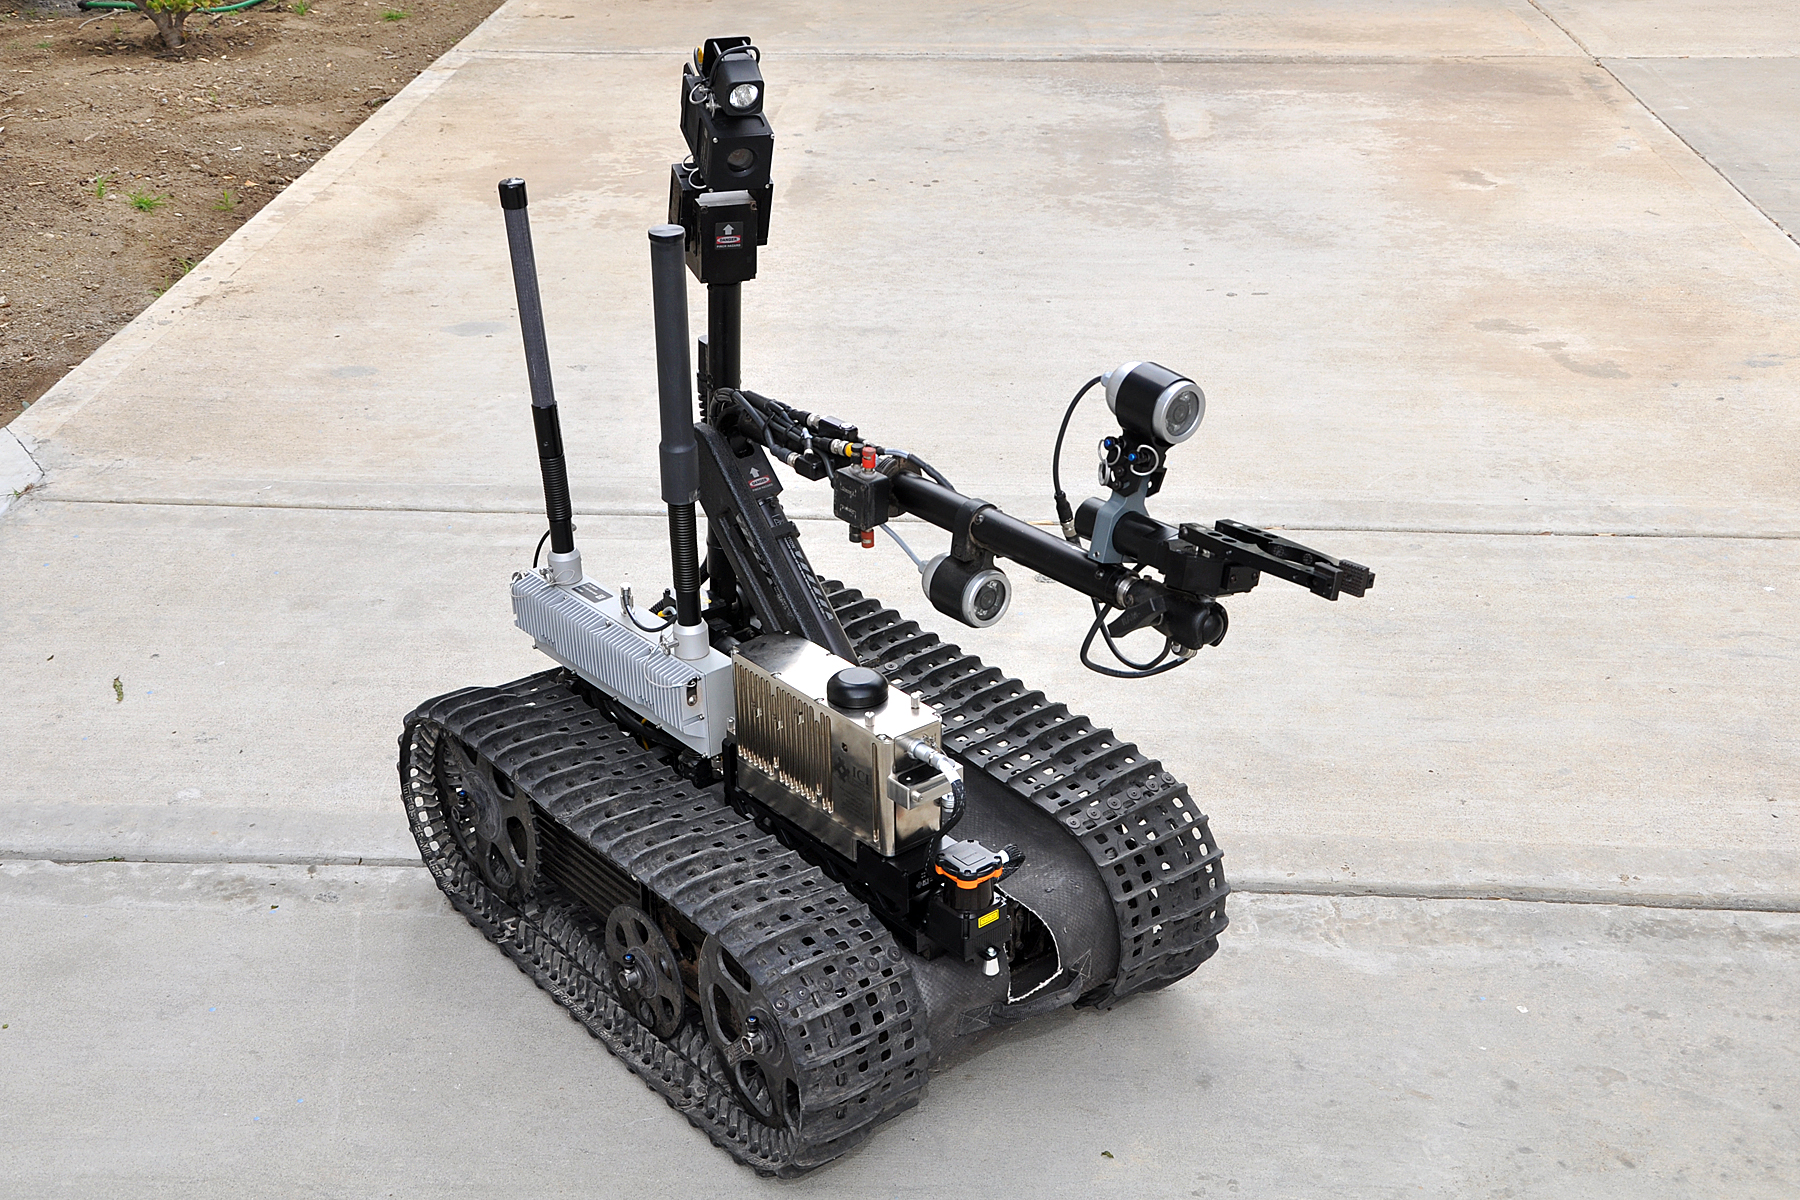
\includegraphics[width=.3\textwidth]{images/talonRetrotraverse}
	\caption{Foster Miller Talon}
	\label{fig:talon}
\end{figure}

The \href{http://www.spawar.navy.mil/robots/land/mprs/mprs.html}{Urbot} is an experimental prototype of a small UGV developed by SSCPAC and is shown in Figure \ref{fig:urbot}.

\begin{figure}[ht!]
	\centering
	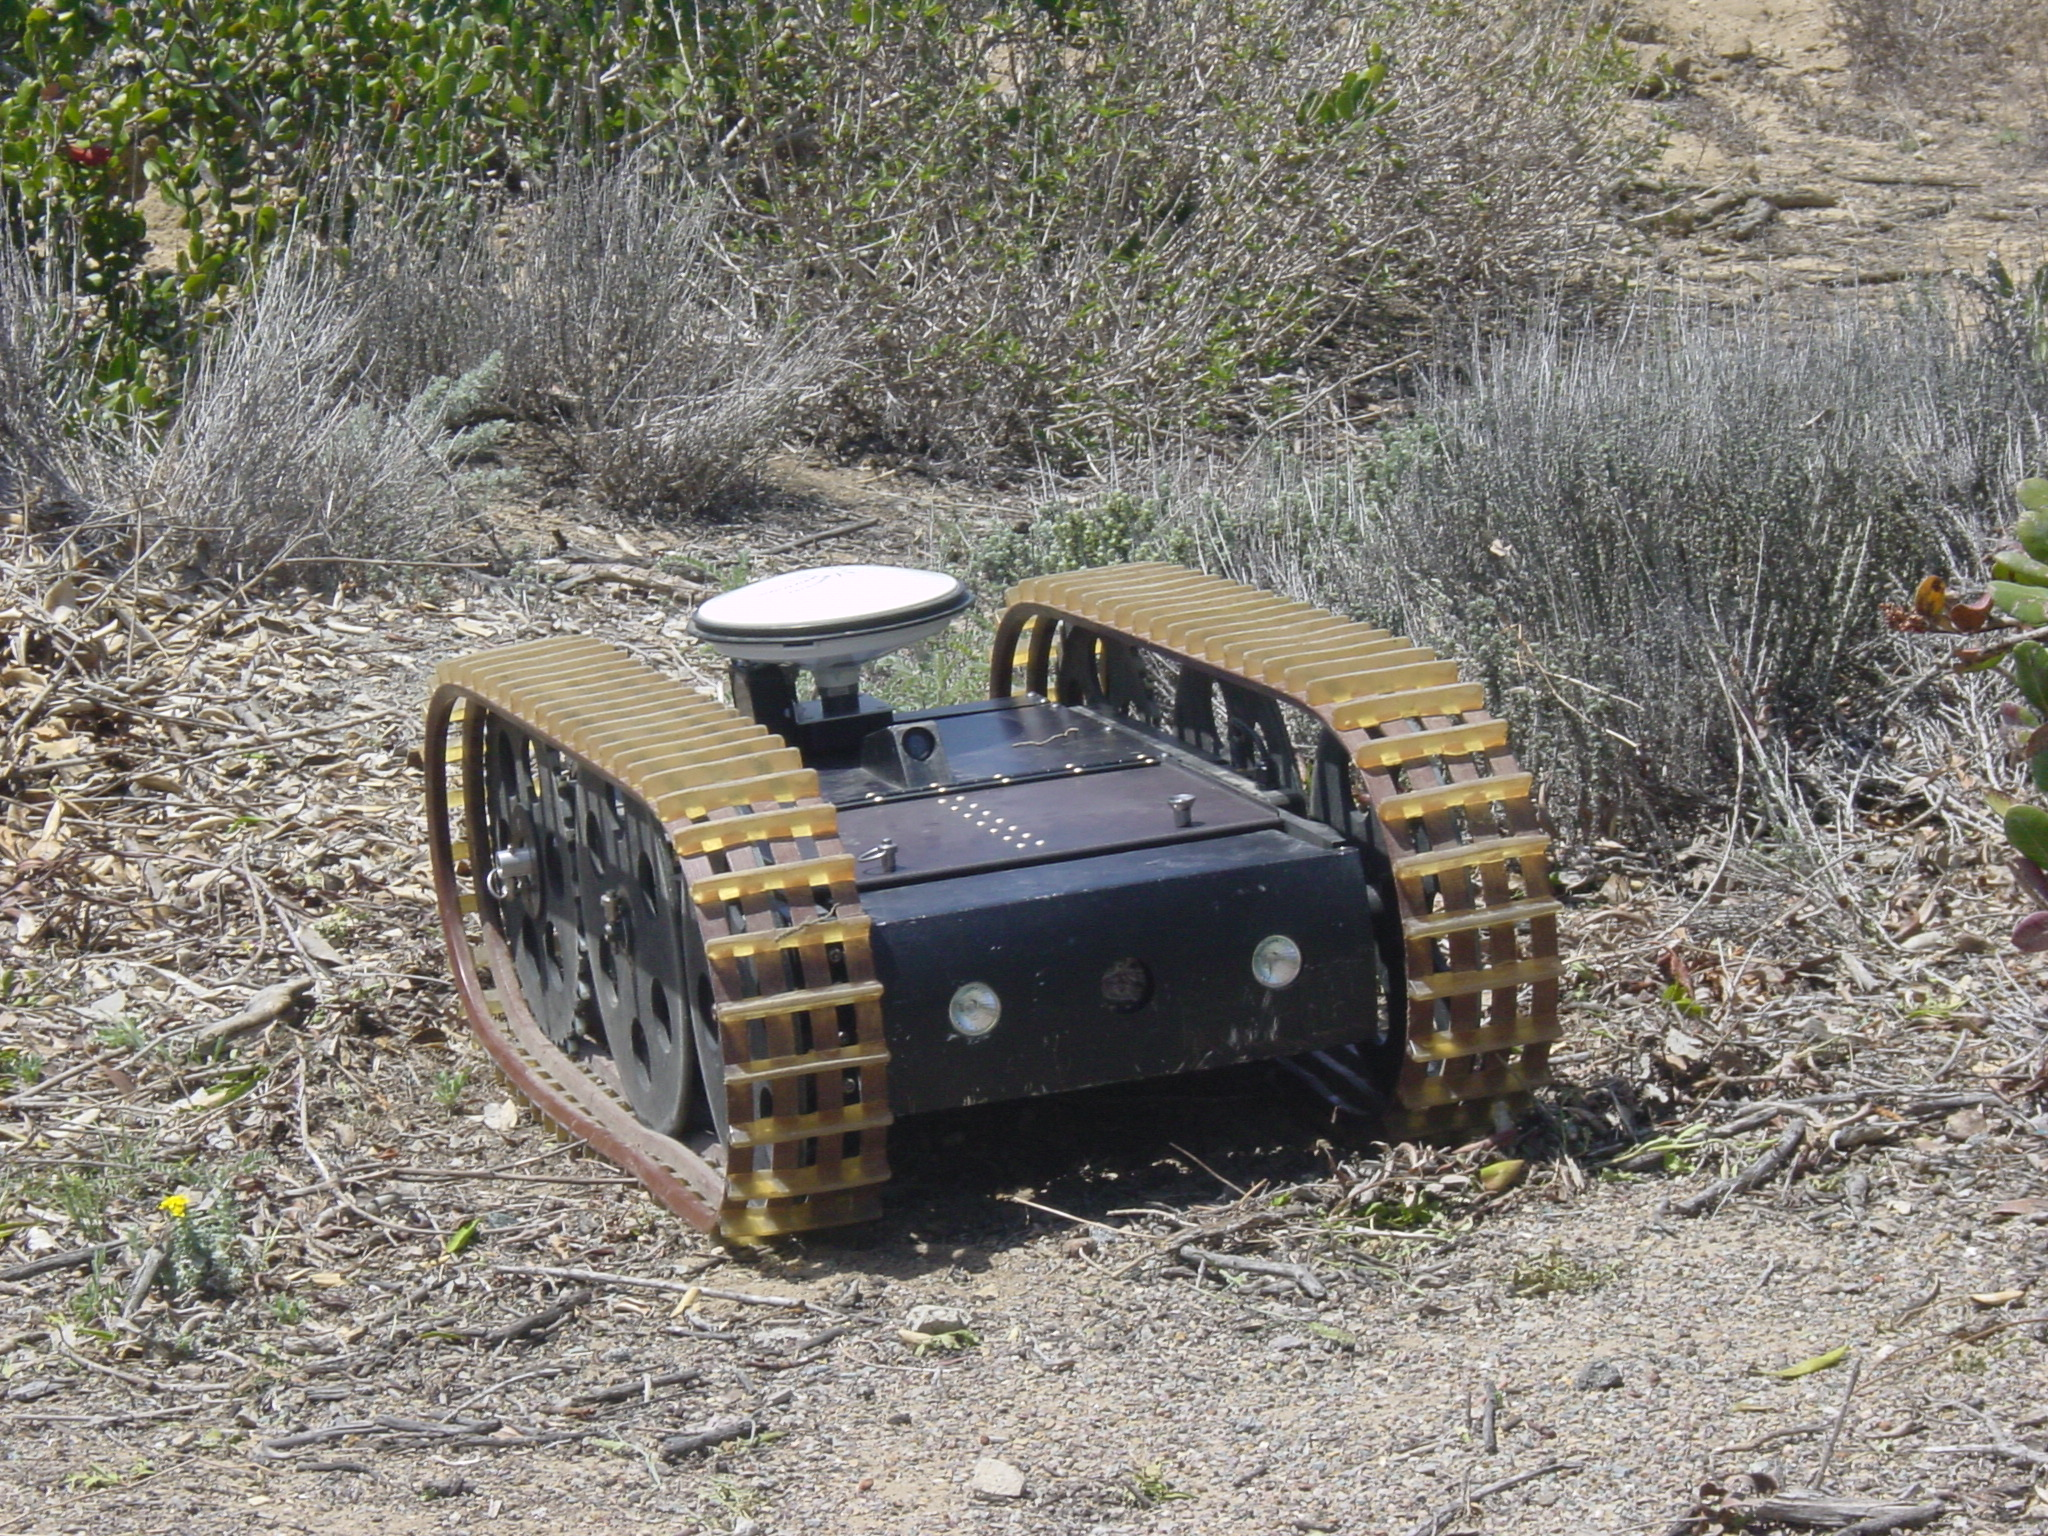
\includegraphics[width=.3\textwidth]{images/urbotWithGps}
	\caption{SSCPAC Urbot}
	\label{fig:urbot}
\end{figure}

\section{MOCU \& JAUS}
\label{sec:mocujaus}
The Multi-Robot Operator Control Unit (MOCU) in Figure \ref{fig:mocu} is a highly configurable front-end for simultaneous command and control of multiple systems and was created at SSCPAC \cite{PowellMOCU08}. MOCU has the ability to use a variety of communications protocols for interfacing to different systems and uses the Joint Architecture for Unmanned Systems (JAUS) protocol to send and receive data to all of the UGVs used in this research \cite{RoweJAUS08}. A combination of teleoperation using a joystick controller and autonomous navigation were used to collect data and test new ideas for estimation and controls. From within MOCU waypoints can be drawn on the overhead image and from those waypoints a route is generated and uploaded to the robot using the JAUS protocol. The robot will then attempt to drive that route autonomously and send back status information to MOCU using the controls and estimation code that is the focus of this research.

\begin{figure}[ht!]
	\centering
	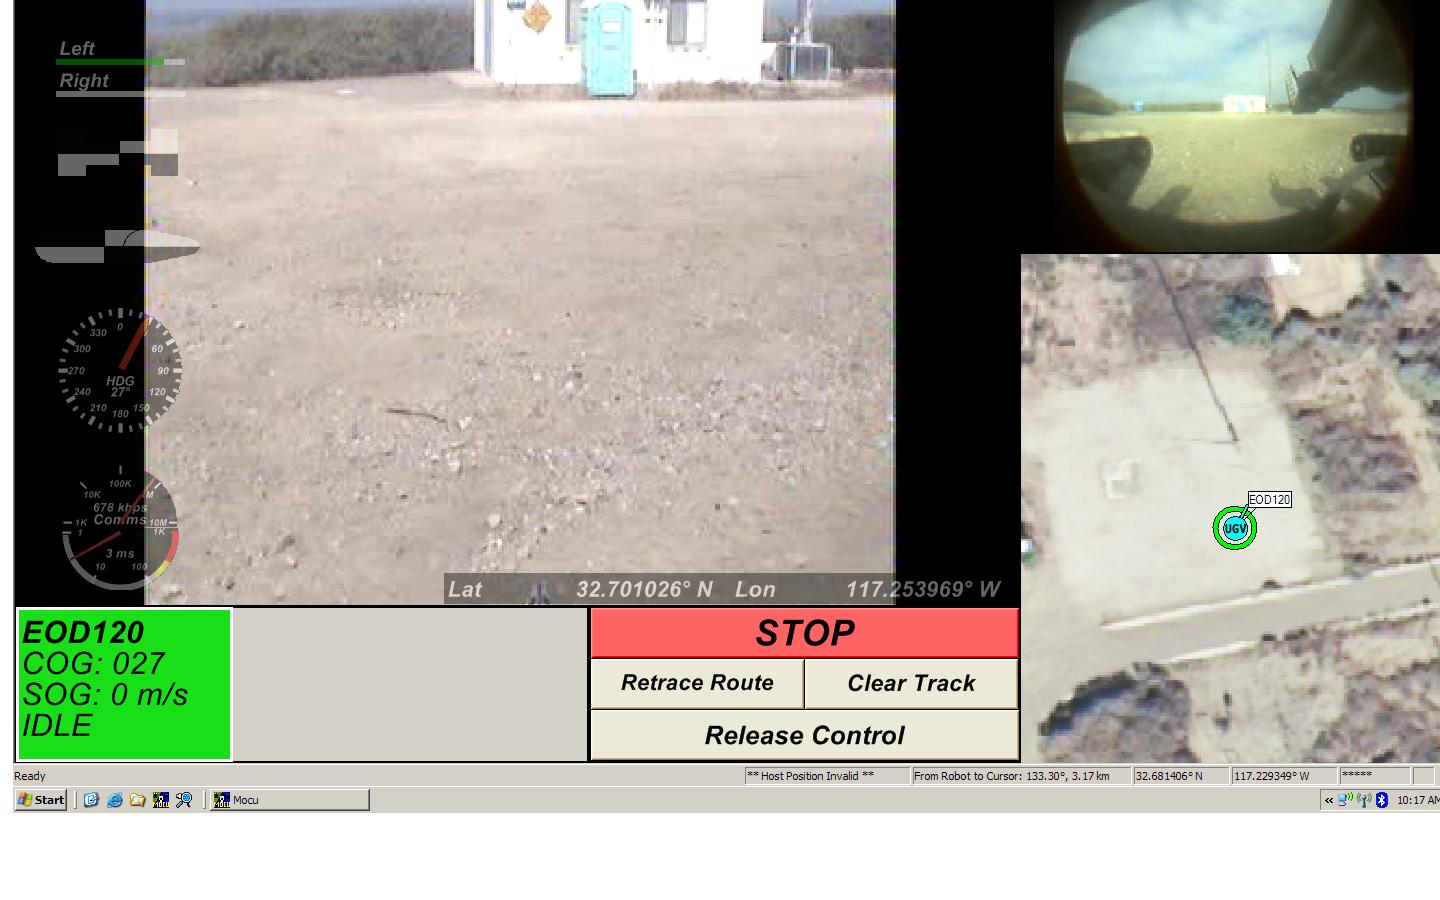
\includegraphics[width=.75\textwidth]{images/mocuPackbotScreenshot}
	\caption{Controlling PackBot with MOCU}
	\label{fig:mocu}
\end{figure}

\section{The Duals: Estimation \& Controls}
\label{sec:duals}
It is very difficult to simply work on either state estimation or controls individually as there is a large amount of coupling between the two areas. Although the main goal is to make the robots drive more smoothly and the actuator and motor outputs are ultimately generated by the control system it is still the case that the role of state estimation is equally important. If there exist large meaurement errors, drift or bias in the sensor readings then the robot will not have a very good idea of where it is locted and there will not be a controller that can stabilize the system.

An example would be when the only sensor available for measurements is an IMU which suffers from drift and bias, where both effects are exagerrated by temperature. There have been situations in which an IMU was in a robot with the motors turned off so that the robot is not moving. However, due to excessive heat in the electronics box the IMU measurements report that the heading of the robot keeps moving in circles at a rate of $\frac{\pi}{5} rad/s$. With a controller that was known to keep the robot stable when the IMU was working properly started forcing the robot to turn in circles when the motors were turned on even though the command was to stay in one place. This shows the importance of state estimation on overall robot performance -- it is not enough to only have a good controller. A perfect controller will follow noisy estimates exactly and result in erratic behavior. Conversely, a poor controller will not output smooth trajectories even given perfect state estimates.

\section{Sensors}
\label{sec:bgSensors}
The PackBot has its own computer that takes in commands for desired linear and angular velocities and outputs the correct motor controller commands. Typically the desired linear and angular velocity commands are generated by a user with a remote control. The research in this thesis used a set of sensors installed in one of the payload bays of the PackBot to determine which linear and angular velocity commands to send to the main PackBot computer without human intervention.

\subsection{Computer}
\label{sec:bgComputer}
The computer on the PackBot used for running the estimation and controls algorithms found in this thesis is the \href{http://www.beckhoff.com/english.asp?motherboards/cb4051.htm}{Beckhoff CB4051} with an Intel 2.0 GHz Core 2 Duo CPU.

\subsection{IMU}
\label{sec:bgIMU}
The IMU in the PackBot payload bay is a \href{http://www.microstrain.com/3dm-gx1.aspx}{Microstrain 3DM-GX1} that outputs Euler angles and angular rates.

\subsection{GPS}
\label{sec:bgGPS}
The GPS receiver in the PackBot payload by is a \href{http://www.novatel.com/products/gnss-receivers/oem-receiver-boards/oemv-receivers/}{Novatel OEMV}.

\subsection{Compass}
\label{sec:bgCompass}
Originally this sensor was not used on the PackBot but after initial testing it was determined that the heading reported by the Microstrain 3DM-GX1 was not very reliable and an \href{http://www.oceanserver-store.com/os3axdico3.html}{Ocean Server} compass was added to the PackBot payload bay.

\subsection{Wheel Encoders}
\label{sec:bgEncoders}
The PackBot is manufactured with wheel encoders that are read by the main PackBot computer and used to calculate a linear velocity and angular velocity that can be read by the payload computer when communicating with the main PackBot computer. Initially the wheel encoder data was not being used for backwards compatibility with other small UGVs that do not have wheel encoders but the systems that do not have wheel encoders are no longer used by EOD groups so that data has been incorporated into the sensor suite used by the algorithms in this thesis.

\section{Estimation and Control Software}
\label{sec:bgSoftware}
The SSCPAC robotics group has developed the Autonomous Capabilities Suite (ACS) which incorporates many different robotics related algorithms into a single software package that can be run on a wide variety of robots and is able to easily accomodate different payload and sensor suites \cite{Sights06}. The Kalman filter implementation was done in ACS.

A JAUS library written by SSCPAC provides for communications between the robots and MOCU.

The original path planning and controls software was written by SSCPAC for the Man Portable Robotic Systems (MPRS) program \cite{Bruch02} and extended for use on unmanned surface vehicles \cite{Ebken05, Larson06, Larson07}.

\chapter{State Estimation}
\label{ch:estimation}
The SSCPAC robotics group has developed the Autonomous Capabilities Suite (ACS) which incorporates many different robotics related algorithms into a single software package that can be run on a wide variety of robots and is able to easily accomodate different payload and sensor suites \cite{Sights06}. One of the ACS libraries is the adaptive extended Kalman filter which is used on the EOD robots for state estimation and is the main method used for answering the question ``Where am I?''. The idea behind the Kalman filter is relatively straightforward in that the robot has some basic idea of where it is in the world using its sensors but there is uncertainty involved in that estimate due to:
\begin{itemize}
\item different measurement accuracies from the sensors,
\item multiple sensors measuring the same state,
\item some states that are not measured,
\item imperfect models of the robot dynamics.
\end{itemize}

The Kalman filter is a method to merge physical models and sensor data to come up with a better estimate of where the robot is located, what its orientation is and how fast it is moving than any of the sensors measure on their own. There are four models used in the Kalman filter:
\begin{itemize}
\item system model based on physics,
\item measurement model to transform sensor output to state coordinate system,
\item system noise model,
\item measurement noise model.
\end{itemize}

%*** Put in a picture of the PackBot driving with one track going over two-by-fours. ***

%*** May want to use the example from the KF presentation instead of this example. I could use better images that way as well. ***

%An example is trying to determine the heading of a robot that is driving in a straight line where the left track is moving on a flat surface while the right track is moving on an uneven surface as in Figure \ref{fig:topology}. The wheel encoders measure the distance traveled by each track and will report that the right track is traveling a greater distance than the left track which could mean that (a) the robot is turning counter-clockwise or (b) the robot tracks are moving over different surface topologies. At the same time the robot will be getting measurements about its heading from both the IMU and GPS sensors where each of those sensors will have some noise as well. As long as the controller is performing adequately and the robot is indeed traveling in a straight line with a constant heading then the IMU and GPS sensor measurements would likely indicate that the robot is traveling in a straight line. The job of the Kalman filter is to determine how much to trust the IMU, GPS and wheel encoders when calculating the robot heading and to give an accurate estimate of the actual state of the robot at any given time, especially in situations like this example where there are possible conflicting measurements.

%\begin{figure}[ht!]
%	\centering
%	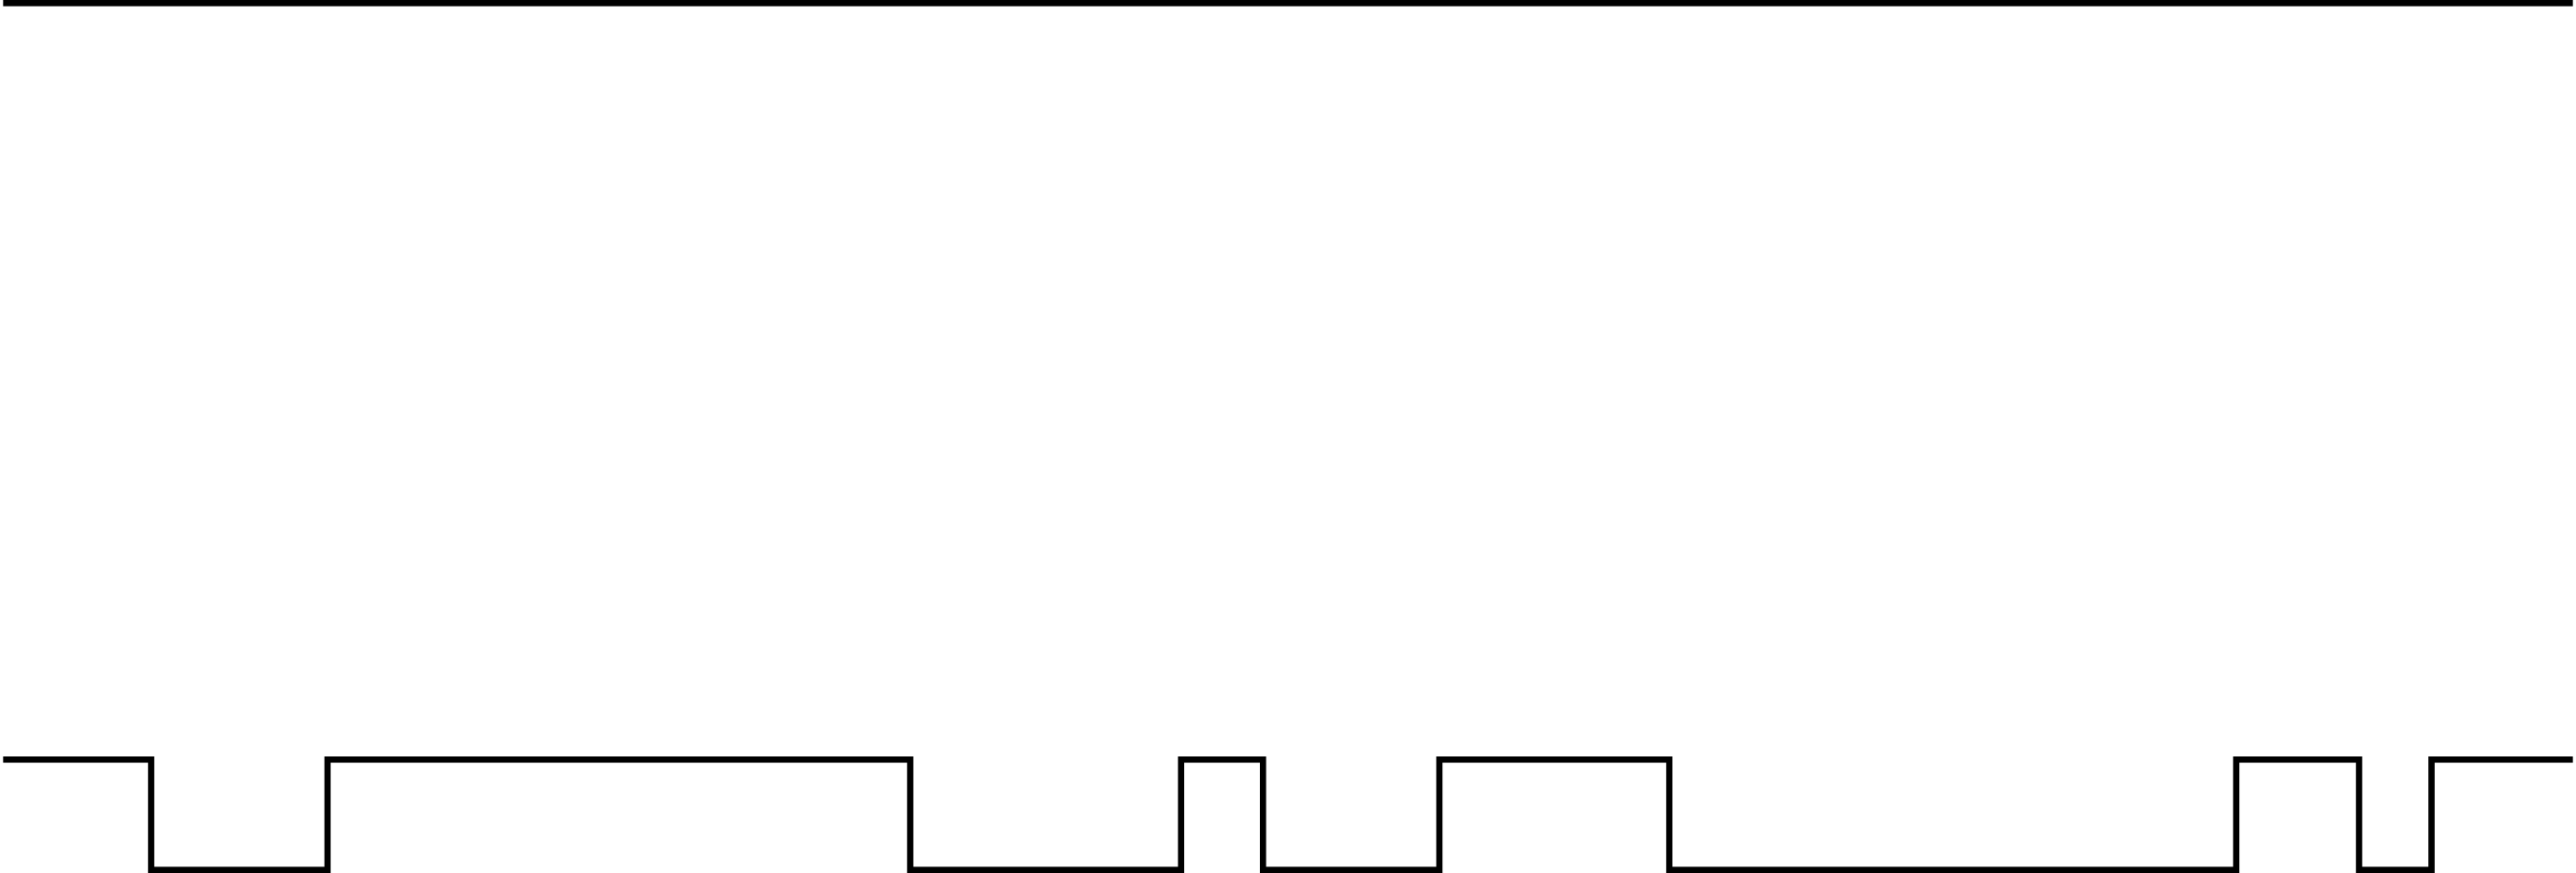
\includegraphics[width=.5\textwidth]{images/topography}
%	\caption{Different topologies for the left track and the right track when the ground is smooth on the left side and bumpy on the right side. The top line is for the left track and the bottom line is for the right track. The right track travels a greater distance than the left track.}
%	\label{fig:topology}
%\end{figure}

\section{State Space Models}
\label{sec:statespacemodels}
Kalman filters and modern control systems (see Chapter \ref{ch:controls}) use the idea of a multi-dimensional state space to encapsulate all of the relevant information that is known about a system. In the case of robots like the ones used in these experiments the states of interest are position, orientation and linear and angular velocities. In general a system is described by nonlinear equations that describe how the state variables change through time and how measurements of the system are related to the states as given by

\begin{align}
\label{eq:statespace}
\begin{split}
\dot{x} &= f(x,u,t) \\
\dot{y} &= h(x,t).
\end{split}
\end{align}

The state variables are given in vector form by $x$ and the sensor measurements are contained in the vector $y$. The state space equations are a means of representing with compact notations how the state of a system changes through time based on the initial state of the system and the inputs to the system, $u$, which allows the trajectory (or motion through time) to be calculated. The inputs are assumed to include any external forces applied to the system as well as actuation provided by the system itself. The function $h(x,t)$ transforms the sensor measurements into state variables which is important when the units of a sensor are not the same as the units of the state.

For the robots used in these experiments the state vector used follows that found in \cite{Kelly_1994_338}, \cite{Kelly_1994_333} where the state variables are

\begin{align*}
x_k = \left[\begin{array}{c c c c c c c c} x & y & z & V & \theta & \phi & \psi & \omega \end{array}\right]^T.
\end{align*}
In this vector $x$, $y$ and $z$ are positions, $V$ is linear velocity, $\theta$, $\phi$ and $\psi$ are Euler angles for pitch, roll and yaw, and $\omega$ is angular velocity as shown in Figure \ref{fig:packbotaxes}.

\begin{figure}[ht!]
    \centering
    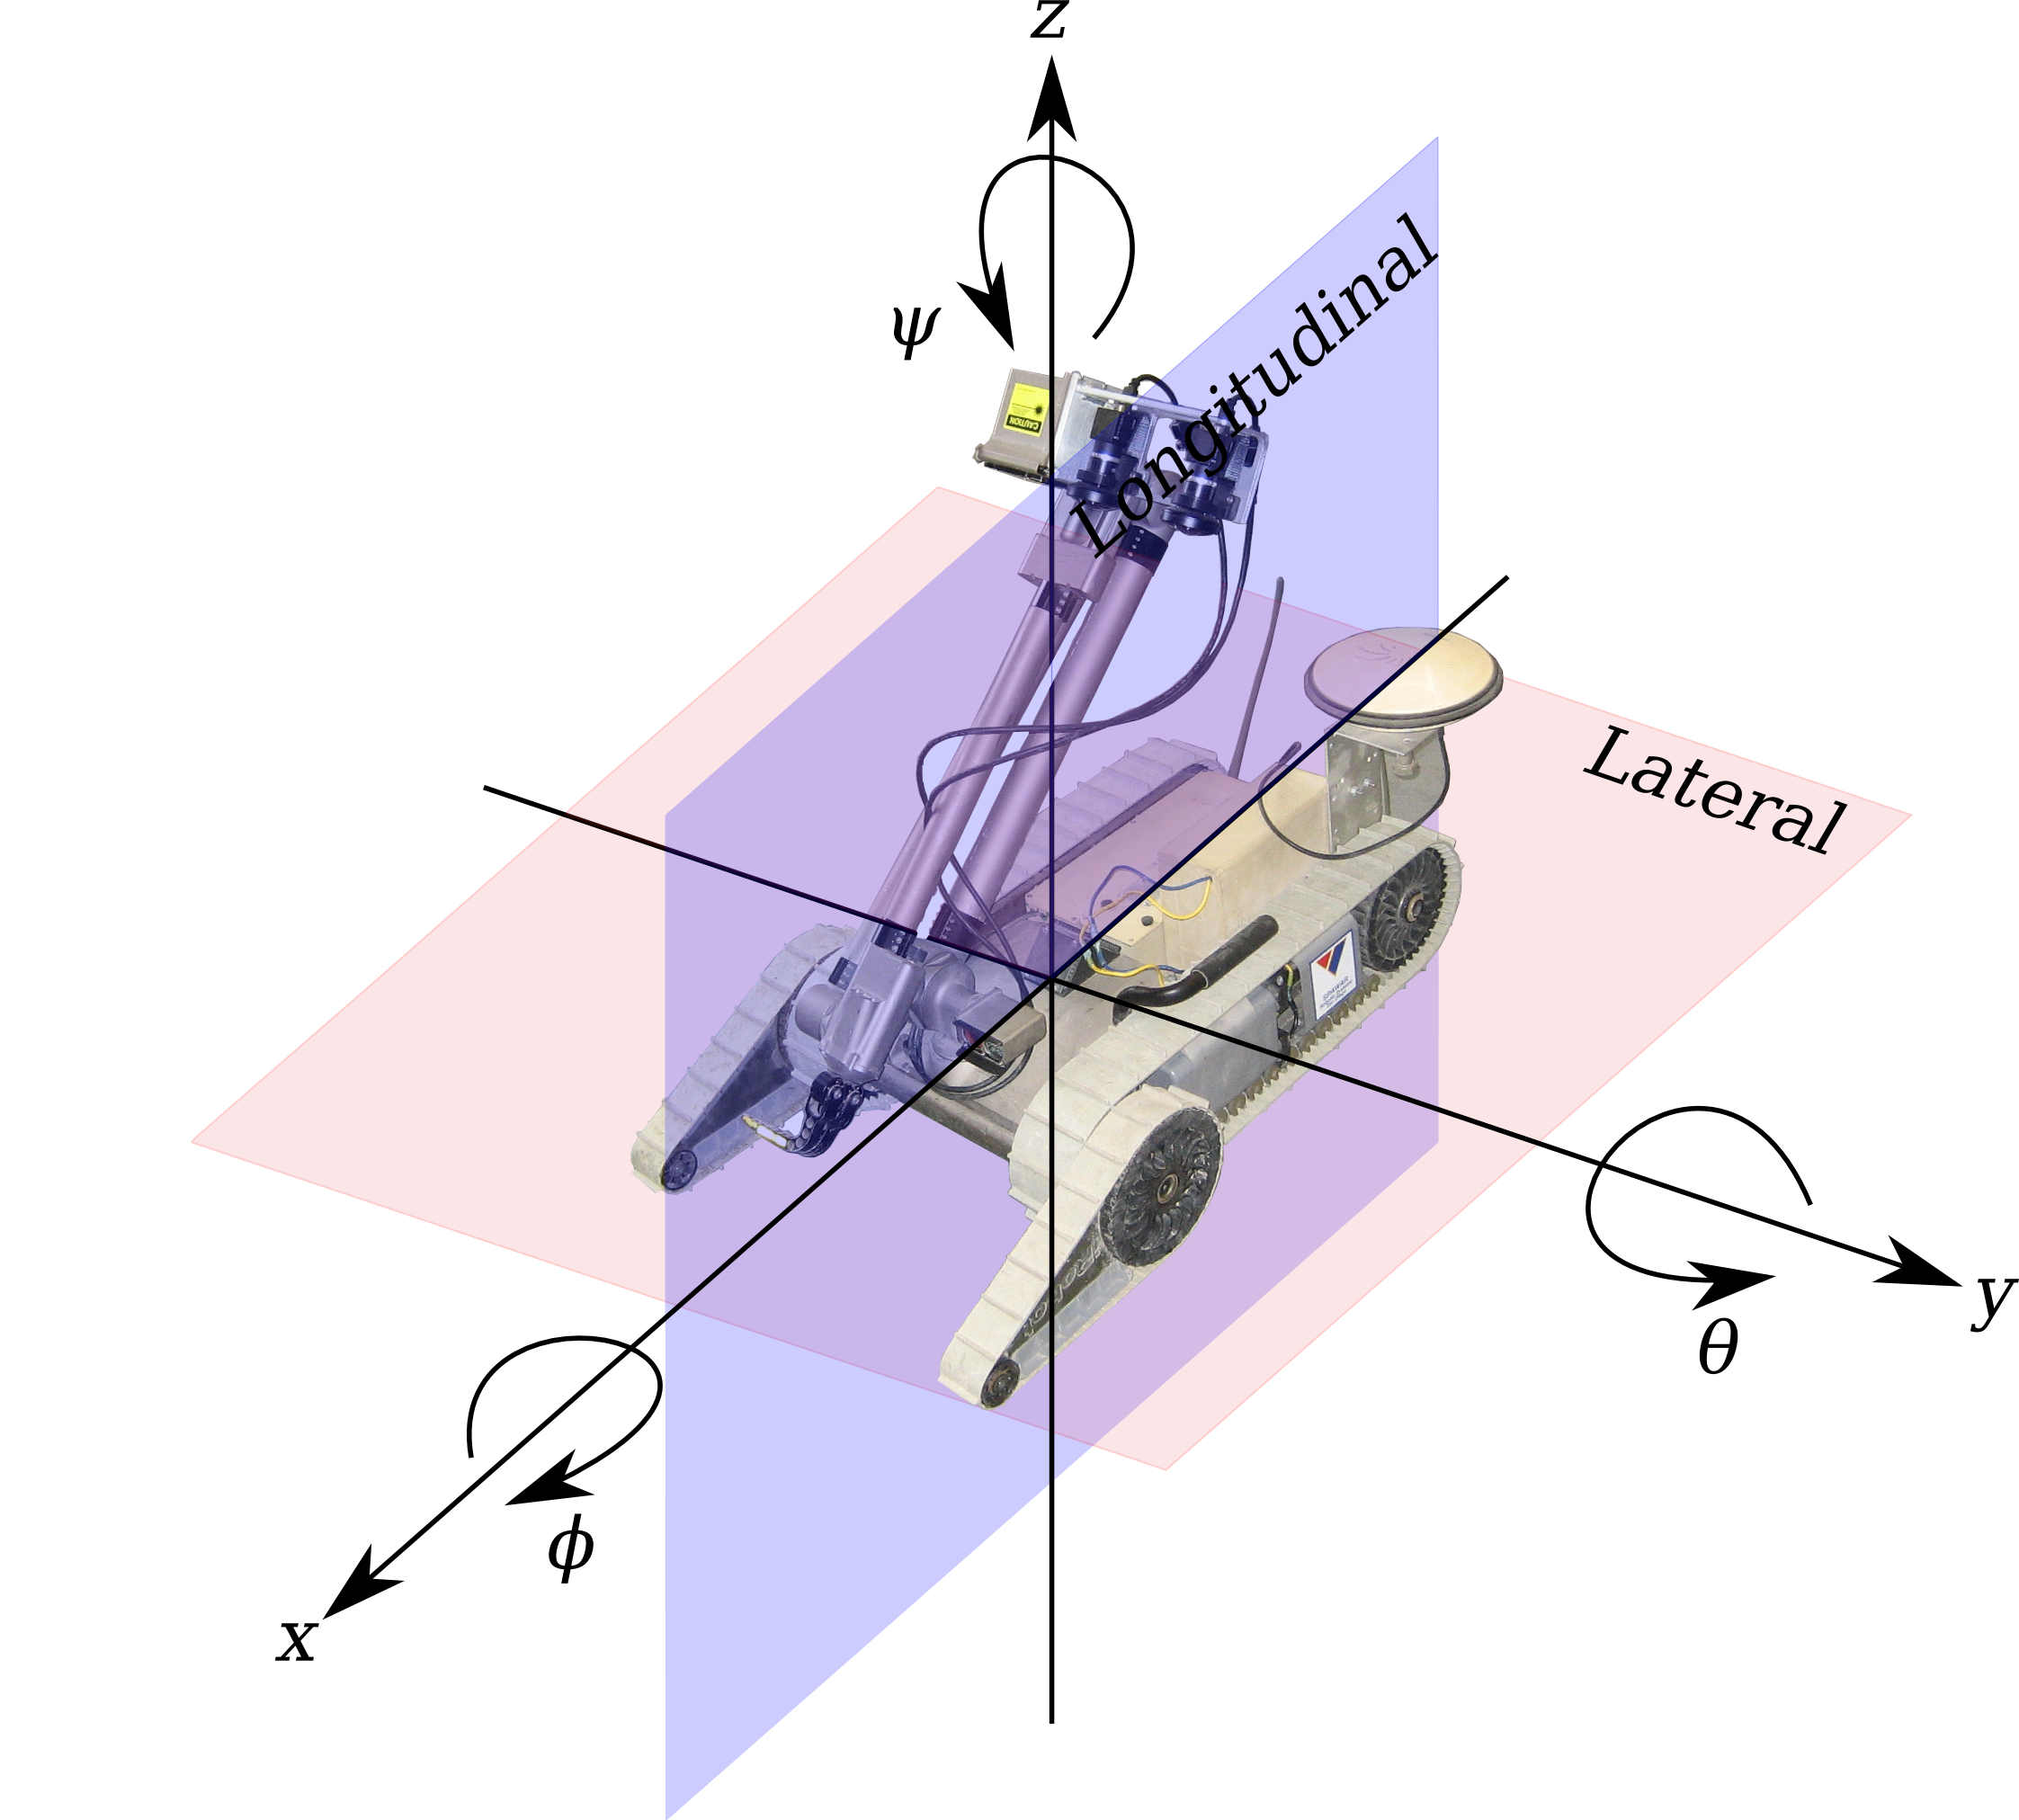
\includegraphics[width=.8\textwidth]{images/packbotaxes}
    \caption{PackBot used in experiments with axes for position and orientation shown.}
    \label{fig:packbotaxes}
\end{figure}

\section{The Kalman Filter}
\label{sec:kalmanfilter}
The ACS Kalman filter is typical of all Kalman filters in that it consists of a prediction update step and a measurement update step where the prediction update is run as fast as possible and the measurement update is run whenever new sensor data becomes available as in Figure \ref{fig:kf}. The prediction update step uses a model of the system dynamics and a measurement of elapsed time to determine where the system is in the world and will inevitably have errors. Some of the errors are due to effects that are not captured in the models, (im)precision of the clock on the computer for measuring time and simplifying assumptions that are made in order to be able to calculate the system model in real-time using embedded computers. The measurement update step is basically a feedback step to help correct for errors in the system model using sensors to provide current data \cite{Kelly_1994_338}.

\begin{figure}[ht!]
	\centering
	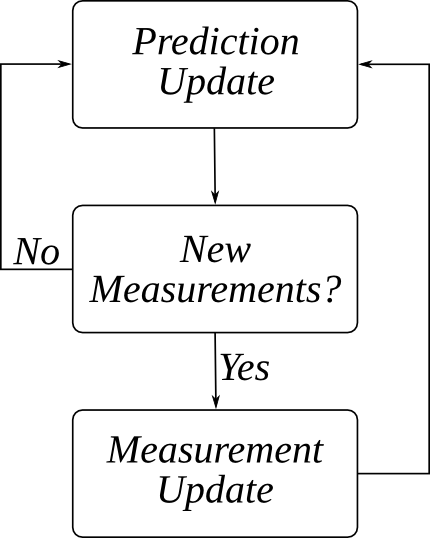
\includegraphics[width=.4\textwidth]{images/kf}
	\caption{The Kalman filter algorithm.}
	\label{fig:kf}
\end{figure}

The Kalman filters that run on the small UGVs used in these experiments run on digital computers and are necessarily used in discrete time rather than continuous time because of the nature of computers. Additionally, the standard Kalman filter equations make the assumption that the system and measurement models are linear. From \cite{Kelly_1994_338}, \cite{Simon06OptimalEstimation} the discretized and linearized versions of (\ref{eq:statespace}) mean that the state space equations are represented as

\begin{align}
\label{eq:kfstatemodel}
\begin{split}
x_{k+1} &= \Phi_kx_k + w_k \\
y_k &= H_kx_k + v_k
\end{split}
\end{align}
where $\Phi_k$ is the state transition matrix relating the state at time $k+1$ to time $k$ in the absence of inputs or noise and models the system dynamics, $w_k$ is system noise due to an imperfect model, $H_k$ is the measurement matrix which relates the measurements to the state vector and $v_k$ is the sensor measurement noise. The Kalman filter uses an unforced model so all inputs are considered disturbances to the steady-state dynamics. This means that $w_k$ includes noise, modeling errors, external forces and actuator forces.

The prediction update step marches the system dynamics forward in time using the equations

\begin{align}
\label{eq:kfpredictionupdate}
\begin{split}
\hat{x}_{k+1}^- &= \Phi_k\hat{x}_k^+ \\
P_{k+1}^- &= \Phi_kP_k^+\Phi_k^T + Q_k
\end{split}
\end{align}
and the measurement update step provides feedback from sensor data using the equations

\begin{align}
\label{eq:kfmeasurementupdate}
\begin{split}
K_k &= P_k^-H_k^T\left[H_kP_k^-H_k^T + R_k\right]^{-1} \\
\hat{x}_k^+ &= \hat{x}_k^- + K_k\left[y_k - H_k\hat{x}_k^-\right] \\
P_k^+ &= \left[I - K_kH_k\right]P_k^-.
\end{split}
\end{align}
where $P_k$ is the state covariance matrix, $K_k$ is the Kalman gain, $Q_k$ is the process covariance matrix giving a measure of the expected noise in the system model and $R_k$ is the measurement covariance matrix giving the expected noise of the sensors. Using (\ref{eq:kfpredictionupdate}) and (\ref{eq:kfmeasurementupdate}) an estimate of the state of the robot can be obtained at any time for use by the controls algorithms or to give feedback to a human operator.

*** Somewhere, maybe here, I want to say that $P_k$ is a measure of how good the state estimate is likely to be and that the gain $K_k$ weights whether the state estimate is based on the system model or the measurements. The gain $K_k$ is a function of the process and measurement covariance matrices so it really matters how those variances are set up relative to one another more than that they are absolutely correct values. ***

The variables $\hat{x}_k^-$ and $\hat{x}_k^+$ in (\ref{eq:kfpredictionupdate}) and (\ref{eq:kfmeasurementupdate}) refer to estimates of the state variables before and after the measurement update step in the Kalman filter, respectively.

\subsection{Models in the Kalman Filter}
\label{sec:kfModels}
The Kalman filter relies on several models that are used to determine estimates of the states for a system. The ACS Kalman filter uses four such models:

\begin{itemize}
\item System dynamics model,
\item measurement model,
\item system noise model,
\item measurement noise model.
\end{itemize}

It is important to recognize that the interaction between these four models determines how well the Kalman filter output will represent the true state of the robot.

\subsection{Assumptions in the System Model}
\label{sec:kfAssumptions}
It is nearly impossible to develop models that completely capture all of the attributes of most systems, including robots that are expected to operate in many different physical environments, so assumptions are made to simplify the system model. The following assumptions allow the prediction update step to be calculated in a reasonable amount of time using modern computers so that a state estimate is available that the control systems can act upon in real time. The assumptions also allow a single system model to be abstracted and used on multiple similar but different robotic vehicles.

\subsubsection{Low Dynamics Assumption}
\label{sec:kfLowDynamicsAssumption}
The first assumption made is that, from one time step to the next, the robot will not be accelerating fast enough in any direction for the sensors on the robot to be able to measure the accelerations. This means that the two velocities, linear and angular, in the state vector will be assumed to be constant. The benefit of this assumption is that there are six fewer states that must be tracked in the state vector, one for acceleration about each axis of the robot.

\subsubsection{Principal Motion Assumption}
\label{sec:kfPrincipalMotionAssumption}
The second assumption says that, during a single time step, the position of the robot will only be a function of linear velocity and the orientation of the robot will only be a function of the angular velocity. Figure \ref{fig:packbotaxes} helps in visualizing the effect of rotating the robot about its center and how that will not affect the position of the robot. This assumption allows several terms in the system model to be set to zero.

\subsection{Continuous to Discrete Time Transform}
\label{sec:kfContToDiscTransform}
The system model will be developed using continuous time nonlinear differential equations but the Kalman filter on the robots will be running on digital computers so the model will need to be converted to discrete time. In continuous time the system model will be

\begin{align*}
\dot{x} = Fx
\end{align*}
and in discrete time the system model will be

\begin{align*}
x_{k+1} = \Phi_k x_k.
\end{align*}
The transformation from continuous to discrete time obeys an exponential matrix transformation with a Taylor series approximation *** reference??? *** given by

\begin{align*}
\Phi_k = e^{F\Delta_T} = I + F\Delta_T + \frac{(F\Delta_T)^2}{2!} + \ldots + \frac{(F\Delta_T)^n}{n!}
\end{align*}
Using the system model developed in (\ref{eq:kfjacobianresult}) *** not that equation but the linearized version with assumptions applied!!! *** the term $F^2=0$ so all of the higher order terms go to zero and the result is

\begin{align}
\label{eq:kfContToDiscTransform}
\Phi_k = I + F\Delta_T
\end{align}

\subsection{System Dynamics Model}
\label{sec:dynamics}
A model of the system dynamics is necessary in order to propagate the state of the system forward in time in the absence of measurements. It is impossible to create a perfect model of the system and even a nearly perfect model of the system will likely be too complex to compute fast enough for it to be useful. The best result that is typically available is a model with a large amount of assumptions where the most important aspects of the dynamics are captured in the model.

A nonlinear, continuous time model based on robot kinematics is developed in the body frame coordinate system using the states from \S\ref{sec:statespacemodels} is given by

\begin{align}
\label{eq:kfnonlineardynamics}
\begin{split}
\frac{d}{dt}\left[\begin{array}{c}
x \\ y \\ z \\ V \\ \theta \\ \phi \\ \psi \\ \omega
\end{array}\right] =
\left[\begin{array}{c}
V\cos\psi\cos\theta \\
V\sin\psi\cos\theta \\
-V\sin\theta \\
0 \\
-\omega\sin\phi \\
\omega\tan\theta\cos\phi \\
\omega\cos\phi/\cos\theta \\
0
\end{array}\right].
\end{split}
\end{align}

\subsection{Extended Kalman Filter}
\label{sec:extendedkf}
The basic Kalman filter makes the assumption that both the system model contained in $\Phi_k$ and the measurement model in $H_k$ are linear. The extended Kalman filter (EKF) allows for nonlinear models such as that given by (\ref{eq:kfnonlineardynamics}) to be used for $\Phi_k$, $H_k$ or both by linearizing the models around the state estimate. To linearize the models the Jacobian, or matrix of partial derivatives, is taken about the estimated state. The idea of linearization of a nonlinear model is shown in Figure \ref{fig:KFLinearization} where the linearization can be seen to be more accurate when the system nonlinearities are small meaning that the dynamics are slow.

\begin{figure}[ht!]
	\centering
    \subfloat[Slow dynamics.] {
	    \label{images/KFLinearizationSlow}
        \includegraphics[width=.3\textwidth]{images/KFLinearizationSlow}
    }
    \hfill
    \subfloat[Medium dynamics.] {
        \label{images/KFLinearizationMedium}
	    \includegraphics[width=.3\textwidth]{images/KFLinearizationMedium}
    }
    \hfill
    \subfloat[Fast dynamics.] {
        \label{images/KFLinearizationFast}
	    \includegraphics[width=.3\textwidth]{images/KFLinearizationFast}
    }
	\caption{Effects of linearizing a nonlinear model. Success depends on the speed of the dynamics, either \subref{images/KFLinearizationSlow} slow, \subref{images/KFLinearizationMedium} medium or \subref{images/KFLinearizationFast} fast.}
	\label{fig:KFLinearization}
\end{figure}

The nonlinear state dynamics were described in (\ref{eq:kfnonlineardynamics}). The Jacobian of that state vector equation is calculated using

%{\tiny
\begin{align*}
\dot{x} =
\underbrace{\left[\begin{array}{c c c c c c c c}
\frac{\partial \dot{x}}{\partial x} & \frac{\partial \dot{x}}{\partial y} & \frac{\partial \dot{x}}{\partial z} & \frac{\partial \dot{x}}{\partial V} & \frac{\partial \dot{x}}{\partial \theta} & \frac{\partial \dot{x}}{\partial \phi} & \frac{\partial \dot{x}}{\partial \psi} & \frac{\partial \dot{x}}{\partial \omega} \\
\frac{\partial \dot{y}}{\partial x} & \frac{\partial \dot{y}}{\partial y} & \frac{\partial \dot{y}}{\partial z} & \frac{\partial \dot{y}}{\partial V} & \frac{\partial \dot{y}}{\partial \theta} & \frac{\partial \dot{y}}{\partial \phi} & \frac{\partial \dot{y}}{\partial \psi} & \frac{\partial \dot{y}}{\partial \omega} \\
\frac{\partial \dot{z}}{\partial x} & \frac{\partial \dot{z}}{\partial y} & \frac{\partial \dot{z}}{\partial z} & \frac{\partial \dot{z}}{\partial V} & \frac{\partial \dot{z}}{\partial \theta} & \frac{\partial \dot{z}}{\partial \phi} & \frac{\partial \dot{z}}{\partial \psi} & \frac{\partial \dot{z}}{\partial \omega} \\
\frac{\partial \dot{V}}{\partial x} & \frac{\partial \dot{V}}{\partial y} & \frac{\partial \dot{V}}{\partial z} & \frac{\partial \dot{V}}{\partial V} & \frac{\partial \dot{V}}{\partial \theta} & \frac{\partial \dot{V}}{\partial \phi} & \frac{\partial \dot{V}}{\partial \psi} & \frac{\partial \dot{V}}{\partial \omega} \\
\frac{\partial \dot{\theta}}{\partial x} & \frac{\partial \dot{\theta}}{\partial y} & \frac{\partial \dot{\theta}}{\partial z} & \frac{\partial \dot{\theta}}{\partial V} & \frac{\partial \dot{\theta}}{\partial \theta} & \frac{\partial \dot{\theta}}{\partial \phi} & \frac{\partial \dot{\theta}}{\partial \psi} & \frac{\partial \dot{\theta}}{\partial \omega} \\
\frac{\partial \dot{\phi}}{\partial x} & \frac{\partial \dot{\phi}}{\partial y} & \frac{\partial \dot{\phi}}{\partial z} & \frac{\partial \dot{\phi}}{\partial V} & \frac{\partial \dot{\phi}}{\partial \theta} & \frac{\partial \dot{\phi}}{\partial \phi} & \frac{\partial \dot{\phi}}{\partial \psi} & \frac{\partial \dot{\phi}}{\partial \omega} \\
\frac{\partial \dot{\psi}}{\partial x} & \frac{\partial \dot{\psi}}{\partial y} & \frac{\partial \dot{\psi}}{\partial z} & \frac{\partial \dot{\psi}}{\partial V} & \frac{\partial \dot{\psi}}{\partial \theta} & \frac{\partial \dot{\psi}}{\partial \phi} & \frac{\partial \dot{\psi}}{\partial \psi} & \frac{\partial \dot{\psi}}{\partial \omega} \\
\frac{\partial \dot{\omega}}{\partial x} & \frac{\partial \dot{\omega}}{\partial y} & \frac{\partial \dot{\omega}}{\partial z} & \frac{\partial \dot{\omega}}{\partial V} & \frac{\partial \dot{\omega}}{\partial \theta} & \frac{\partial \dot{\omega}}{\partial \phi} & \frac{\partial \dot{\omega}}{\partial \psi} & \frac{\partial \dot{\omega}}{\partial \omega}
\end{array}\right]}_{F}
\left[\begin{array}{c}
x \\ y \\ z \\ V \\ \theta \\ \phi \\ \psi \\ \omega
\end{array}\right]
\end{align*}
%}
which results in

{\scriptsize
\begin{align}
\label{eq:kfjacobianresult}
\frac{d}{dt}\left[\begin{array}{c}
x \\ y \\ z \\ V \\ \theta \\ \phi \\ \psi \\ \omega
\end{array}\right] =
\underbrace{\left[\begin{array}{c c c c c c c c}
0 & 0 & 0 & c\psi c\theta & -V c\psi s\theta               & 0                     & -V s\psi c\theta & 0 \\
0 & 0 & 0 & s\psi c\theta & -V s\psi s\theta               & 0                     & V c\psi c\theta  & 0 \\
0 & 0 & 0 & -s\theta      & -V c\theta                     & 0                     & 0                & 0 \\
0 & 0 & 0 & 0             & 0                              & 0                     & 0                & 0 \\
0 & 0 & 0 & 0             & 0                              & -\omega c\phi         & 0                & -s\phi \\
0 & 0 & 0 & 0             & \omega c\phi/c^2\theta         & \omega t\theta s\phi  & 0                & t\theta c\phi \\
0 & 0 & 0 & 0             & \omega s\theta c\phi/c^2\theta & -\omega s\phi/c\theta & 0                & c\phi/c\theta \\
0 & 0 & 0 & 0             & 0                              & 0                     & 0                & 0
\end{array}\right]}_{F}
\left[\begin{array}{c}
x \\ y \\ z \\ V \\ \theta \\ \phi \\ \psi \\ \omega
\end{array}\right].
\end{align}
}
Applying the principal motion assumption to set the terms relating position and angular velocity as well as orientation and linear velocity to zero in addition to converting from continuous to discrete time to put ones on the diagonal gives

\begin{align}
\label{eq:kfSystemModelWithAssumptions}
x_{k+1} = 
\underbrace{\left[\begin{array}{c c c c c c c c}
1 & 0 & 0 & c\psi c\theta \Delta_T & 0 & 0 & 0 & 0 \\
0 & 1 & 0 & s\psi c\theta \Delta_T & 0 & 0 & 0 & 0\\
0 & 0 & 1 & -s\theta \Delta_T & 0 & 0 & 0 & 0\\
0 & 0 & 0 & 1 & 0 & 0 & 0 & 0 \\
0 & 0 & 0 & 0 & 1 & 0 & 0 & -s\phi \Delta_T \\
0 & 0 & 0 & 0 & 0 & 1 & 0 & t\theta c\phi \Delta_T \\
0 & 0 & 0 & 0 & 0 & 0 & 1 & c\phi \Delta_T/c\theta \\
0 & 0 & 0 & 0 & 0 & 0 & 0 & 1
\end{array}\right]}_{\Phi_k}
\left[\begin{array}{c}
x \\ y \\ z \\ V \\ \theta \\ \phi \\ \psi \\ \omega
\end{array}\right]_k
\end{align}
This is the system model that is used in the prediction update step of the Kalman filter equations to calculate the state of the robot in between measurements.

\subsection{Measurement Model}
\label{sec:kfMeasurementModel}

\subsection{Noise Models}
\label{sec:kfNoiseModels}

\subsection{Kalman Gain}
\label{kfKalmanGain}

\section{Establishing Ground Truth}
\label{sec:groundtruth}
Quantitatively evaluating the performance of Kalman filters can be accomplished in several ways, the best of which is to analyze the output of the Kalman filter against ground truth. Although it is nearly impossible to establish ground truth over a large area in practice the closer the measurements are to an absolute position in the world the better. To determine ground truth for the robots in these experiments a differential GPS (DGPS) system was created independently of the sensors on the robot so that very accurate measurements of the robots actual position could be logged and then used in a post-processing step to determine how well the Kalman filter estimate corresponds to ground truth.

The DGPS system consists of a GPS receiver and serial radio that make up the base station and a GPS receiver, serial radio and small computer that make up the roaming station as in Figure \ref{fig:dgps}. The GPS receivers are both Novatel receivers using the Real Time Kinematics algorithm. The base station is located in a static position and is configured to use a fixed position which is compared to what the current position would be if it were not fixed. The difference between the fixed position and the calculated position are used to generate corrections that would put the position of the GPS antenna at the fixed position and those corrections are sent to and applied at the roaming station resulting in a standard deviation of $2$ $cm$ for the position output of the roaming station. The errors are due to the effects of the GPS signal passing through the atmosphere from the satellites to the antenna as well as to multipath effects closer to the ground. The DGPS corrections are used for each satellite that the ground station and the roaming station share in the constellation of satellites they are using in their solution of a position estimate. The DGPS system is bootstrapped to the robot during testing runs to log data at a rate of $20$ $Hz$ and is only used as a tool to improve Kalman filter performance and is not meant to be used during normal operation.

With a highly accurate estimate of ground truth established it becomes possible to not only study the performance of the Kalman filter but to also begin determining whether to focus efforts in improving the autonomous navigation behaviors of the robots via the estimation or controls algorithms.

\begin{figure}[ht!]
	\centering
	\includegraphics[width=.6\textwidth]{images/dgps}
	\caption{Differential GPS system diagram.}
	\label{fig:dgps}
\end{figure}

\section{Identifying Noise Models}

\subsection{Adaptive Extended Kalman Filter}
\label{sec:adaptiveekf}
*** Discuss why $Q$ and $R$ are important and what function they serve in the Kalman filter. Why is it valid to update $Q$ and $R$ this way? Talk about how the updates are turned off when the velocity is zero, otherwise $Q$ and $R$ are adapted to a static, not dynamic, state. Similarly, talk about how this method doesn't work as well as would be hoped because the original application was for tracking satellites with low dynamics and robots have high dynamics, especially when navigating around obstacles. Also, look at the extra stuff that Busse says he had to do to get this algorithm to work in practice. I say high dynamics here, but what about the low dynamics assumption? Low is relative to sensor noise and satellites have much higher quality sensors so the noise level is much lower in addition to the actual dynamics being lower. ***

Attempting to determine the proper values for the covariance matrices $Q$ in (\ref{eq:kfpredictionupdate}) and $R$ in (\ref{eq:kfmeasurementupdate}) can be a laborious process and is often considered more of an art than a science with engineer experience being a critical factor. The ACS Kalman filter has been implemented with an adaptive scheme to update the covariance matrices in real time as the robot moves around and sensor measurements are taken into account to help overcome the time intensive nature of determining these matrices and add a degree of robustness to the state estimate \cite{Sights06}, \cite{Mehra72}, \cite{Busse03adaptiveEKF}. Estimates of $Q$ and $R$ are updated at alternating time steps in the EKF. Recall from (\ref{eq:kfpredictionupdate}) and (\ref{eq:kfmeasurementupdate}) that $\hat{x}_k^+$ and $P_k^+$ are known after the measurement update step and $\hat{x}_k^-$ and $P_k^-$ are known after the system update step in the Kalman filter.

As shown in \cite{Busse03adaptiveEKF} the first step is to calculate $Q^\star$ using

\begin{align*}
% \label{eq:qstar}
Q^\star = \left(\hat{x}_k^+-\hat{x}_k^-\right)\left(\hat{x}_k^+-\hat{x}_k^-\right)^T + P_k^- - P_k^+ - \hat{Q}_k^-.
\end{align*}
Then the estimate of $Q$ is updated such that

\begin{align}
\label{eq:qadapt}
\hat{Q}_k^+ = \hat{Q}_k^- + \frac{1}{L_Q}\left(Q^\star-\hat{Q}_k^-\right).
\end{align}

Next $R^\star$ is calculated using

\begin{align*}
% \label{eq:rstar}
R^\star = \left(y_k-\hat{y}_k^+\right)\left(y_k-\hat{y}_k^+\right)^T - H_kP_k^+H_k^T
\end{align*}
where $y_k$ are actual measurement data and $\hat{y}_k^+ = h_k\hat{x}_k^+$ is calculated after the measurement update step. Then the estimate of $R$ is updated such that

\begin{align}
\label{eq:radapt}
\hat{R}_k^+ = \hat{R}_k^- + \frac{1}{L_R}\left(R^\star-\hat{R}_k^-\right).
\end{align}

It can be seen that the estimates of both covariance matrices employ a running average algorithm and vary the weight of recent measurements and state updates via the adaptation coefficients $L_Q$ and $L_R$. *** Give example here? Explain more? Maybe, but only if I really start to compare it to the learned parameters and want to give a sense of what the differences are between the two methods. ***

\subsection{Discriminative Training of Kalman Filter Parameters}
\label{sec:trainingkfparams}
*** Investigate the difference between adaptive filtering and training. It seems like they accomplish the same thing, namely, convergence to some values for the covariance matrices. Do they use the same metrics? Do they converge to the same covariance matrices? Is it just online vs. offline training? Would a neural network be a good candidate for finding $Q$ and $R$ as well? All of these methods seem to be curve fitting in the multi-dimensional state space. Look at \S3.3 of \cite{Simon06OptimalEstimation} for details on how measurements affect state estimate via recursive least squares. I might also use \cite{Orderud05}. ***

\cite{Abbeel-RSS-05} describes a method to automatically learn what the covariance matrices $Q$ and $R$ should be that is an alternative, offline approach to the adaptive EKF from \S\ref{sec:adaptiveekf}. However, when used in conjunction with the adaptive EKF scheme this could allow for faster convergence times when the robots are started and for smaller ranges for the adaptation coefficients $L_Q$ and $L_R$ in (\ref{eq:qadapt}) and (\ref{eq:radapt}). This method takes advantage of ground truth measurements obtained using a DGPS system like that described in \S\ref{sec:groundtruth}. Note that in the following expressions the term $h(\mu_t)$ is the position output by the Kalman filter so that the goal is to find values of $Q$ and $R$ that cause the output of the Kalman filter to match ground truth as closely as possible.

The residual prediction error is used to estimate $Q$ and $R$ using

\begin{align*}
\left<R_{\text{res}},Q_{\text{res}}\right> = \argmin_{R,Q}\sum_{t=0}^T ||y_t-h(\mu_t)||_2^2.
\end{align*}
When the state covariance matrix $P$ is \textit{not} a multiple of the identity matrix $I$ then this metric is

\begin{align*}
\left<R_{\text{res}},Q_{\text{res}}\right> = \argmin_{R,Q}\sum_{t=0}^T (y_t-h(\mu_t))^TP^{-1}(y_t-h(\mu_t)).
\end{align*}
The error metric used for the residual prediction error method is

\begin{align}
\label{eq:kftrainingres}
e = \left(\frac{1}{T}\sum_{t=1}^T ||h(\mu_t)-y_t||^2\right)^{1/2}.
\end{align}

The prediction likelihood method use the metric

\begin{align*}
\left<R_{\text{pred}},Q_{\text{pred}}\right> = \argmax_{R,Q}\sum_{t=0}^T -\log|2\pi\Omega_t| - (y_t-h(\mu_t))^T\Omega_t^{-1}(y_t-h(\mu_t))
\end{align*}
where $\Omega = H_t\Sigma_tH_t^T+P$. The error metric used for the prediction likelihood method is

\begin{align}
\label{eq:kftrainingpred}
e = -\frac{1}{T}\sum_{t=1}^T \left(\log|2\pi\Omega_t| - (y_t-h(\mu_t))^T\Omega_t^{-1}(y_t-h(\mu_t))\right)
\end{align}
where $\Omega$ is the same as in the above description.

A program was written to implement these algorithms where the major idea is to use logged data -- both from the output of the Kalman filter running on the robot and ground truth as recorded from the DGPS system -- and try all the possible combinations of $Q$ and $R$ matrices until the metrics identified in (\ref{eq:kftrainingres}) and (\ref{eq:kftrainingpred}) are minimized or maximized to within some convergence criterion. The possible $Q$ and $R$ matrices start with a coarse grid and are reduced to a finer grid at each iteration where the grid is centered around the best estimate found from the previous grid.

*** Show a picture of how the grid search through the parameter space works and talk about some of the shortcomings, especially in regards to getting stuck in local minima. Then, the Future Work chapter can talk about possible alternatives to this grid search algorithm. ***

% {\bf procedure} $SlowSort(A,i,j)$
% \begin{algorithmic}[1]
% \IF{$i\geq j$}
% 	\STATE Return
% \ENDIF
% \STATE $m\gets \lfloor (i+j)/2 \rfloor$
% \STATE $SlowSort(A,i,m)$
% \STATE $SlowSort(A,m+1,j)$
% \IF{$A[m]>A[j]$}
% 	\STATE exchange $A[j],A[m]$
% \ENDIF
% \STATE $SlowSort(A,i,j-1)$
% \end{algorithmic}

\subsection{Numerical Analysis of Training Program}
\label{sec:trainingNumericalAnalysis}
The training program used here is a brute-force grid-based approach to finding the optimal $Q$ and $R$ matrices for the Kalman filter. The number of matrices attempted can grow to a very large number when all elements of the matrices are varied so an optional algorithm was developed that trains using only diagonal $Q$ and $R$ matrices. This is not an unreasonable restriction as the original $Q$ and $R$ matrices found by hand-tuning or from the output of the adaptive Kalman filter from \S\ref{sec:adaptiveekf} used only diagonal $Q$ and $R$ matrices. The number of possible matrices that are used during training is a function of the number of states used in the Kalman filter and the number of measurements where

\begin{align*}
%\label{eq:trainingFullMatrices}
\begin{split}
n_Q &= 3^{n_{states}^2} \\
n_R &= 3^{n_{measurements}^2} \\
% n_Q &= 2^{n_{states}^2} \\
% n_R &= 2^{n_{measurements}^2} \\
n_{full} &= n_Q \times n_R
\end{split}
\end{align*}
for varying all elements of $Q$ and $R$ and

\begin{align*}
%\label{eq:trainingDiagonalMatrices}
\begin{split}
% n_Q &= 2^{n_{states}} \\
% n_R &= 2^{n_{measurements}} \\
n_Q &= 3^{n_{states}} \\
n_R &= 3^{n_{measurements}} \\
n_{diagonal} &= n_Q \times n_R
\end{split}
\end{align*}
for varying only the diagonal elements of $Q$ and $R$. During the experiments conducted the number of states is $8$ and the number of measurements is $5$ which gives

\begin{align*}
\begin{split}
% n_Q &= 2^{8^2} = 18446744073709551616 \\
% n_R &= 2^{5^2} = 33554432 \\
n_Q &= 3^{8^2} = 3433683820292512484657849089281 \\
n_R &= 3^{5^2} = 847288609443 \\
n_{full} &= n_Q \times n_R \\
% &= 618970019642690137449562112
&= 2909321189362570808630465826492242446680483
\end{split}
\end{align*}
per grid level when varying all elements of $Q$ and $R$ and

\begin{align*}
\begin{split}
% n_Q &= 2^8 = 256 \\
% n_R &= 2^5 = 25 \\
n_Q &= 3^8 = 6561 \\
n_R &= 3^5 = 243 \\
% n_{diagonal} &= n_Q \times n_R = 6400
n_{diagonal} &= n_Q \times n_R = 1594323
\end{split}
\end{align*}
per grid level when varying only the diagonal elements of $Q$ and $R$. The ratio is

\begin{align*}
%\label{eq:trainingRatio}
\begin{split}
r &= \frac{n_{full}}{n_{diagonal}} \\
% &= \frac{2^{n_{states}^2} \times 2^{n_{measurements}^2}}{2^{n_{states}} \times 2^{n_{measurements}}} \\
% &= 2^{n_{states}} \times 2^{n_{measurements}} \\
% &= 2^8 \times 2^5 = 8192
&= \frac{3^{n_{states}^2} \times 3^{n_{measurements}^2}}{3^{n_{states}} \times 3^{n_{measurements}}} \\
&= 3^{n_{states}} \times 3^{n_{measurements}} \\
&= 3^8 \times 3^5 = 1594323
\end{split}
\end{align*}
which means that it will take $1,594,323$ times longer to run the training program varying all of the matrix elements compared to only varying the diagonal elements. This can make the difference between finding optimal $Q$ and $R$ matrices and not finding them with the amount of states and measurements used in these experiments.

\section{Determining Heading}
\label{sec:determineHeading}
*** Discuss the problem of knowing which way is forward on the robot. Talk about how the KF was originally tuned to work with the majority of time spent indoors where there are lots of big metal things that can interfere with the magnetometers on IMUs so the heading measurement was mostly ignored. The heading was mostly updated using the gyros from and integrating using the system model from (\ref{eq:kfjacobianresult}) as well as using GPS when it was available outdoors. Talk about the issue of heading flipping $180^\circ$ due to GPS heading and how velocity was not taken into account. Talk about adding compass heading and encoder velocity sensors as well as constraining heading jumps and determining the direction of the heading vector based on velocity direction from the encoders. Mention that this is useful not only for estimation but also for the control algorithm developed in Chapter \ref{ch:controls} since that controller can output commands for driving in reverse and when the heading flips the control algorithm would become unstable. Show plots where the heading can be shown to flip when the velocity changes directions. There are four sources of magnetometer errors -- hard iron errors, soft iron errors, scale factor errors and misalignment errors \cite{ParkinsonHeadingEstimation01}. ***

\begin{figure}[ht!]
	\centering
	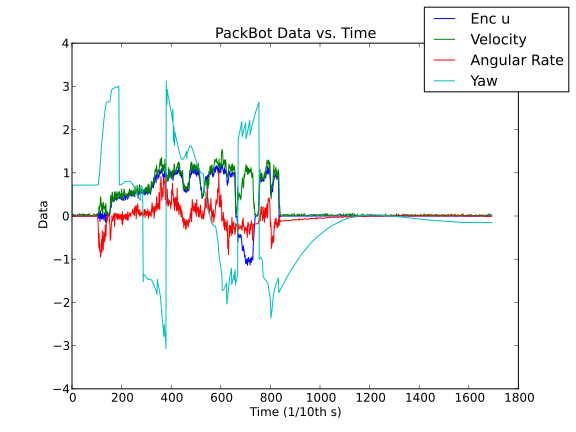
\includegraphics[width=.8\textwidth]{images/pbDataReverseHeading}
	\caption{Heading and Velocity Reversed}
	\label{fig:pbDataReverseHeading}
\end{figure}

*** Figure \ref{fig:pbDataReverseHeading} used encoders and GPS for linear velocity measurements, Microstrain and GPS for heading measurements and Microstrain for yaw rate measurement. The Kalman filter output for heading and the GPS velocity measurements can be seen to flip $180^\circ$ when the robot starts to drive in reverse but the encoders accurately measure the direction of the velocity vector. During the time that the robot is driving in reverse the yaw rate stays slightly negative so the yaw value should be decreasing slightly. The robot drives in reverse from about $65 s - 76s$ as noted in the image. ***

\subsection{Additional Sensors}
\label{sec:kfAdditionalSensors}
*** Talk about adding the compass and using encoder data. ***

\section{Identifty IMU Parameters}
\label{sec:identifyimuparams}
*** Looking at \cite{ChungOjeda01}. Would need access to a rotary table to perform tests. Also look at \cite{ParkinsonHeadingEstimation01} for better estimation of heading. ***

\chapter{Controls}
\label{ch:controls}
Control systems are responsible for computing the commands necessary for actuators to cause the trajectory of a system to go from its current state to a desired state, or for answering the question "How do I get there?". There are many different methods that can be used to determine the output commands. One of the more popular and widely implemented control systems is the PID (Proportional, Integral, Differential) controller. Model based controllers utilize knowledge of the physics of the system to compute appropriate output commands. The robots in these experiments originally used PID controllers for heading control and were later tested with a model based contoller that takes advantage of Lyapunov stability theory. Both types of controllers described in this Chapter take in state estimates from the Kalman filter from Chapter \ref{ch:estimation} and output linear and angular velocity commands to the robots.

\section{PID}
\label{sec:pid}
PID controllers use the current state estimate to determine the errors between the desired state and the current state. The goal of the PID controller is to drive those errors to zero based on a number of criteria including rise time, settling time, steady state error and overshoot as shown in Figure \ref{fig:pid} where the green line is the ideal output while the blue and purple lines are typical results. The orange line shows what happens when a system becomes unstable. Point $m$ represents the desired state, $m-n$ represents steady state error, point $a$ is the rise time for the blue line and point $b$ is the settling time for the blue line.

\begin{figure}[ht!]
	\centering
	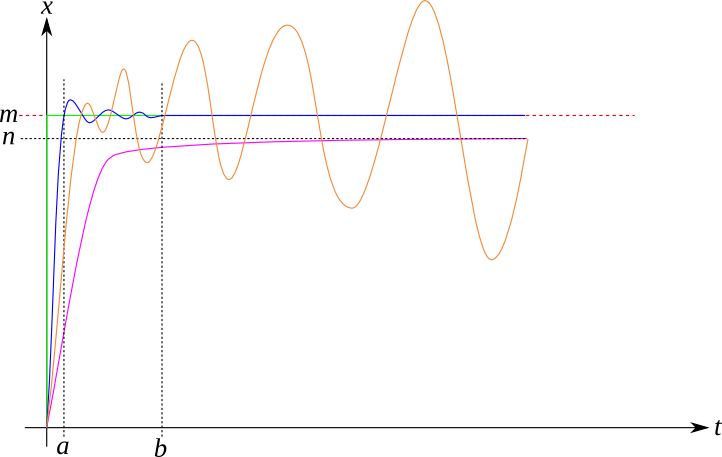
\includegraphics[width=.85\textwidth]{images/pid}
	\caption{PID Controller Responses} 
	\label{fig:pid}
\end{figure}

There are separate PID controllers used for robot distance ($e$) and heading errors ($\psi$). The process used to compute an output command using a PID controller uses three separate errors and a gain for each of the distance and heading errors. Looking at the PID controller for heading the errors are
\begin{align*}
%\label{eq:piderrors}
\begin{split}
E_P &= \psi_{\text{ref}_k} - \psi_k \\
E_I &= \sum_{i=0}^{k}E_{P_i}*\Delta_T \\
E_D &= \frac{\psi_k - \psi_{k-1}}{\Delta_T}
\end{split}
\end{align*}
where $\psi_{\text{ref}_k}$ is the desired heading at the current time, $\psi_k$ is the current heading estimate, $\psi_{k-1}$ is the previous heading estimate and $\Delta_T$ is the time elapsed since the last PID control calculation was performed. The contribution of each error is then weighted by a gain to obtain the final output command, $u$, such that
\begin{align*}
%\label{eq:pidcommand}
u = K_P*E_P + K_I*E_I + K_D*E_D
\end{align*}
where $K_P$ is the proportional gain, $K_I$ is the integral gain and $K_D$ is the differential gain.

The only parameters available to tune PID controllers for performance are the gains. There are some rules of thumb for tuning gains properly as described in \cite{ZeiglerNichols42} that can work as a good starting point, along with a basic knowledge of what the effects are of modifying the different gains as summarized in Table \ref{tab:PIDGainEffects}. The difficulty in using PID controllers for the small robots used in these experiments is that the gains must be tuned for specific operating scenarios so that a set of gains that work well at full speed on asphalt do not work at all when the robot is driving in soft sand at any velocity. PID controllers work best when they only have to reject a small range of disturbances, however the small robots are often required to operate in environments with a large range of disturbances.

When the characteristics of a robot are changed the PID gains must also be modified to reflect those changes. These characteristics include mass, center of mass, particular treads, motors and payloads as these all affect the dynamics of the system. Gain scheduling is the process of tuning a system to use a different set of gains based on the operating environment or characteristics of the robot and is very time consuming. This motivates the search for a better control system for these small robots.

Table \ref{tab:PIDGainEffects} shows how increasing the different gain values affects the performance of the controller output in terms of rise time, overshoot, settling time and steady state error. It can be seen that a large amount of coupling exists between the gains and attempting to fix one aspect of the controller output can have unintended consequences that cause other aspects of controller output to perform suboptimally. This is in contrast to the gains that arise for model based controllers as seen in Chapter \ref{sec:lyapunovTrajectoryConvergence}.

\begin{table}[ht!]
\caption{Effects on Controller Output of Modifying PID Gains}
\small
\centering
\begin{tabular}{@{}llllr@{}} \toprule
Parameter    & Rise Time      & Overshoot & Settling Time & Steady State Error \\ \midrule
$K_p$        & Decrease       & Increase  & Small Change  & Decrease \\
$K_i$        & Decrease       & Increase  & Increase      & Eliminate \\
$K_d$        & Small Decrease & Decrease  & Decrease      & None \\ \bottomrule
\end{tabular}
\label{tab:PIDGainEffects}
\end{table}

\subsection{PID Implementation}
The PID controller used by SSCPAC was only for angular rate output while the linear velocity output was set to a maximum allowable velocity and then a simple ramp function was used to slow the robot down as it approached a waypoint. In conjunction with the PID controller a simple local path planner was developed following work in \cite{Hogg02} in which a carrot is placed a reasonable distance in front of the robot on the path from the previous to the current waypoint and the carrot position was used to correct the heading. This causes the PID controller to move the robot onto that path faster than it would if the heading error were only based on the angle to the waypoint when the waypoint is a large distance from the robots current position. The carrot could also be extended along the path so that the robot would not stop at each intermediate waypoint but would instead cut the corner on the way to the next waypoint. One of the difficulties in using the PID controller, and a motivation for finding a different control scheme, is that as the maximum allowable linear velocity was set to larger values the performance of the controller would work poorly when the waypoints were spaced close together as is the case when obstacles are present. The converse is also true. As mentioned previously gain scheduling is a time intensive task but it is possible that it would have provided a working solution.

\section{Model Based Controller}
\label{sec:lyapunov}
The motivation to find a replacement for the PID controller was caused by one major shortcoming. When the PID gains were set to work well when the robot was running at full speed the robot did not work well when slowing down, as is typically the case when obstacles are encountered. Tuning the gains to work well at slow speeds caused the robot to drive poorly at fast speeds. As will be shown in Chapter \ref{ch:results} the model based controller works well at varying speeds. There are also cases where the PID controller becomes unstable and cannot converge to a goal position. The model based controller does not suffer from this deficiency.

An alternative control method to using classical PID controllers is to use model based controllers based on Lyapunov stability theory. An intuitive way to conceptualize controllers based on this stabilty theory is by thinking of them as decreasing the overall energy of a system, even when the variables involved in the control Lyapunov functions do not represent energy \cite{Khalil02}.

The theorem for Lyapunov stability states that for an equilibrium point $x=0$ and a domain $D\subset\mathbb{R}^n$ that contains $x=0$ and for which there is a function $V:D\to\mathbb{R}$ that is continuously differentiable and has the following properties 
\begin{align}
\label{eq:lyapunovTheorem}
\begin{split}
V(0) &= 0 \\
V(x) &> 0 \in D-\{0\} \\
\dot{V}(x) &\leq 0 \in D-\{0\}
\end{split}
\end{align}
then the equilibrium point $x=0$ is stable. Additionally, if
\begin{align}
\label{eq:lyapunovAsymptoticStability}
\dot{V}(x) < 0 \in D - \{0\}
\end{align}
then $x=0$ is asymptotically stable.

It is not always possible to find such a control Lyapunov function $V$ but when one is found then this theorem holds and the "energy" of the system will always be positive and decreasing. The "energy" can consist of any variables that make $V(0) = 0$ and $V(x) > 0$ and consist of a combination of the errors that are to be minimized in a system. In that case the errors are always decreasing since $\dot{V}(x) < 0$ and the system will reach the desired state.

Two different modes of the model based controller were developed and tested during these experiments. The difference between the two modes is the behavior of the robot as it approaches intermediate waypoints while navigating to its final destination. The first mode is considered to be useful for a parking behavior where the robot stops at each waypoint including the intermediate waypoints. The second mode is a slightly modified version of the parking behavior where the distance error is extended beyond each intermediate waypoint so that the robot will drive through the waypoints without stopping (although the robot often does slow down some) until it reaches its final destination. This second mode will be referred to as the driving mode. During the following development of the control law the parking mode will be described fully and then extensions will build directly on top of the parking mode to describe the driving mode in Chapter \ref{sec:drivingMode}.

\subsection{Unicycle-like Robot Kinematics}
\label{sec:unicycleKinematics}
Several groups have implemented model based controllers rooted in Lyapunov stability theory in simulation including \cite{MicaelliLyapunov93}, \cite{Aicardi94}, \cite{Aicardi_UnicycleLyapunov95}, \cite{Rusu05RobotuxLyapunov}, \cite{Gulati08} but only recently have these results been applied to actual robots \cite{KimLyapunov05}, \cite{Lapierre06}, \cite{Lapierre07}, \cite{NuchterLyapunov07}. All of these groups describe a method for constructing a control Lyapunov function based on the kinematics of a differential drive robot, similar in nature to the small robots considered in these experiments and typically referred to as unicycle-like robots in the literature.

\begin{figure}[ht!]
	\centering
	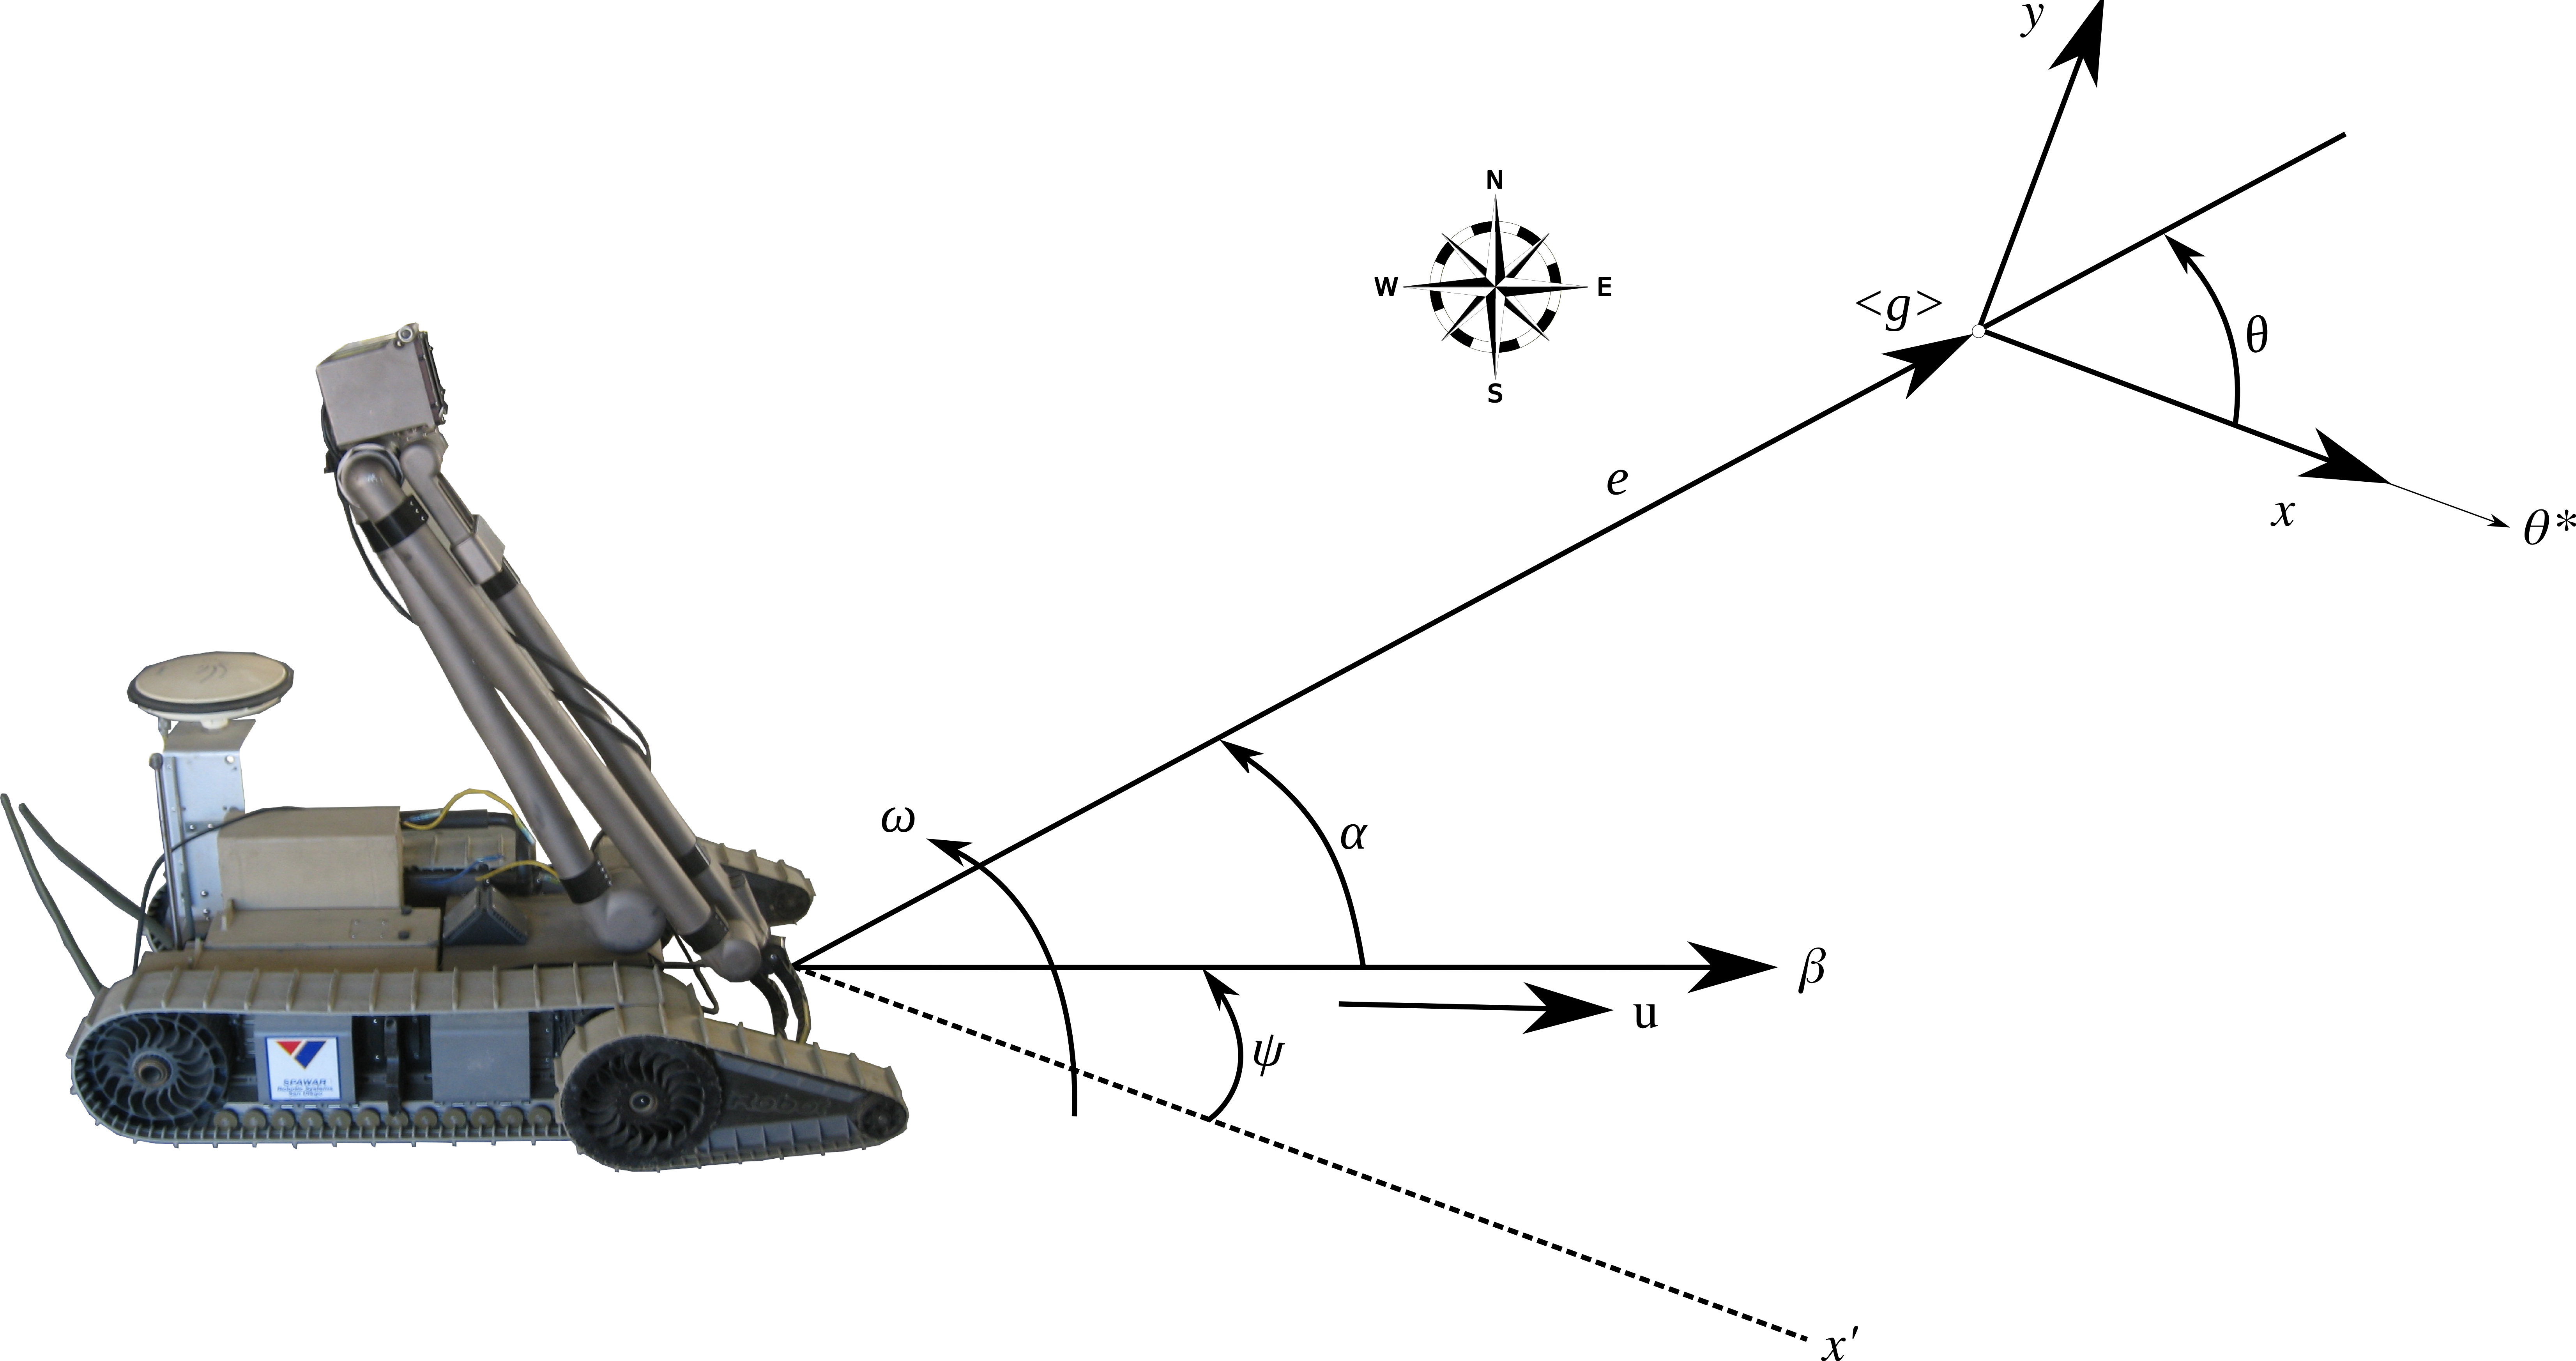
\includegraphics[width=.95\textwidth]{images/packbotlyapunov}
	\caption{Packbot Coordinate System for Model Based Controller}
	\label{fig:pblyapunov}
\end{figure}

Figure \ref{fig:pblyapunov} will be used as the basis for the equations that follow and will be explained in further detail here. Since life is never easy this controller has been developed with the global $x$-axis pointing East, the local $x$-axis pointing to the right of the robot while the global $y$-axis is North and the local $y$-axis is pointing forward of the robot. Since the Kalman filter has the local $x$-axis forward and the local $y$-axis pointing left the yaw state has to be transformed into the new coordinate system.

Given a robot at some arbitrary initial position we want it to move to a goal position with a specific heading where the goal position is the origin of the $<g>$ coordinate system and the desired heading is along the $x$-axis of the $<g>$ coordinate system labeled $\theta^\star$. The states that define the robot's current position, heading, and linear and angular velocities are calculated using the Kalman filter of Chapter \ref{sec:extendedkf} whereas the goal position and heading are given as inputs to the robot. Note that the linear velocity is given by $u$ and the angular velocity by $\omega$.

The control system attempts to force three separate errors to zero:
\begin{itemize}
\item $e$, the magnitude of the translation error vector as measured between the current position and goal position,
\item $\theta$, the angle between the desired heading and the translational error vector $e$,
\item $\alpha$, the angle between the current heading and the translational error vector $e$.
\end{itemize}

The reason that those three particular errors were selected is driven by the fact that the robots are nonholonomic (they are only able to move forwards or backwards along the direction of their current heading and cannot move sideways). For holonomic robots a reasonable controller that gets the robot to a desired position with a desired heading would simply move at an angle towards the goal position and along the way correct its heading. Since that is not possible for the robots here some tradeoffs are required and those come in the form of the two angle errors, $\theta$ and $\alpha$. One way that a controller for nonholonomic vehicles could work is to rotate until the robot is pointed towards the goal position, then move in a straight line to the goal position and finally rotate in place again to the desired heading. However, that is boring and not very efficient as it would mean that the robot would have to stop at each waypoint along a route so that it could correct its heading to point to the next waypoint. The approach taken with the model based controller described here is to let the robot have the ability to align itself with the goal heading by zeroing out $\theta$ and $\alpha$ before it arrives at the goal position. This approach will allow the robot to maintain speed when it arrives at intermediate waypoints along the route.

Additional variables used to calculate the errors and shown in Figure \ref{fig:pblyapunov} include:
\begin{itemize}
\item $\theta^\star$, the target heading in the global coordinate system which is aligned with the $x$-axis of $<g>$,
\item $\theta_e$, the angle of the error vector in the global coordinate system,
\item $\psi$, the current heading of the robot in the global coordinate system,
\item $\phi$, the difference between the target heading and the current heading in the global coordinate system.
\end{itemize}

A kinematic model of the robot is used to predict how the robot moves without considering the effects of the mass of the robot or outside forces (such as friction between the robot tracks and the ground) acting on the robot with
\begin{align}
\label{eq:lyapunovkinematics1}
\begin{split}
\dot{x} &= u\cos\phi \\
\dot{y} &= u\sin\phi \\
\dot{\phi} &= \omega.
\end{split}
\end{align}
The expressions in (\ref{eq:lyapunovkinematics1}) are then converted to a polar coordinate representation via a coordinate transformation and give expressions for the errors that the control system is attempting to drive to zero such that
\begin{align}
\label{eq:lyapunovPolar}
\begin{split}
e &= \sqrt{x^2+y^2} \\
\theta &= \atanh(y,x) \\
\alpha &= \theta - \phi.
\end{split}
\end{align}
Combining (\ref{eq:lyapunovPolar}) with (\ref{eq:lyapunovkinematics1}) results in
\begin{align*}
%\label{eq:lyapunovkinematics3}
\begin{split}
\dot{e} &= -u*\cos(\theta-\phi) \\
\dot{\theta} &= u\frac{\sin\alpha}{e} \\
\dot{\phi} &= \omega.
\end{split}
\end{align*}
Finally, replacing $\alpha$ with $\theta-\phi$ results in a kinematic model of
\begin{align}
\label{eq:lyapunovkinematics}
\begin{split}
\dot{e} &= -u\cos\alpha \\
\dot{\alpha} &= -\omega + u\frac{\sin\alpha}{e} \\
\dot{\theta} &= u\frac{\sin\alpha}{e}.
\end{split}
\end{align}

\subsection{Control Lyapunov Function}
\label{sec:controllyapunov}
The control Lyapunov function is selected to be positive, contain all three error states and separate the distance error from the angle errors and is given by
\begin{align}
\label{eq:lyapunovfunction}
V = V_1 + V_2 = \frac{1}{2}\lambda e^2 + \frac{1}{2}\left(\alpha^2+h\theta^2\right)
\end{align}
where $\lambda$ and $h$ are positive constants that can be used to tune the controller output (see Chapter \ref{sec:lyapunovTrajectoryConvergence}). Using the kinematics equations in (\ref{eq:lyapunovkinematics}) the derivative of each term of the candidate control Lyapunov function can be found as
\begin{align}
\label{eq:Vderivatives}
\begin{split}
\dot{V}_1 &= \lambda e\dot{e} = \lambda e (-u\cos\alpha) = -\lambda eu\cos\alpha \\
\dot{V}_2 &= \alpha\dot{\alpha}+h\theta\dot{\theta} \\
&= -\alpha\omega + \alpha u\frac{\sin\alpha}{e} + h\theta u\frac{\sin\alpha}{e} \\
&= \alpha\left(-\omega + u\frac{\sin\alpha}{e} + h\theta u\frac{1}{\alpha}\frac{\sin\alpha}{e}\right) \\
&= \alpha\left(-\omega + u\frac{\sin\alpha}{\alpha}\frac{(\alpha+h\theta)}{e}\right)
\end{split}
\end{align}
and from (\ref{eq:Vderivatives}) the total derivative is found as
\begin{align}
\label{eq:lyapunovfunctionderivative}
\begin{split}
\dot{V} &= \dot{V}_1 + \dot{V}_2 = -\lambda e u\cos\alpha + \alpha\left(-\omega+u\frac{\sin\alpha}{\alpha}\frac{(\alpha+h\theta)}{e}\right).
\end{split}
\end{align}

Now it needs to be shown that $\dot{V}\leq0$ which can be done by showing that $\dot{V}_1\leq0$ and $\dot{V}_2\leq0$. This is true for $\dot{V}_1$ if $u$ takes the form
\begin{align}
\label{eq:lyapunovu}
u = \gamma e\cos\alpha
\end{align}
where $\gamma$ is a positive constant different from $\lambda$. Substituting this value of $u$ into (\ref{eq:Vderivatives}) results in
\begin{align}
\label{eq:V1dotfinal}
\dot{V}_1 = -\lambda eu\cos\alpha = -\lambda\gamma e^2\cos^2\alpha \leq 0.
\end{align}
Since $V_1\geq0$ and $\dot{V}_1\leq0$ we have that $V_1$ converges asymptotically to a positive defined limit.

Replacing $u$ in the expression for $\dot{V}_2$ in (\ref{eq:Vderivatives}) results in
\begin{align}
\label{eq:V2dotreplaceu}
\begin{split}
\dot{V}_2 &= \alpha\left(-\omega+u\frac{\sin\alpha}{\alpha}\frac{(\alpha+h\theta)}{e}\right) \\
&= \alpha\left(-\omega+\gamma e\frac{\cos\alpha\sin\alpha}{\alpha}\frac{(\alpha+h\theta)}{e}\right) \\
&= \alpha\left(-\omega+\gamma(\alpha+h\theta)\frac{\cos\alpha\sin\alpha}{\alpha}\right).
\end{split}
\end{align}

Similarly, $\dot{V}_2$ is negative definite if $\omega$ takes the form
\begin{align}
\label{eq:lyapunovomega}
\begin{split}
\omega &= k\alpha + \gamma\frac{\cos\alpha\sin\alpha}{\alpha}\left(\alpha+h\theta\right)
\end{split}
\end{align}
where $k$ is a positive constant. Substituting this value of $\omega$ into (\ref{eq:V2dotreplaceu}) gives
\begin{align}
\label{eq:V2dotfinal}
\begin{split}
\dot{V}_2 &= \alpha\left(-k\alpha-\gamma\frac{\cos\alpha\sin\alpha}{\alpha}(\alpha+h\theta) + \gamma\frac{\cos\alpha\sin\alpha}{\alpha}(\alpha+h\theta)\right) \\
&= -k\alpha^2 \leq 0
\end{split}
\end{align}
and $V_2$ converges asymptotically to a positive defined limit.

Substituting $\dot{V}_1$ from (\ref{eq:V1dotfinal}) and $\dot{V}_2$ from (\ref{eq:V2dotfinal}) into the expression for $\dot{V}$ (\ref{eq:lyapunovfunctionderivative}) yields
\begin{align*}
%\label{eq:Vdotfinal}
\dot{V} = \dot{V}_1 + \dot{V}_2 = -\lambda\gamma e^2\cos^2\alpha - k\alpha^2 \leq 0.
\end{align*}
This expression is equal to zero if and only if $\alpha=0$ \textit{and} $e=0$, which only occurs when the robot has reached its goal pose. Additionally, it can be shown that $\theta=0$ when $\dot{V}=0$ by invoking Barbalat's lemma \cite{Aicardi_UnicycleLyapunov95}. Therefore, at any point along the robots trajectory other than the goal position and heading this function is negative definite and satisfies the properties for asymptotic stability given by (\ref{eq:lyapunovTheorem}) and (\ref{eq:lyapunovAsymptoticStability}).

Using the expressions for $u$ in (\ref{eq:lyapunovu}) and $\omega$ in (\ref{eq:lyapunovomega}) and substituting those values back into the kinematic model from (\ref{eq:lyapunovkinematics}) gives
\begin{align}
\label{eq:lyapunovfinalkinematics}
\begin{split}
\dot{e} &= -u\cos\alpha = -\gamma e\cos^2\alpha \\
\dot{\alpha} &= -\omega + u\frac{\sin\alpha}{e} \\
&= -(k\alpha+\gamma\frac{\cos\alpha\sin\alpha}{\alpha}(\alpha+h\theta))+\gamma e\cos\alpha\frac{\sin\alpha}{e} \\
&= -k\alpha-\gamma\cos\alpha\sin\alpha+\gamma\cos\alpha\sin\alpha-\gamma h\theta\frac{\cos\alpha\sin\alpha}{\alpha} \\
&= -\left(k\alpha + \gamma h\theta\frac{\cos\alpha\sin\alpha}{\alpha}\right) \\
\dot{\theta} &= u\frac{\sin\alpha}{e} = \gamma e\cos\alpha\frac{\sin\alpha}{e} = \gamma\cos\alpha\sin\alpha
\end{split}
\end{align}

Combining (\ref{eq:lyapunovu}) and (\ref{eq:lyapunovomega}) gives the following control law to replace the PID controller from Chapter \ref{sec:pid}:
\begin{align}
\label{eq:lyapunovControlLaw}
\begin{split}
u &= \gamma e\cos\alpha \\
\omega &= k\alpha + \gamma\frac{\cos\alpha\sin\alpha}{\alpha}\left(\alpha+h\theta\right)
\end{split}
\end{align}

\subsection{Calculating Control Law Variables}
\label{sec:lyapunovVariables}
The method used to calculate the variables needed for the control law in (\ref{eq:lyapunovControlLaw}) based on Figure \ref{fig:pblyapunov} is:
\begin{enumerate}
\item $dx_e$ is the horizontal component of the error vector $e$ as seen in Figure \ref{fig:pblyapunov}.
\item $dy_e$ is the vertical component of the error vector $e$ as seen in Figure \ref{fig:pblyapunov}.
\item Use $e = \sqrt{dx_e^2 + dy_e^2}$ to get the distance to the waypoint on the current path segment.
\item $\psi$ is the current heading of the robot in the world coordinate frame and is calculated in the Kalman filter based on the results from Chapter \ref{ch:estimation}. Note that this has to be rotated so that it works in the current coordinate system.
\item $\theta_e$ is the angle of the error vector $e$ and is found as $\theta_e = \text{atan2}(dy_e,dx_e)$.
\item $\theta^\star$ is the desired heading in the global coordinate system and there are multiple ways that it \textit{could} be set. Suppose that the robot is between waypoint $1$ and waypoint $2$ on a route and that waypoint $3$ exists and the waypoints have coordinates given by $(x_1,y_1)$, $(x_2,y_2)$ and $(x_3,y_3)$. Then,
\begin{itemize}
\item $\theta^\star=0$ sets the desired heading as East and $\theta^\star=\frac{\pi}{2}$ sets it as North.
\item $\theta^\star=\psi$ would make the desired heading be the same as whatever the current heading happens to be.
\item $\theta^\star$ can be sent in as an additional parameter of a waypoint, say from MOCU via JAUS.
\item $\theta^\star$ can be the angle from the previous waypoint to the current waypoint. This is found by using $dx_{\theta^\star}=x_2-x_1$, $dy_{\theta^\star}=y_2-y_1$ and $\theta^\star=\text{atan2}(dy_{\theta^\star},dx_{\theta^\star})$.
\item $\theta^\star$ can be the angle from the current waypoint to the next waypoint. This is found by using $dx_{\theta^\star}=x_3-x_2$, $dy_{\theta^\star}=y_3-y_2$ and $\theta^\star=\text{atan2}(dy_{\theta^\star},dx_{\theta^\star})$.
\end{itemize}
\item $\phi=\theta^\star-\psi$.
\item $\theta=\theta^\star - \theta_e$.
\item $\alpha = \theta - \phi$.
\end{enumerate}

\subsection{Model Based Driving Mode}
\label{sec:drivingMode}
The parking mode described above can be extended such that the control law will cause the robot to drive through intermediate waypoints on a route rather than stop at each waypoint. The basic idea is that the target position as given in the goal frame $<g>$ of Figure \ref{fig:pblyapunov} is moved such that the distance error $e$ is increased. Since the linear velocity output of the controller is a function of $e$ (c.f. (\ref{eq:lyapunovControlLaw})) that output will increase causing the robot to drive faster through the intermediate waypoints. As described in \cite{Aicardi_UnicycleLyapunov95} an effective means of moving the goal frame is to control its rate of motion, $\dot{s}$, via the function
\begin{align}
\label{eq:moveTargetFrame}
\dot{s} =
\begin{cases}
0, & V = \lambda e^2 + (\alpha^2+h\theta^2) > \epsilon \\
f(e,\alpha,\theta), & V = \lambda e^2 + (\alpha^2+h\theta^2) \leq \epsilon
\end{cases}
\end{align}
where $0<\epsilon<\frac{\pi^2}{4}$. The function $V$ describes an ellipsoid such that if any of the errors are larger than the threshold given by $\epsilon$ then the goal frame will not be moved and the parking behavior will be used. When the robot is aligned with both the waypoint and the desired heading, causing $(\alpha,\theta)=(0,0)$, then a reasonable course of action is to maintain the maximum allowable linear velocity and it is for this reason that the design variable $\lambda$ is typically chosen to be very small to limit the amount of influence that the distance error has on the motion of the goal frame. The implemented function to move the goal frame according to (\ref{eq:moveTargetFrame}) was selected to be
\begin{align}
\label{eq:moveTargetFrameFunction}
f(e,\alpha,\theta) = u_{\text{max}} * \text{max}\left(0, 1 - \frac{V}{\epsilon}\right).
\end{align}
It can be seen from (\ref{eq:moveTargetFrame}) and (\ref{eq:moveTargetFrameFunction}) that by setting $\epsilon$ to a small value makes it more difficult for the system to enter the ellipsoidal domain where $V\leq\epsilon$ and also decreases the amount of motion for the goal frame. Note that setting $\epsilon=0$ results in the parking mode since $\dot{s}=0$ and the goal frame never moves.

The resulting behavior of the robot has a very natural appearance as this is how humans typically drive. When the road ahead is straight and we want to continue driving straight we keep our eyes focused further down the road and maintain speed. However, when the road ahead is twisty or we want to make a turn we slow down and focus our eyes closer to our current position.

\subsection{Practical Considerations for Selecting Gains}
\label{sec:lyapunovTrajectoryConvergence}
The gains $h$, $k$ and $\gamma$ in the control law (\ref{eq:lyapunovControlLaw}) determine the resulting trajectory that the robot will use when driving from its current position to the goal point and heading. The first thing to notice is that the linear velocity is at a maximum when the angle error $\alpha=0$ since that leads to $\cos(\alpha)=1$ and $u_{\text{max}}=e\gamma$. As discussed in Chapter \ref{sec:lyapunovVariables} a carrot can be set by the path planner to limit the maximum error distance $e$ so that $e$ is bounded. When that is the case the maximum linear velocity is proportional to the gain $\gamma$. For example, if the carrot has a maximum lookahead distance of $10m$ and $\gamma=0.2$ then $u_{\text{max}}=10*0.2=2\tfrac{m}{s}$ which is a reasonable limit for a Packbot.

There are many ways to select what values the gains $h$ and $k$ should take, especially once $\gamma$ is set, and some of the properties of the kinematics equations (\ref{eq:lyapunovfinalkinematics}) as the angle errors $(\alpha, \theta)$ approach $(0, 0)$ are helpful in making those selections as the system involving the errors to be minimized is approximately linear. The key to this linearization is to notice that when $\alpha$ is near zero several terms in (\ref{eq:lyapunovfinalkinematics}) cancel out since $\alpha\to0\Rightarrow \alpha=\cos(\alpha)*\sin(\alpha)=\sin(\alpha)$ as seen in Figure \ref{fig:plotSinCos}. When that is the case the following linear approximation holds:
\begin{align}
\label{eq:lyapunovLinearSystem}
\begin{split}
\left[\begin{array}{c} \dot{\alpha} \\ \dot{\theta} \end{array}\right]
&= \underbrace{\left[\begin{array}{c c} -k & -h\gamma \\ \gamma & 0 \end{array}\right]}_{A}
\left[\begin{array}{c} \alpha \\ \theta \end{array}\right] \\
\dot{e} &= -\gamma e
\end{split}
\end{align}
with linear output equations
\begin{align}
\label{eq:lyapunovLinearOutput}
\begin{split}
u &= \gamma e \\
\omega &= (k+\gamma)\alpha + h\gamma\theta.
\end{split}
\end{align}

\begin{figure}[ht!]
	\centering
	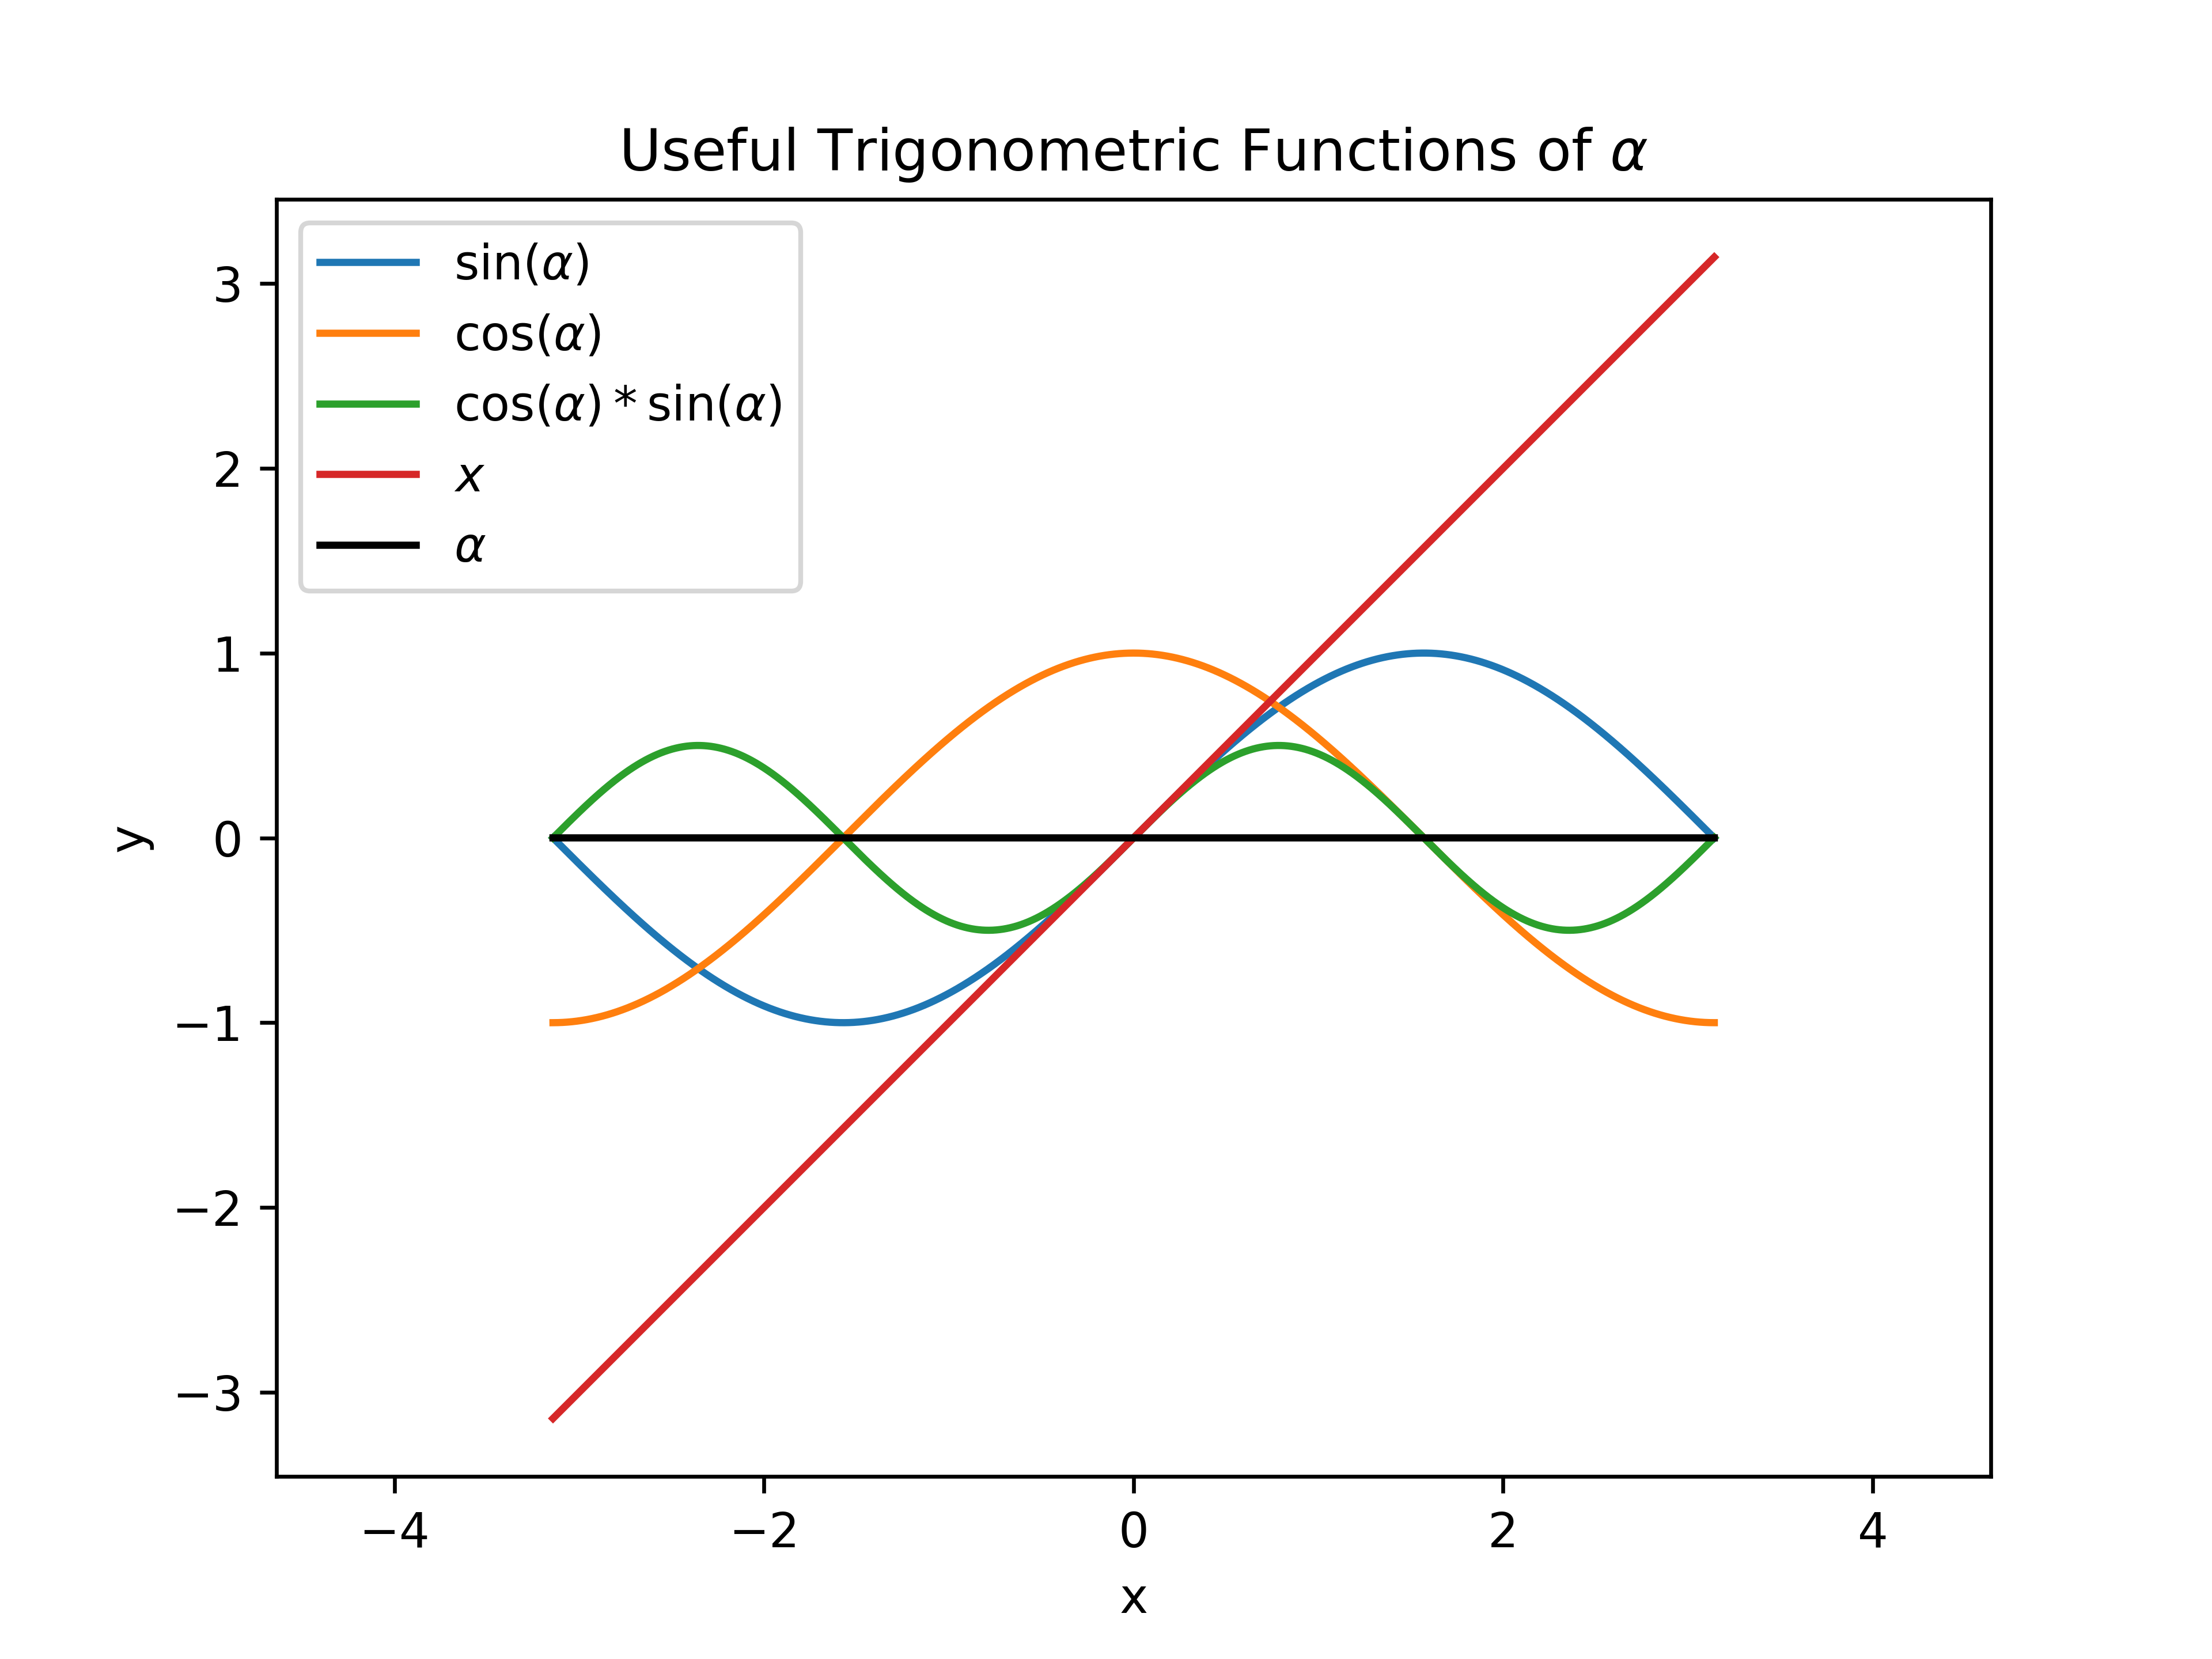
\includegraphics[width=.75\textwidth]{images/plotSinCos}
	\caption{Useful Trigonometric Functions of $\alpha$}
	\label{fig:plotSinCos}
\end{figure}

This shows that, in the neighborhood of $(\alpha, \theta)=(0, 0)$, the distance error $e$ converges linearly at a rate of $-\gamma$ while the angle errors converge at a rate of $-\sigma$ where $-\sigma$ is the real part of the dominant pole of the linear system $A$ in (\ref{eq:lyapunovLinearSystem}) which can be found from the eigenvalues of $A$. The reason that the errors converge at those rates is that, for the distance error, $e=\text{exp}(-\gamma t)$ is a solution to the equation $\dot{e}=-\gamma e$ since 
\begin{align*}
\tfrac{d}{dt}e=\tfrac{d}{dt}\text{exp}(-\gamma t) = -\gamma \text{exp}(-\gamma t)=-\gamma e.
\end{align*}
Similarly, the behavior of the angle errors is related to the matrix $A$ and nonsingular matrices can be factored into the form $A=S\Lambda S^{-1}$ where $S$ contains the eigenvectors of $A$ and $\Lambda$ is a diagonal matrix containing the eigenvalues of $A$. The solution to the differential equation is
\begin{align*}
\left[\begin{array}{c} \dot{\alpha} \\ \dot{\theta} \end{array}\right] = \text{exp}(At)=\text{exp}(S\Lambda S^{-1}t)=S\text{exp}(\Lambda t)S^{-1}
\end{align*}
and $\dot{\alpha}$ has the solution $\alpha=\text{exp}(\lambda_\alpha t)$ and $\dot{\theta}$ has the solution $\theta=\text{exp}(\lambda_\theta t)$.

In parking mode three reasonable design considerations in selecting the gains are:
\begin{itemize}
\item limit the maximum linear velocity,
\item find critically damped gains,
\item have angle errors converge before distance error.
\end{itemize}
Limiting the maximum linear velocity has been discussed already and involves the selection of $\gamma$. The damping of the system $A$ is determined by
\begin{align*}
\zeta = \frac{\lambda_\alpha(A)}{\lambda_\theta(A)}
\end{align*}
and the gains are critically damped when $\zeta = 1 \Rightarrow \lambda_\alpha(A)=\lambda_\theta(A)=\lambda$ so that both angle errors $\alpha$ and $\theta$ are converging to zero at the same rate. When the system is critically damped the angle errors will converge before the distance error if $\sigma>\gamma$ since that means the rate of convergence for the angle errors is greater than the rate of convergence for the distance error. In the case where the $A$ matrix is overdamped $\zeta > 1 \Rightarrow \lambda_\alpha(A) > \lambda_\theta(A)$ then $\alpha$ will converge to zero before $\theta$ and conversely when $A$ is underdamped $\zeta < 1$ and $\theta$ converges before $\alpha$.

By selecting the gains to satisfy the design considerations above the robot will align itself with the goal heading before arriving at the goal point and will smoothly decrease its linear velocity as it approaches the goal point. One alternative occurs when the distance error converges before the angle errors, $\gamma>\sigma$, and the robot will get to the goal point and then finish aligning with the goal heading which has several problems: (i) the robot does not look as intelligent since the trajectory does not appear to be as "natural" as the way a human would drive and (ii) rotating in place is typically a much more difficult maneuver for tracked robots to perform and increases the fatigue on the treads compared to turning while driving forward.

To deterministically discover gains that will satisfy the properties discussed two conditions must be met:
\begin{itemize}
\item $\zeta = 1$
\item $\sigma > \gamma$
\end{itemize}
For $\zeta=1$ it is necessary to first determine the eigenvalues of $A$.
\begin{align*}
&(A-\lambda I) = \left[\begin{array}{c c} -k-\lambda & -h\gamma \\ \gamma & -\lambda\end{array}\right] = 0 \\
\Rightarrow &(-k-\lambda)(-\lambda)+h\gamma^2 = 0 \\
\Rightarrow &\lambda^2 + k\lambda + h\gamma^2 = 0 \\
\Rightarrow &\lambda = \frac{-k\pm\sqrt{k^2-4h\gamma^2}}{2}
\end{align*}
For $\lambda_\alpha(A)=\lambda_\theta(A)$ the term inside the square root must be equal to zero resulting in
\begin{align*}
&k^2 - 4h\gamma^2 = 0 \\
\Rightarrow &k = \sqrt{4h\gamma^2} = 2\gamma\sqrt{h}
\end{align*}
To find $\sigma>\gamma$ constrained by $k=2\gamma\sqrt{h}$ it is necessary to have
\begin{align*}
\sigma &= -\lambda = \tfrac{k}{2} > \gamma \\
\Rightarrow k &> 2\gamma
\end{align*}
The two equations can be combined to find $h$ such that
\begin{align*}
k &= 2\gamma\sqrt{h} > 2\gamma \\
\Rightarrow h &> 1
\end{align*}

Using this method any two gains can be selected and the third gain can be found which satisfies the above properties. For example, setting $\gamma=0.2$ to limit the maximum linear velocity and $h=1.1$ to keep it small but greater than one leads to $k=2\gamma\sqrt{h}=0.42$. From this it can be seen that $\lambda_\alpha(A) = \lambda_\theta(A) = 0.21 \Rightarrow \zeta = 1$ so the system $A$ is critically damped and $\sigma = 0.21>0.2=\gamma$ so that the angle errors will converge before the distance error.

When using (\ref{eq:moveTargetFrame}) to move the goal frame and put the robot into driving mode it can be more desirable to generate trajectories such that the robot stays on a straight line path to the next waypoint so that the angle errors are decreased and drives faster. One way to have the robot drive towards the waypoint is to set the gains such that the distance error converges before the angle errors and have $\alpha$ converge before $\theta$. An example of the gains that produce these effects is $\gamma=0.25$, $h=0.33$ and $k=0.30$. Another way to cause the robot to drive on the line segment connecting the previous and current waypoints is to have the target heading be set as the angle from the previous waypoint to the current waypoint.

The model based controller developed in this Chapter along with the analysis of selecting appropriate gains replaces the original PID controller when answering the question "How do I get there?".

\chapter{Results}
\label{ch:results}
The Kalman filter and controls algorithms discussed in this thesis were implemented in software on a PackBot and run in an open field with an uneven surface consisting of dirt, gravel and asphalt. This testing area is difficult for the robots to navigate because pitch, roll and elevation change and the loose dirt and gravel cause the tracks to slip leading to erroneous encoder data.

\section{Kalman Filter Results}
\label{sec:kfResults}
Model based with original noise models.

\begin{figure}[ht!]
	\centering
	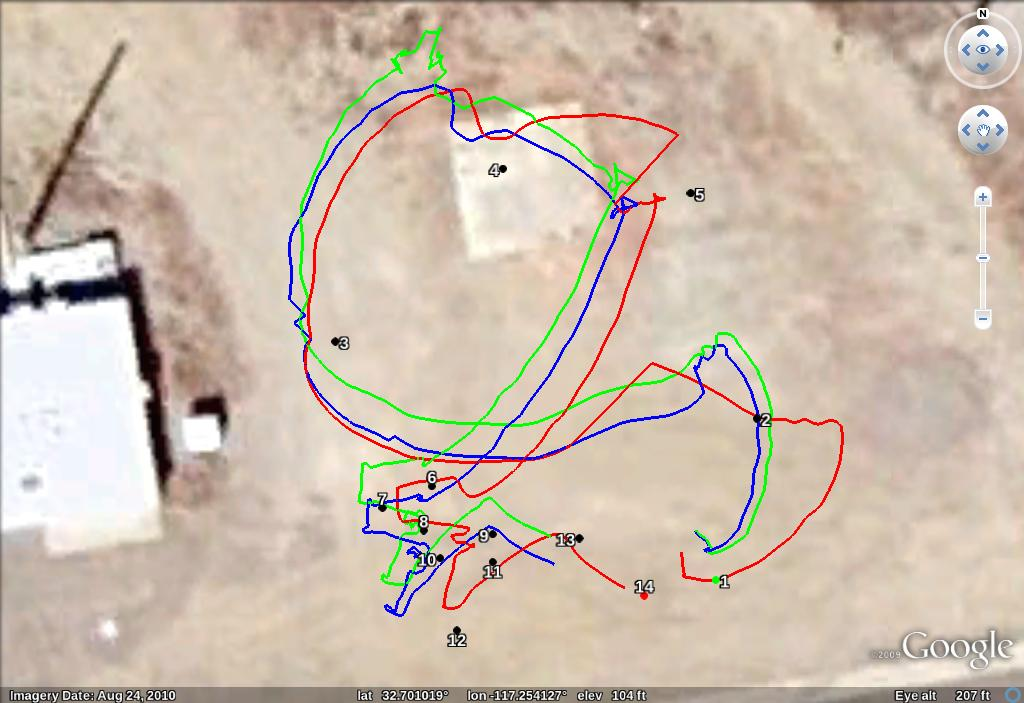
\includegraphics[width=.5\textwidth]{images/GE/20101203_1551_kf_lyapOrigQR}
	\caption{Model Based Controller with Original Noise Models}
	\label{fig:kfResults1}
\end{figure}

Model based with learned noise models.

\begin{figure}[ht!]
	\centering
	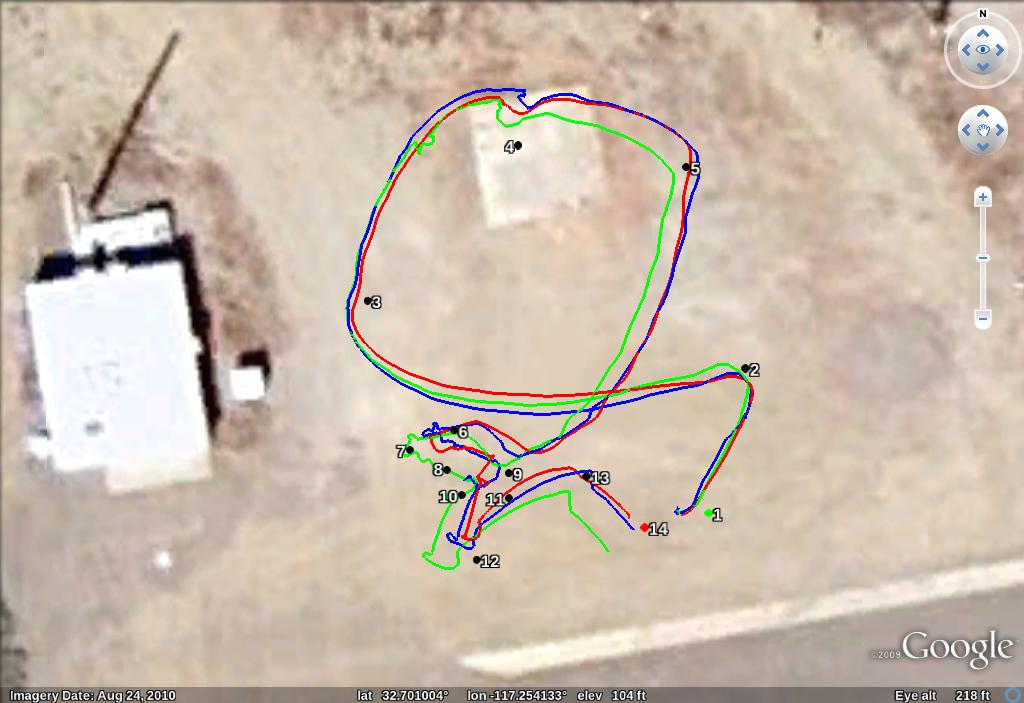
\includegraphics[width=.5\textwidth]{images/GE/20101203_1545_kf_lyapNewQR}
	\caption{Model Based Controller with Learned Noise Models}
	\label{fig:kfResults2}
\end{figure}

Model based with DGPS as input to Kalman filter and learned noise models.

\begin{figure}[ht!]
	\centering
	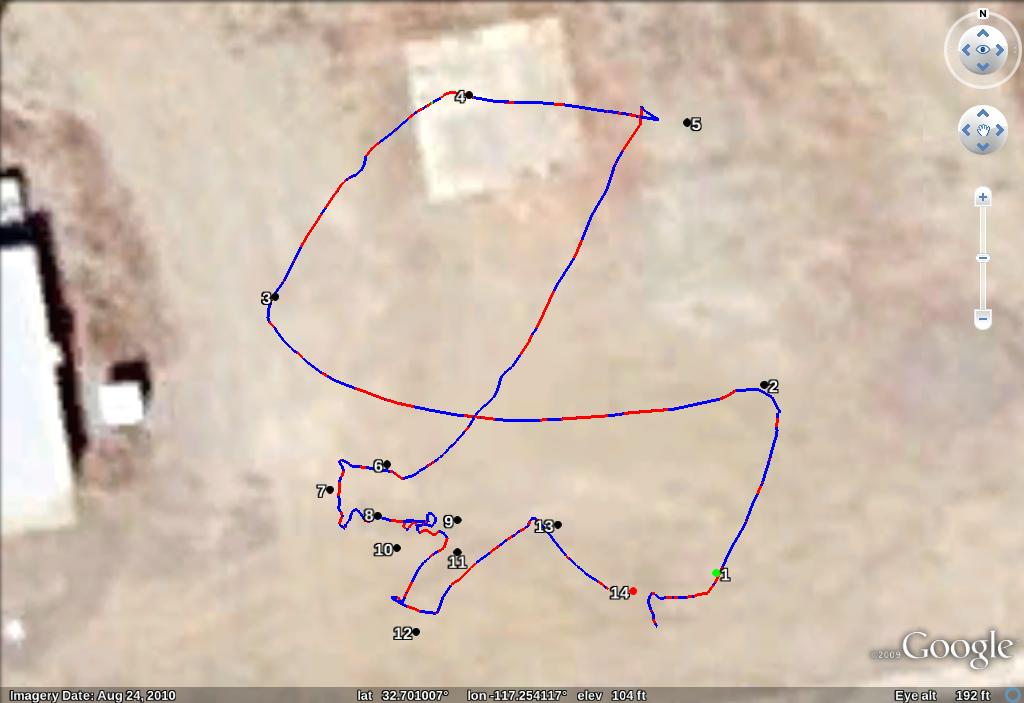
\includegraphics[width=.5\textwidth]{images/GE/20101203_1606_kf_lyapUsingDgpsNewQR}
	\caption{Model Based Controller with DGPS and Learned Noise Models}
	\label{fig:kfResults3}
\end{figure}

PID with original noise models.

\begin{figure}[ht!]
	\centering
	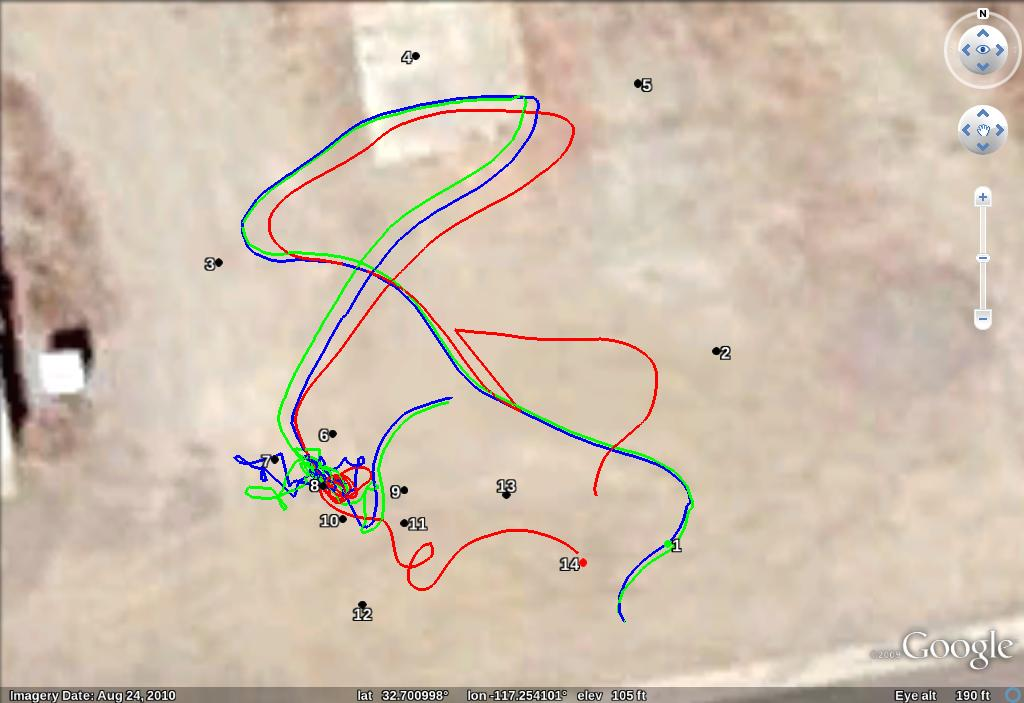
\includegraphics[width=.5\textwidth]{images/GE/20101203_1755_kf_pidOrigQR}
	\caption{PID Controller with Original Noise Models}
	\label{fig:kfResults4}
\end{figure}

PID with learned noise models.

\begin{figure}[ht!]
	\centering
	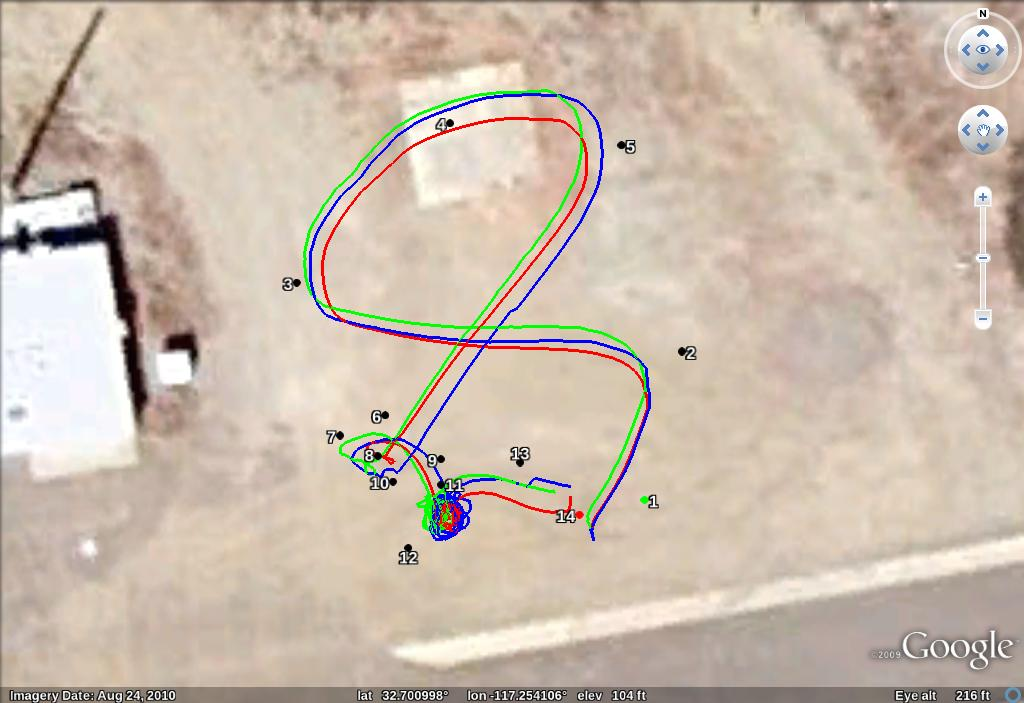
\includegraphics[width=.5\textwidth]{images/GE/20101203_1751_kf_pidNewQR}
	\caption{PID Controller with Learned Noise Models}
	\label{fig:kfResults5}
\end{figure}

PID with DGPS as input to Kalman filter and learned noise models.

\begin{figure}[ht!]
	\centering
	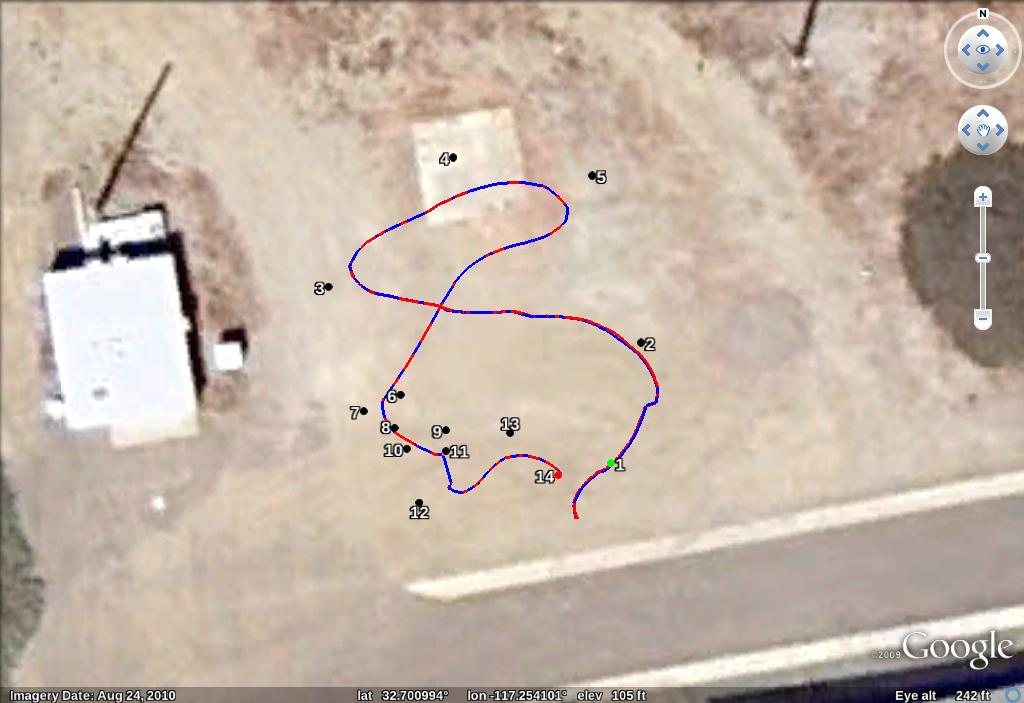
\includegraphics[width=.5\textwidth]{images/GE/20101203_1803_kf_pidUsingDgpsNewQR}
	\caption{PID Controller with DGPS and Learned Noise Models}
	\label{fig:kfResults6}
\end{figure}

\section{Model Based Controller Results}
\label{sec:lyapunovResults}
The control law derived in (\ref{eq:lyapunovControlLaw}) was tested in the previously described area in two different ways. The first set of results used a single set of gains and had the goal heading set to use the current heading of the robot so that $\theta^\star=\alpha$ as discussed in Chapter \ref{sec:lyapunovVariables}. Figure *** shows the actual position of the robot during navigation as well as the waypoints that defined the desired route.

Figures \ref{fig:resultsLyapunov1} - \ref{fig:resultsLyapunov6} shows how the linear and angular velocities changed over time as measured by the Kalman filter output. The gains used were $h=0.1$, $k=0.25$ and $\gamma=0.23$. A clear deceleration can be seen as the robot approaches each waypoint although the linear velocity does not go to zero until the final waypoint due to the use of the carrot in the path planner as discussed in Chapter \ref{sec:lyapunovVariables} for determing the error distance $e$. One of the consequences of using a model based controller is that a negative linear velocity was used after reaching the second waypoint and having the error angle $\alpha$ move towards the third waypoint which is rarely, if ever, encountered when using the original PID controller.

\begin{figure}[ht!]
	\centering
	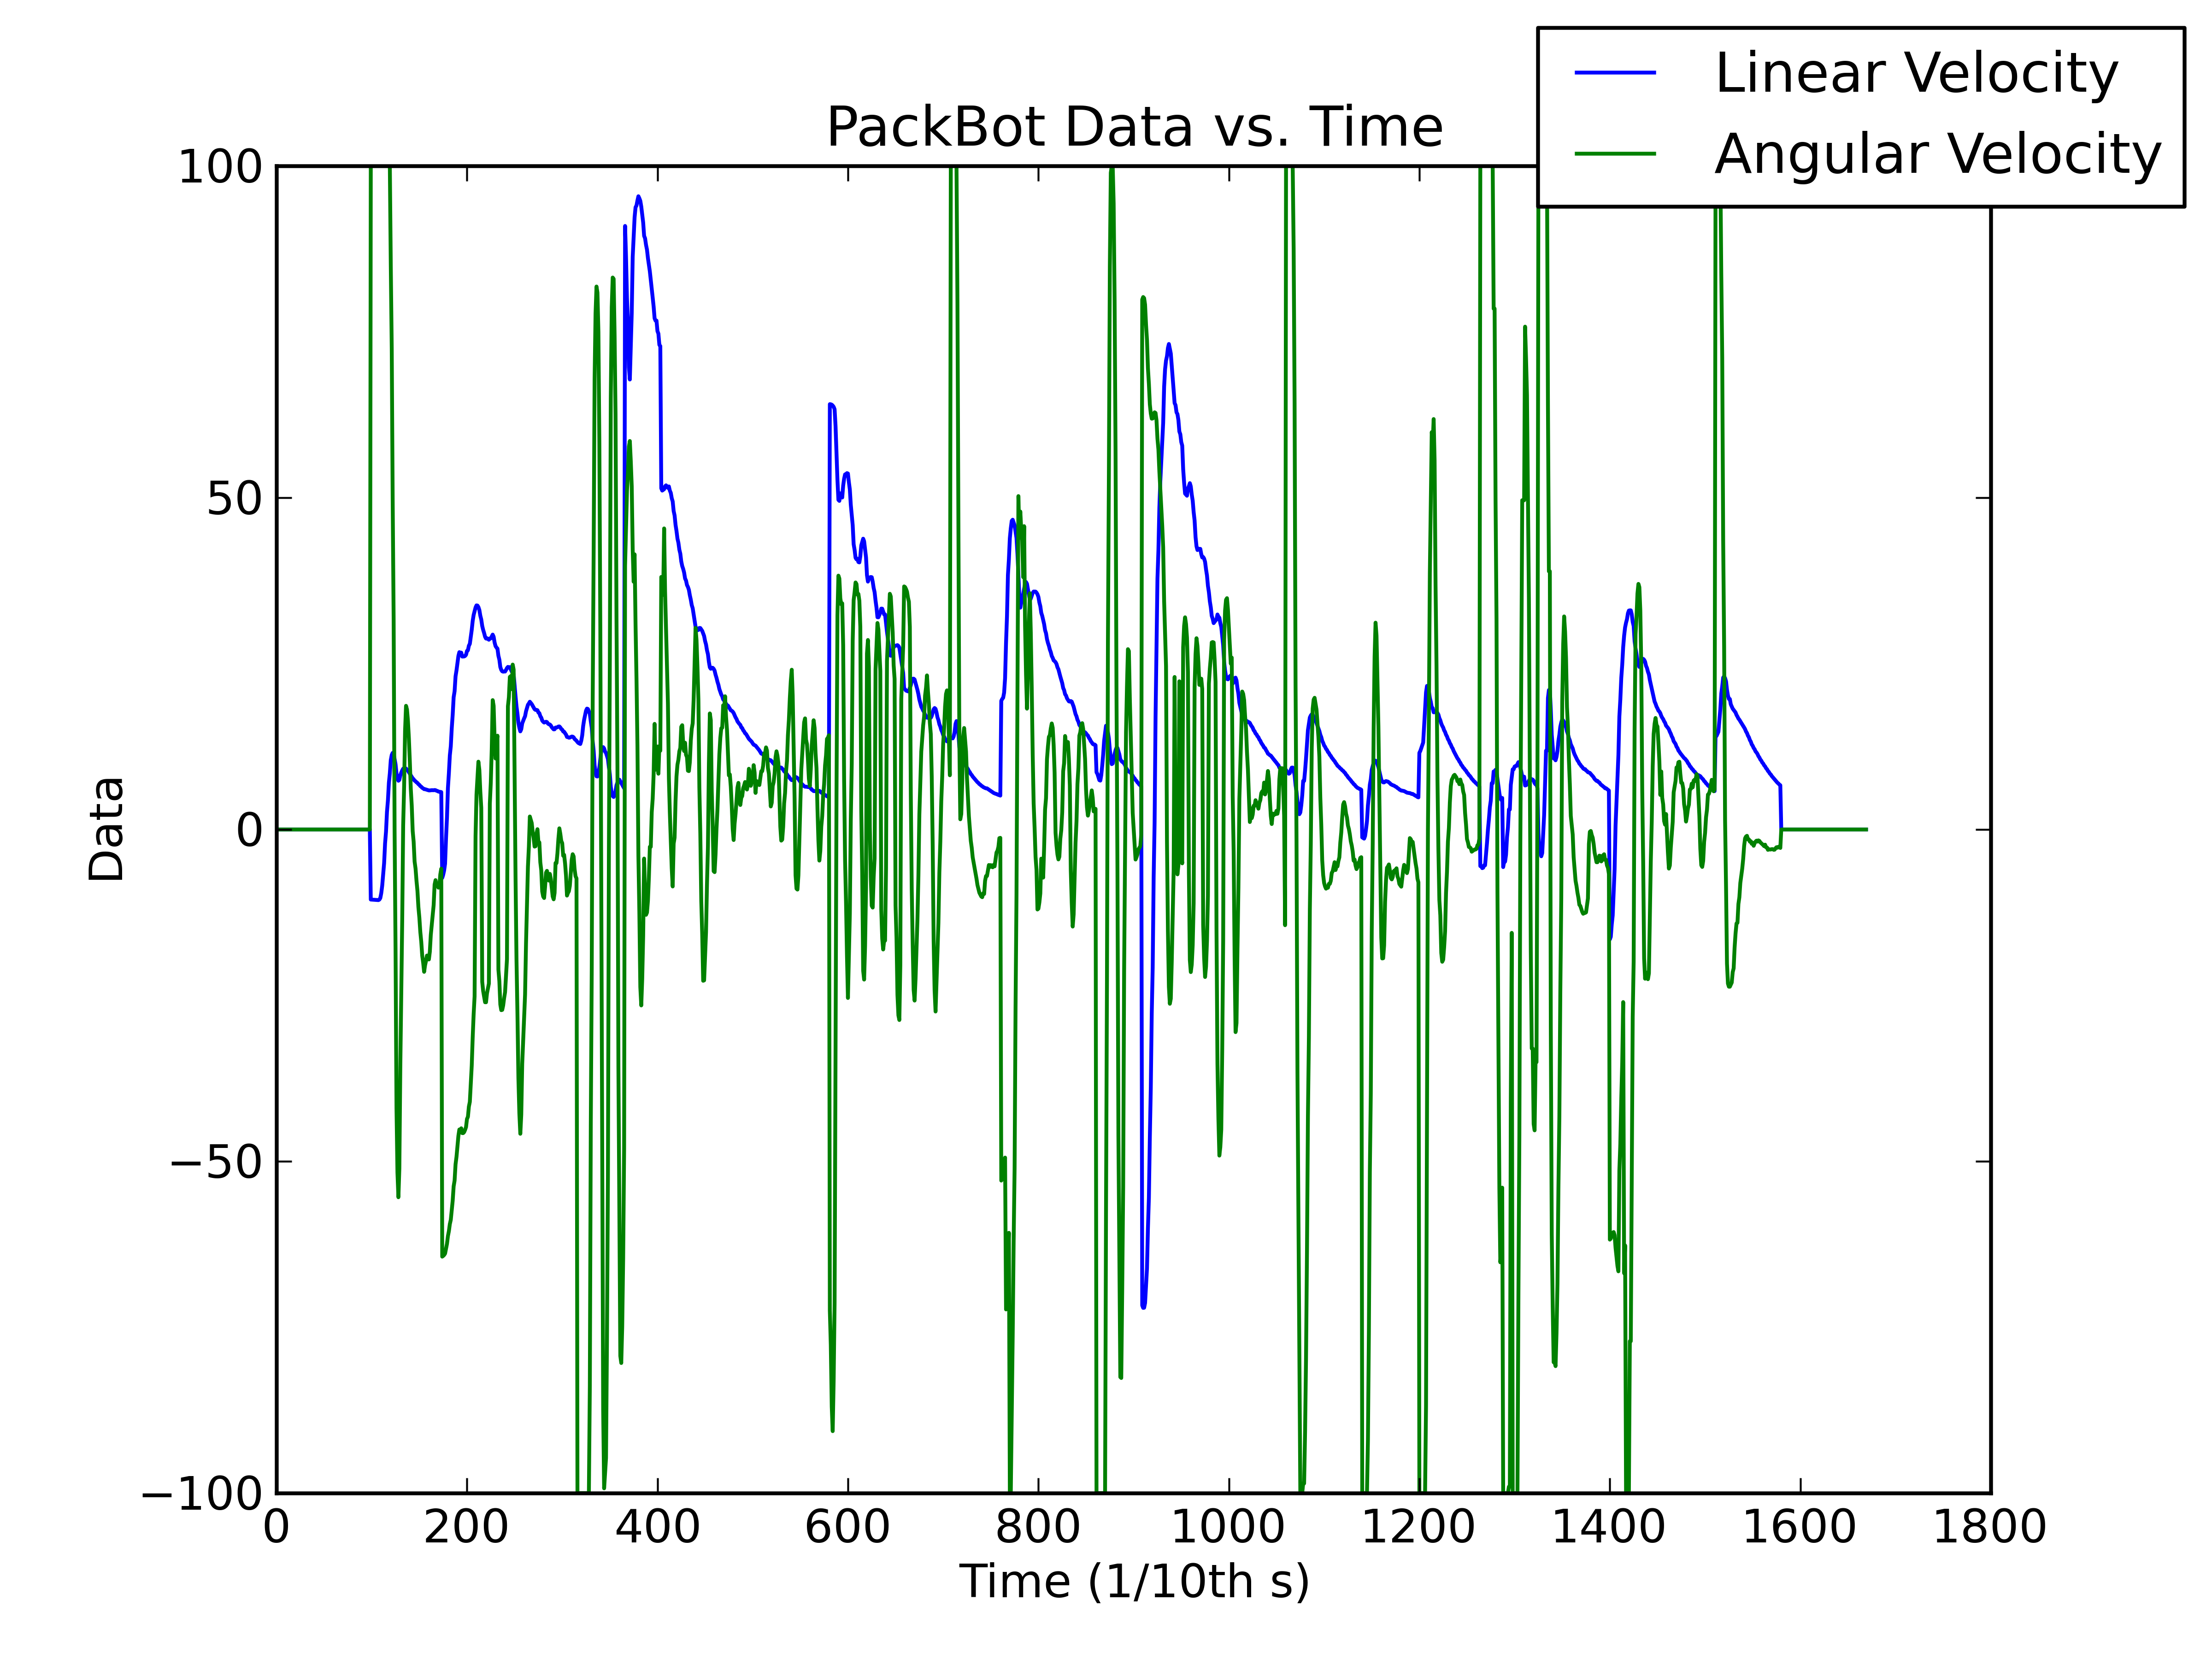
\includegraphics[width=.5\textwidth]{images/pbtx/20101203_1551_pbtxLyapOrigQR}
	\caption{Model Based Controller with Original Noise Models}
	\label{fig:resultsLyapunov1}
\end{figure}

\begin{figure}[ht!]
	\centering
	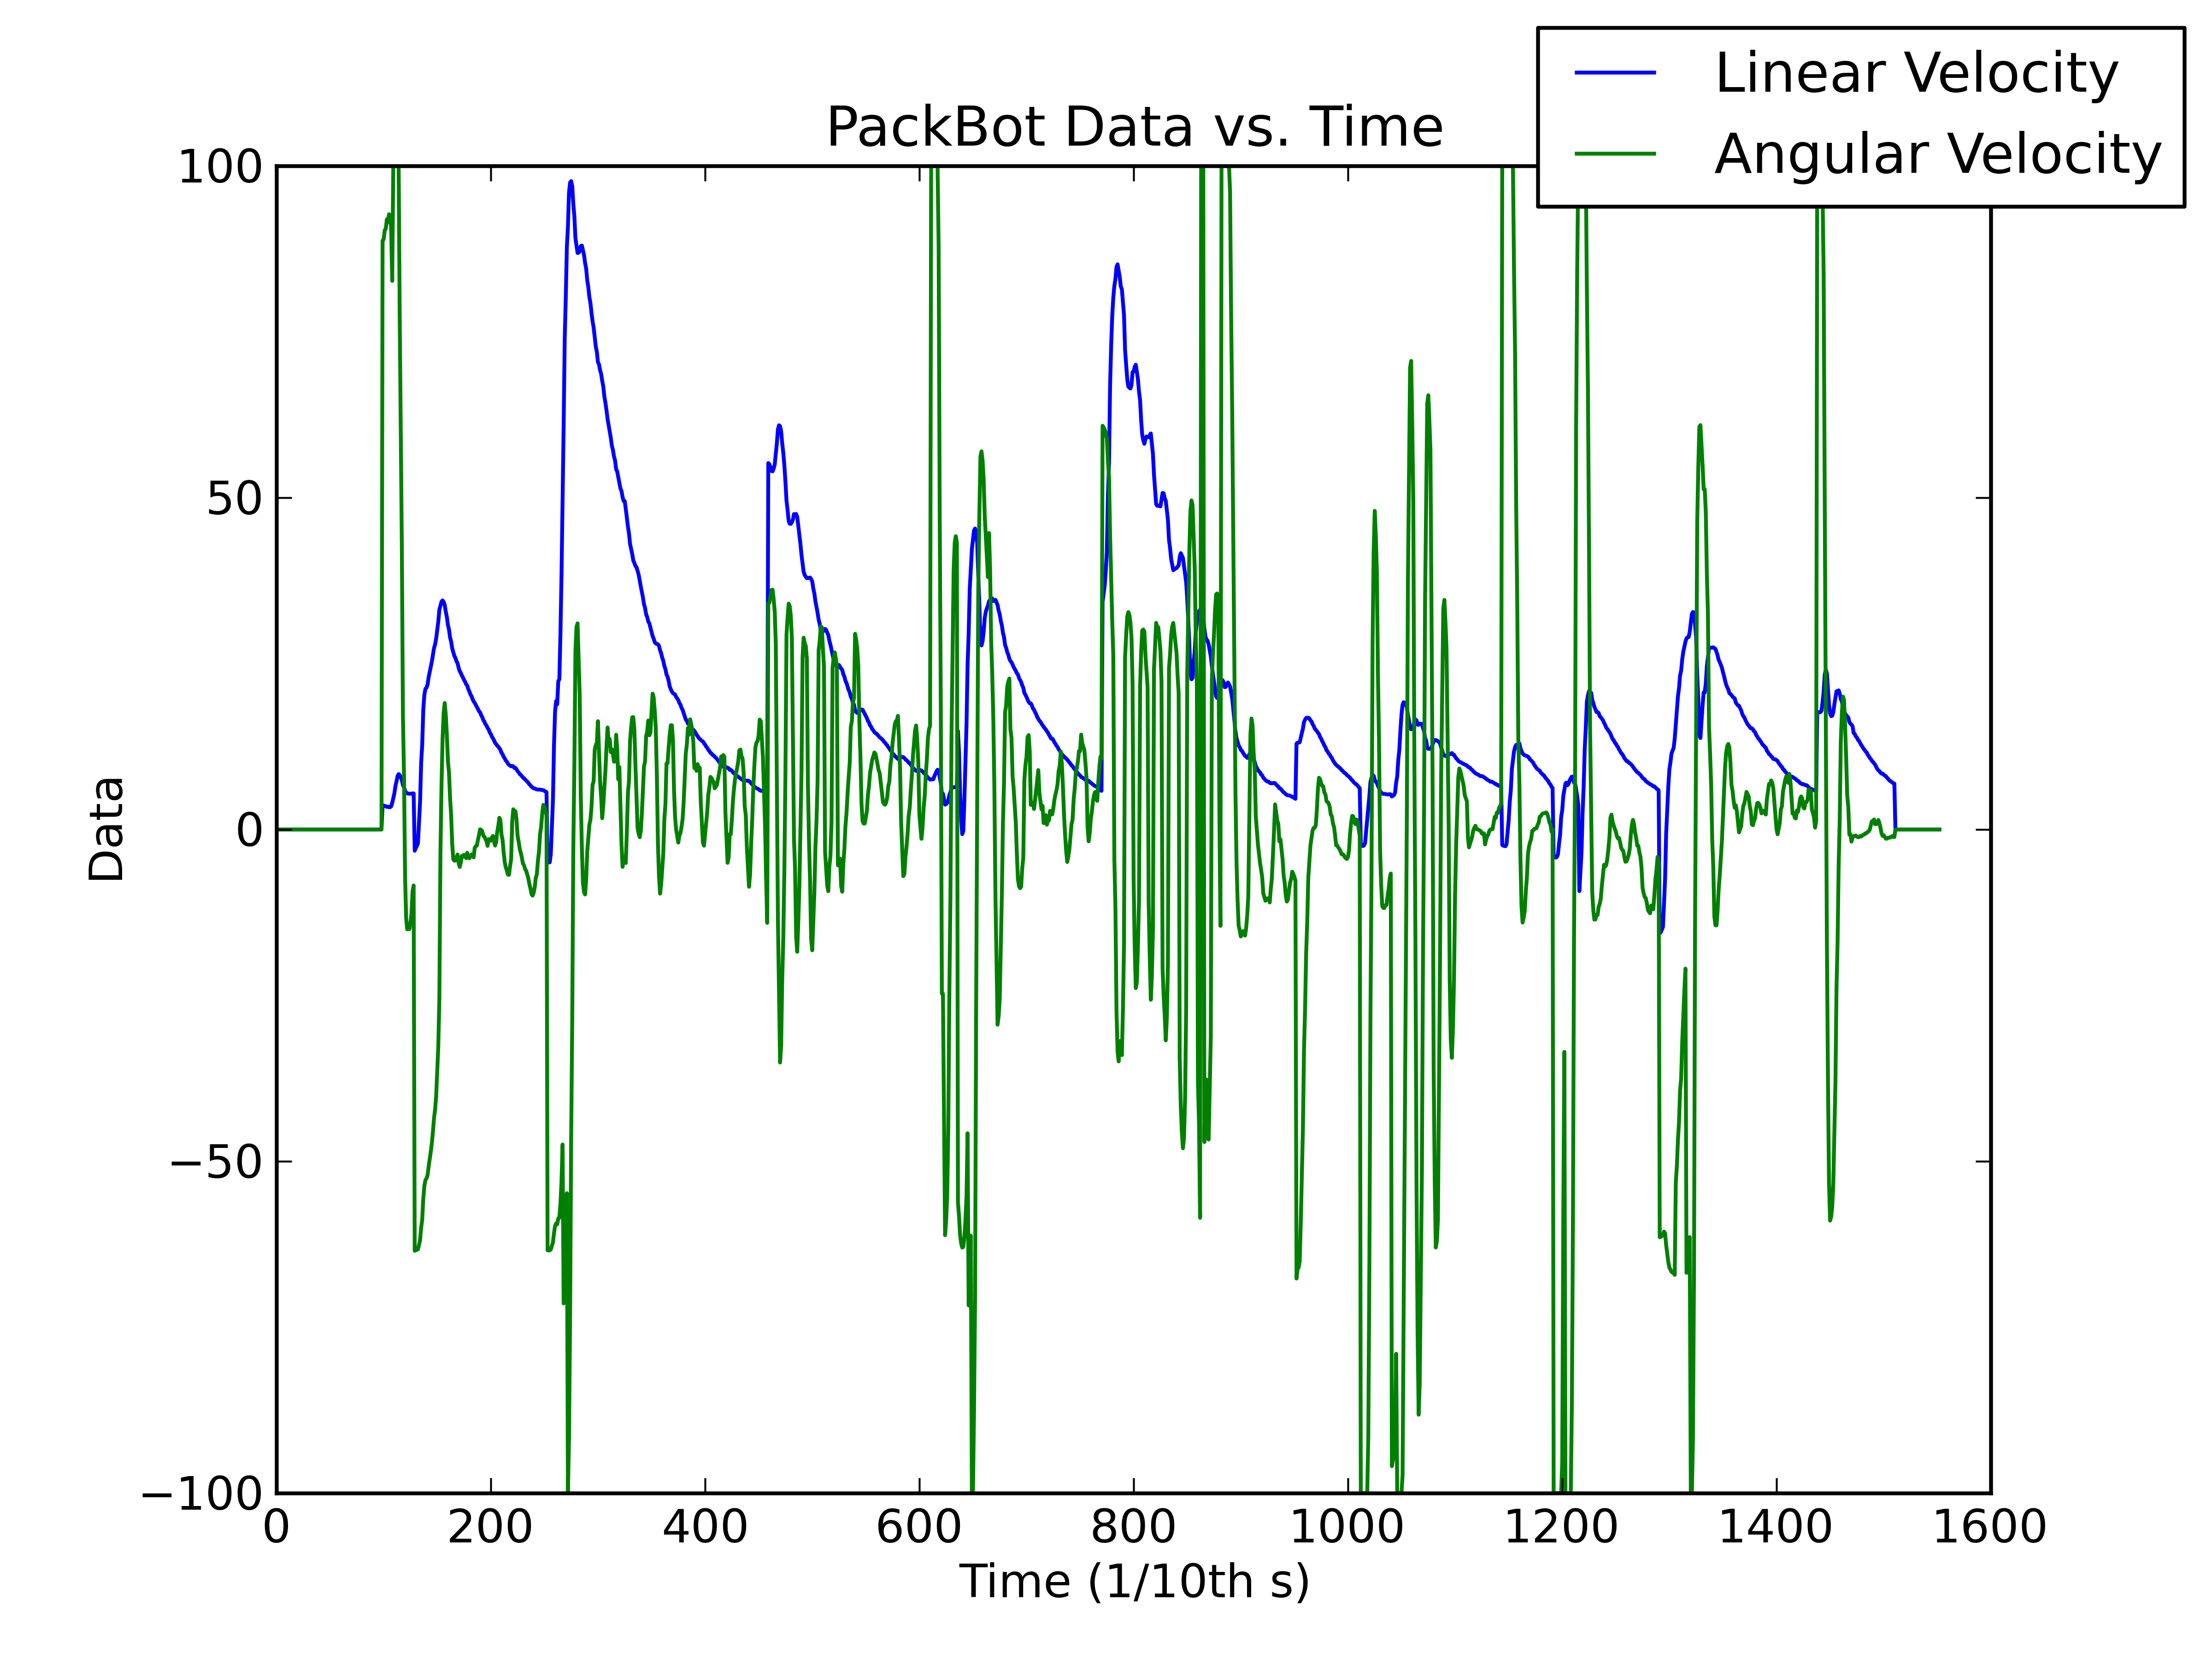
\includegraphics[width=.5\textwidth]{images/pbtx/20101203_1545_pbtxLyapNewQR}
	\caption{Model Based Controller with Learned Noise Models}
	\label{fig:resultsLyapunov2}
\end{figure}

\begin{figure}[ht!]
	\centering
	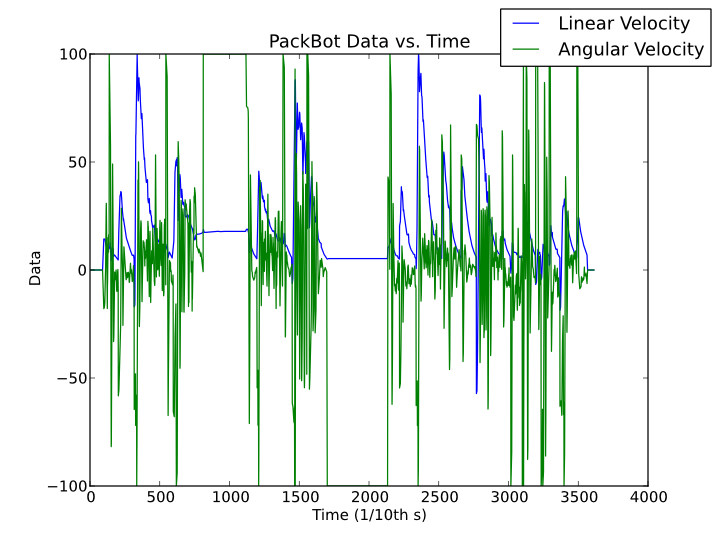
\includegraphics[width=.5\textwidth]{images/pbtx/20101203_1606_pbtxLyapUsingDgpsNewQR}
	\caption{Model Based Controller Using DGPS with Learned Noise Models}
	\label{fig:resultsLyapunov3}
\end{figure}

\begin{figure}[ht!]
	\centering
	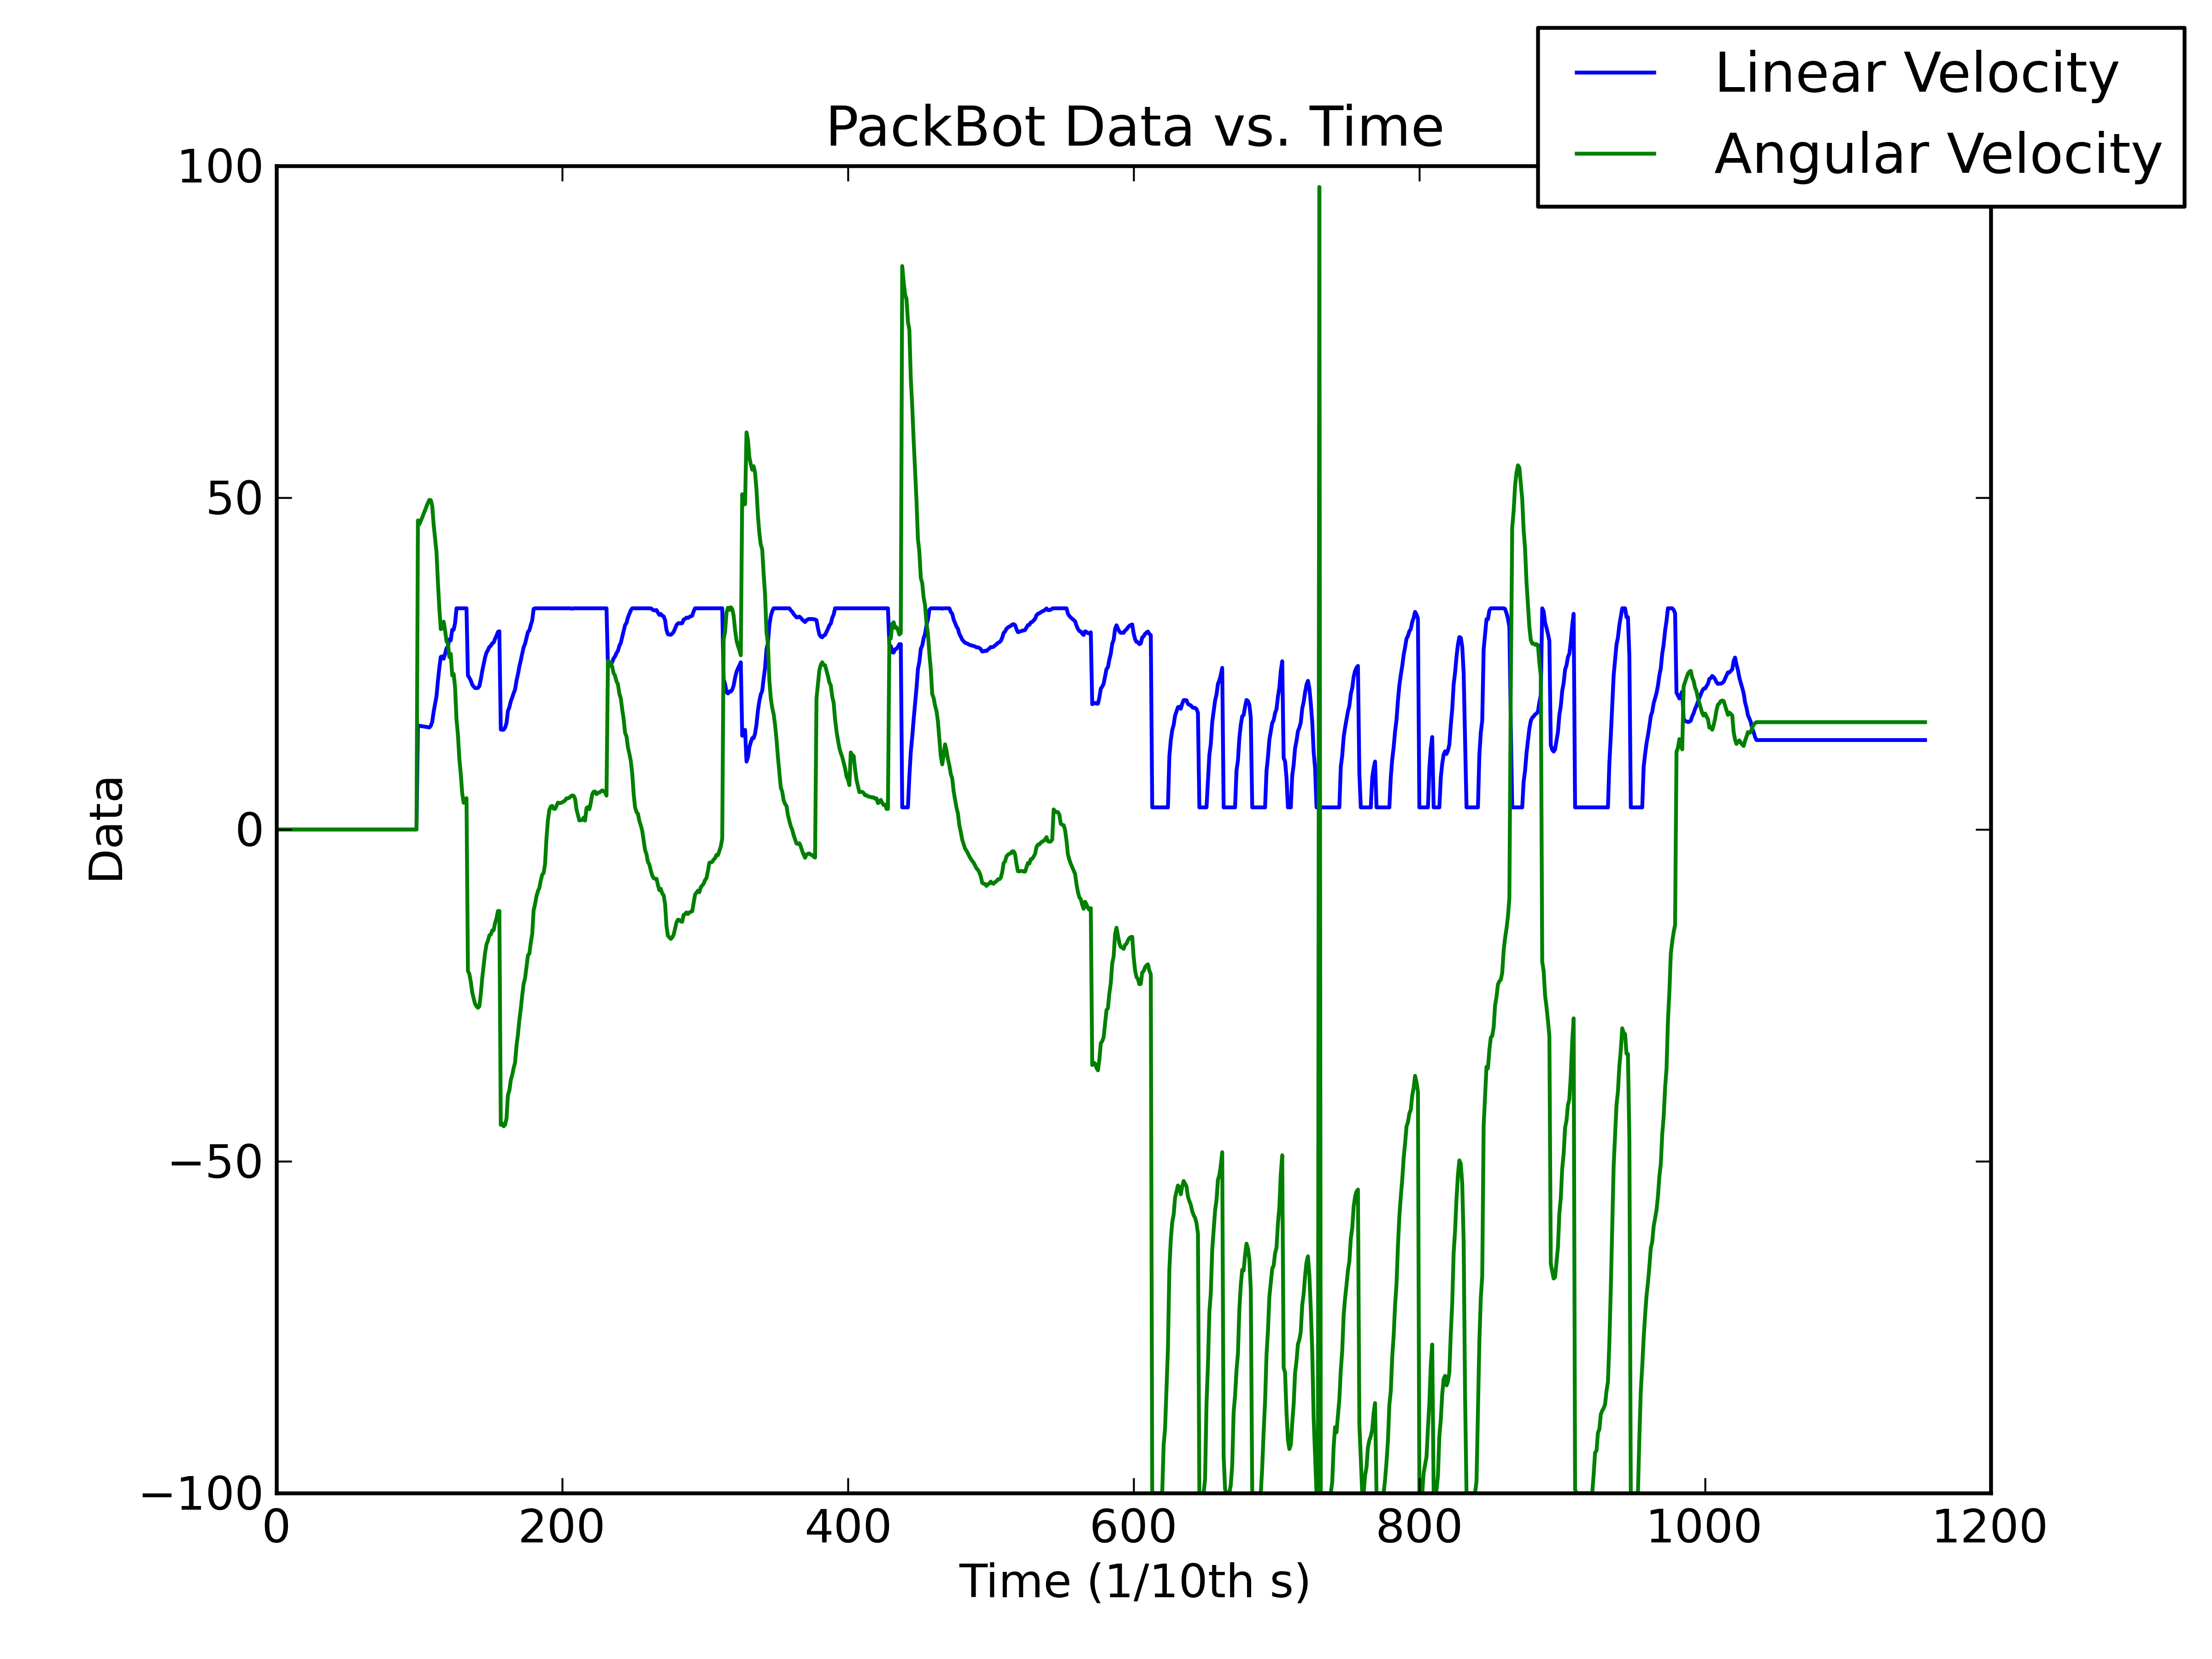
\includegraphics[width=.5\textwidth]{images/pbtx/20101203_1755_pbtxPidOrigQR}
	\caption{PID Controller with Original Noise Models}
	\label{fig:resultsLyapunov4}
\end{figure}

\begin{figure}[ht!]
	\centering
	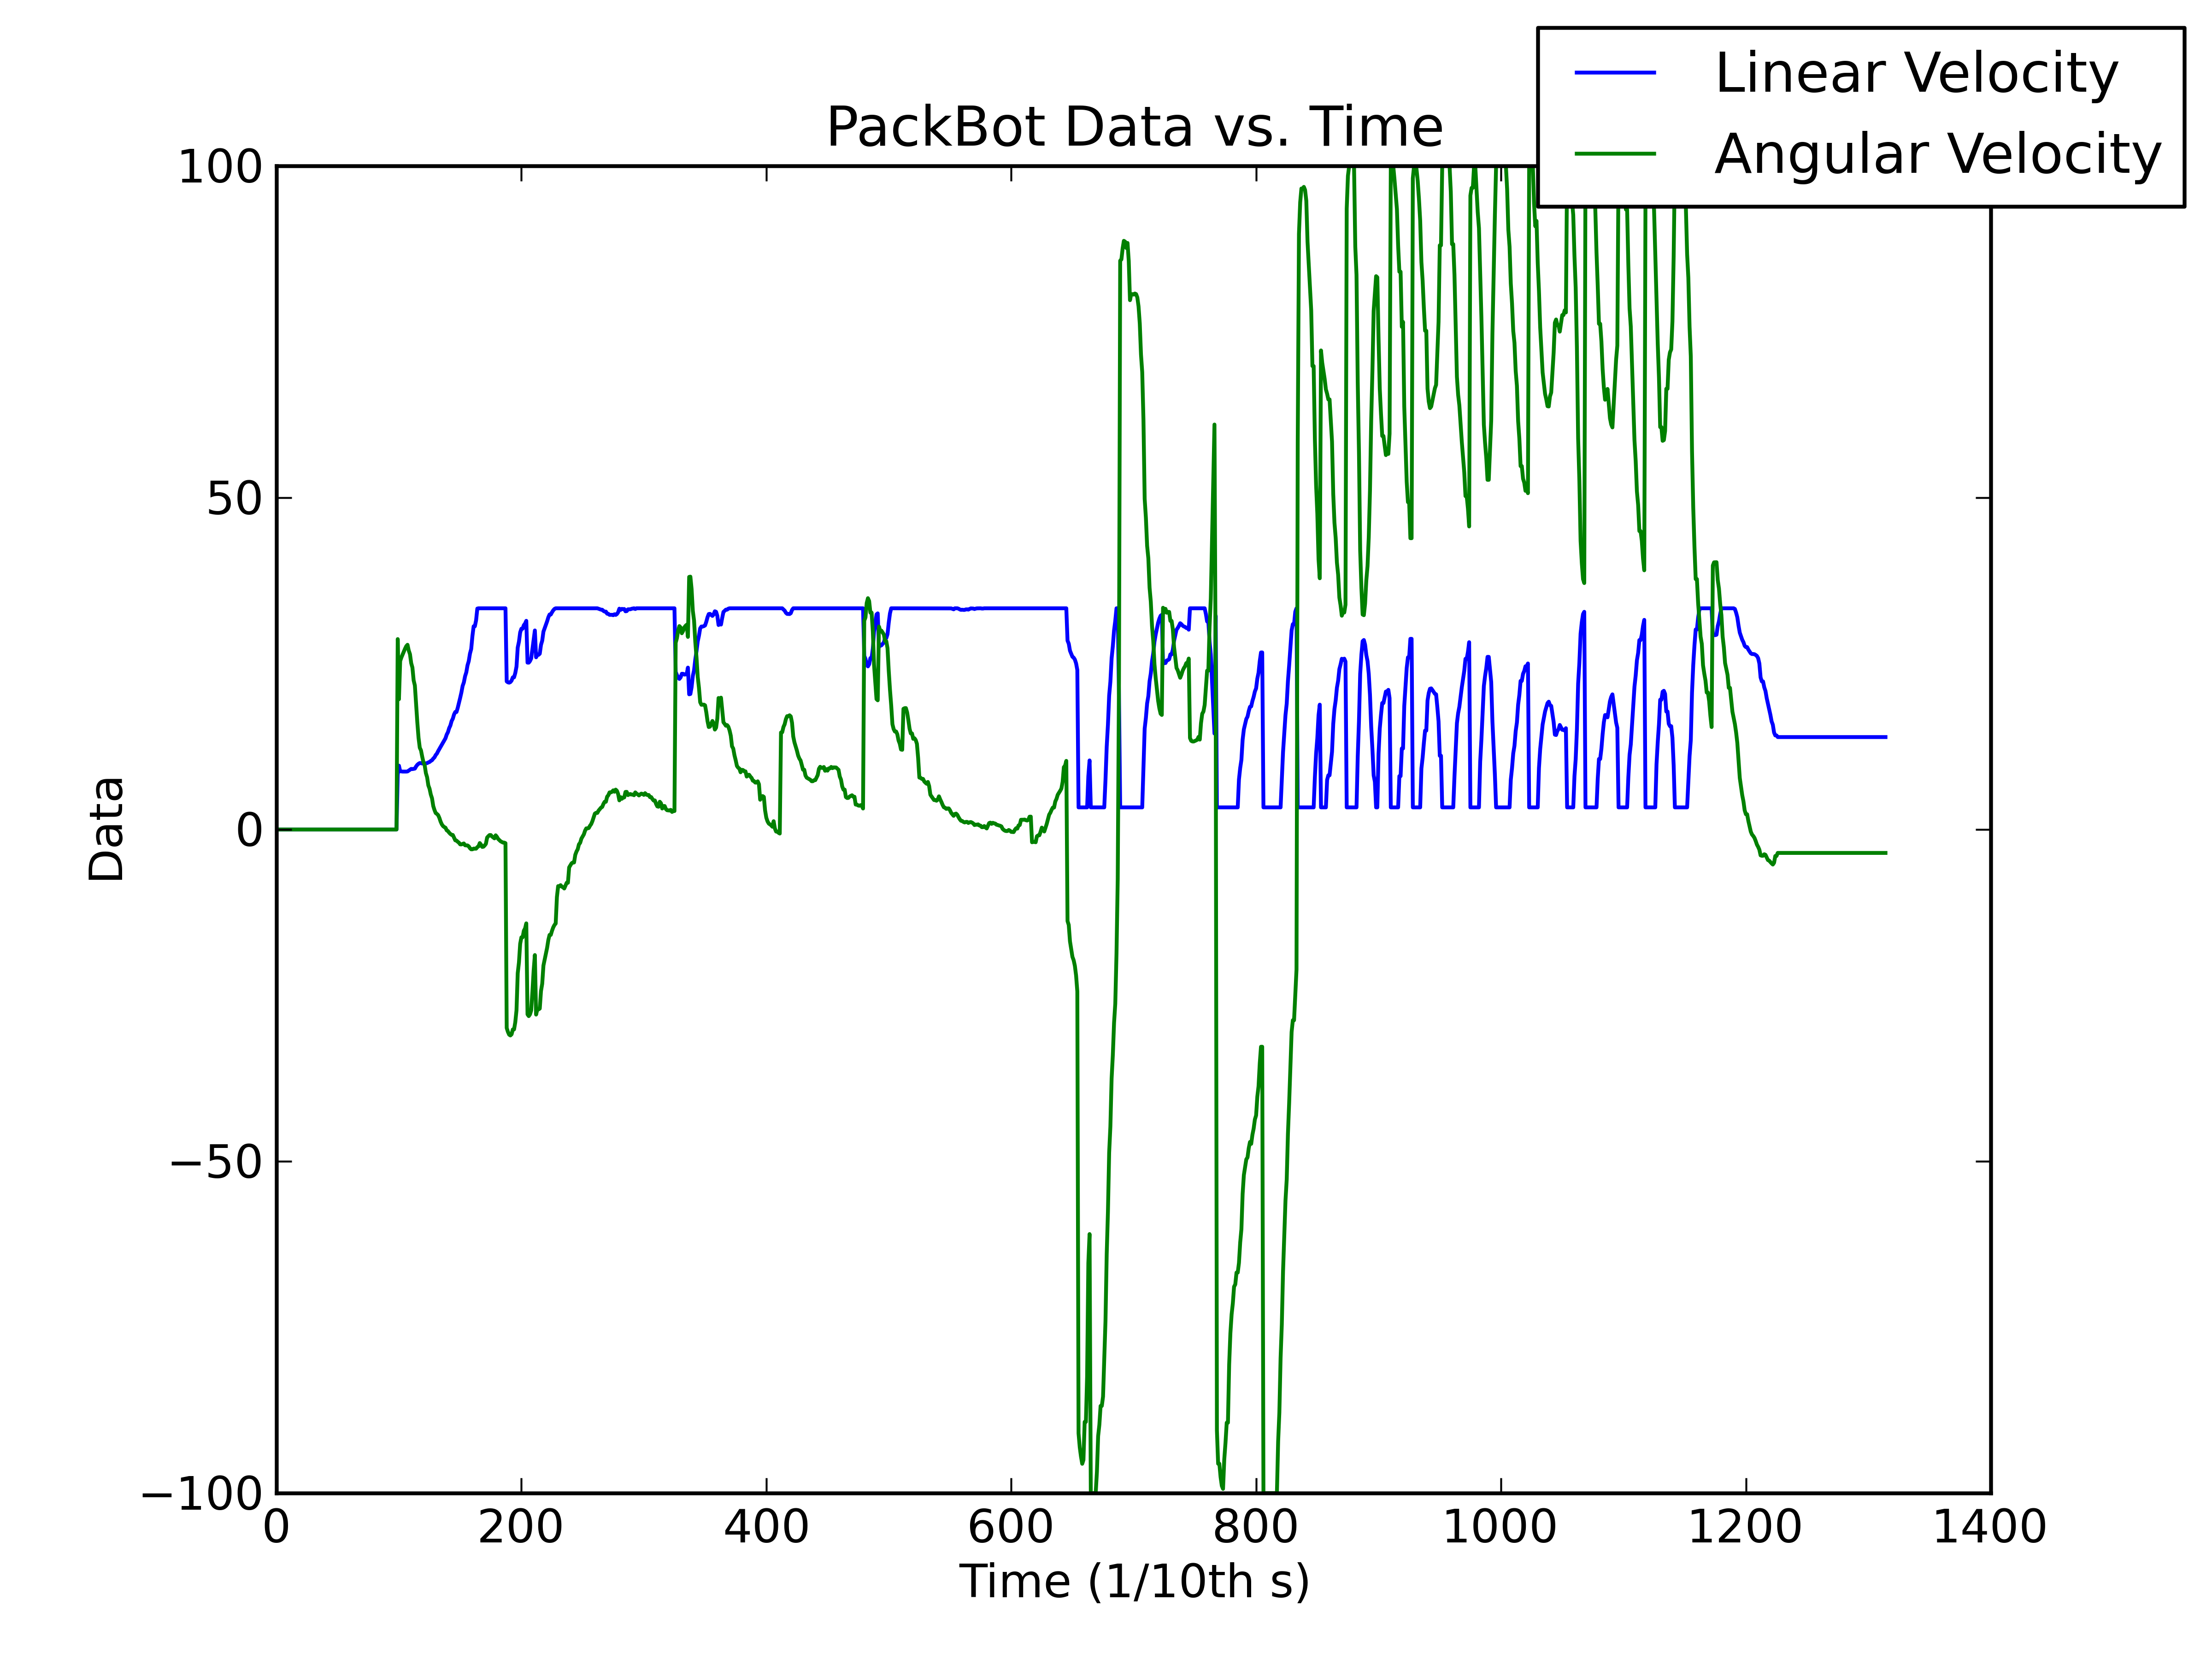
\includegraphics[width=.5\textwidth]{images/pbtx/20101203_1751_pbtxPidNewQR}
	\caption{PID Controller with Learned Noise Models}
	\label{fig:resultsLyapunov5}
\end{figure}

\begin{figure}[ht!]
	\centering
	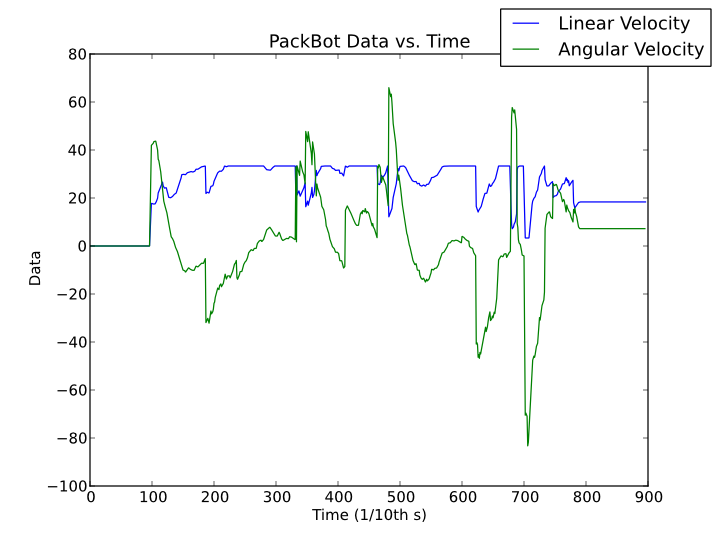
\includegraphics[width=.5\textwidth]{images/pbtx/20101203_1803_pbtxPidUsingDgpsNewQR}
	\caption{PID Controller Using DGPS with Learned Noise Models}
	\label{fig:resultsLyapunov6}
\end{figure}

The process of selecting gains in Chapter \ref{sec:lyapunovTrajectoryConvergence} only applies as $(\alpha, \theta)\to(0,0)$ but says nothing about what happens when the angle errors are not small. Empirically it was determined that the gains $h=0.25$, $k=0.2$ and $\gamma=0.2$ worked well in creating smooth trajectories and later it was found that these gains cause $\zeta=1$ so that, when the angle errors are small, the system $A$ is critically damped although $\sigma>\gamma$ so the distance error converges faster than the angle errors. The best results occurred when the gains were set to $h=0.25$, $k=0.2$ and $\gamma=0.2$ \textit{until} the angle errors were $|\alpha|<0.5$ \textit{and} $|\theta|<0.5$ radians which leads to the linear approximation being valid and the gains were then changed to $h=1.1$, $k=0.42$ and $\gamma=0.2$. This second set of gains, used when the angle errors were small, are critically damped for the system $A$ since $\zeta=1$ and the angle errors converge faster than the distance error since $\sigma>\gamma$. The results of this adaptive gain scheme can be seen in Figures \ref{fig:resultsLyapunovPositionAdaptive} and \ref{fig:resultsLyapunovVelocitiesAdaptive}. Note that the goal heading, $\theta^\star$, was set to be the angle from the current waypoint to the next waypoint so that the robot would be pointing in the direction of the next waypoint when it reached the current waypoint. For the last waypoint in the route the goal heading used was $\theta^\star=\alpha$.

\begin{figure}[ht!]
	\centering
	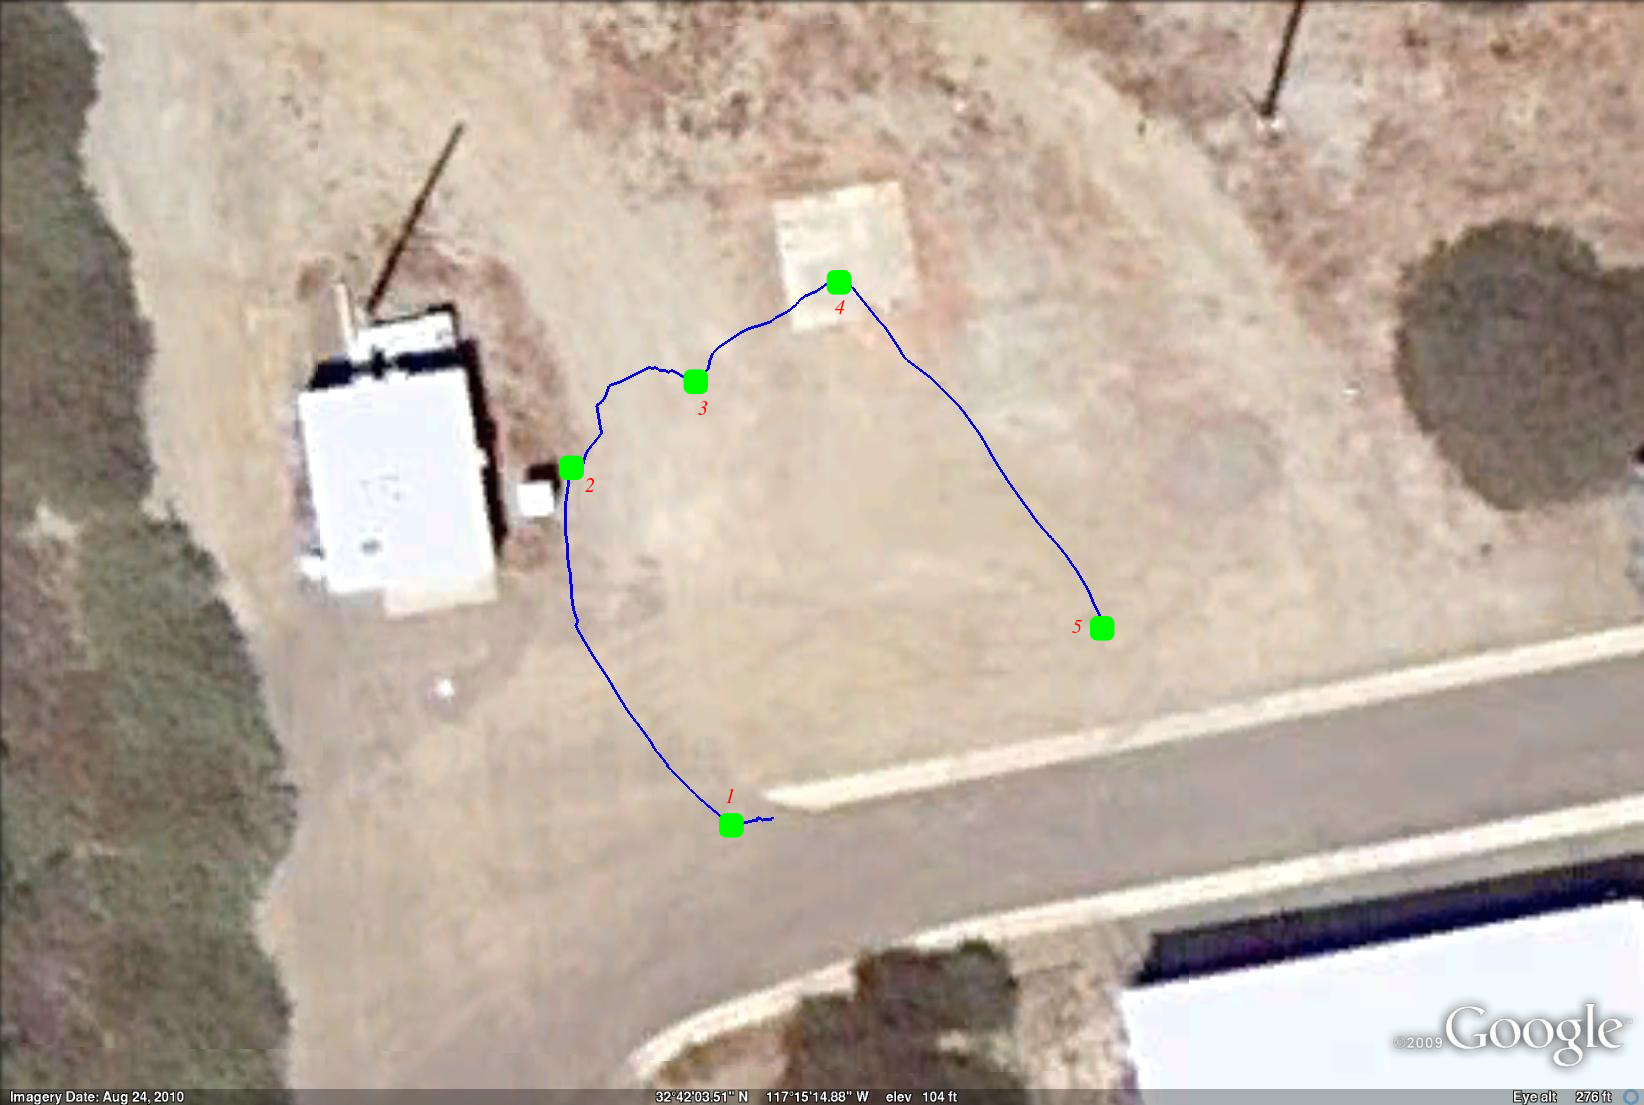
\includegraphics[width=.5\textwidth]{images/20100929_1448_GE_KF_waypts}
	\caption{Robot Position using Adaptive Gain Scheme}
	\label{fig:resultsLyapunovPositionAdaptive}
\end{figure}

\begin{figure}[ht!]
	\centering
	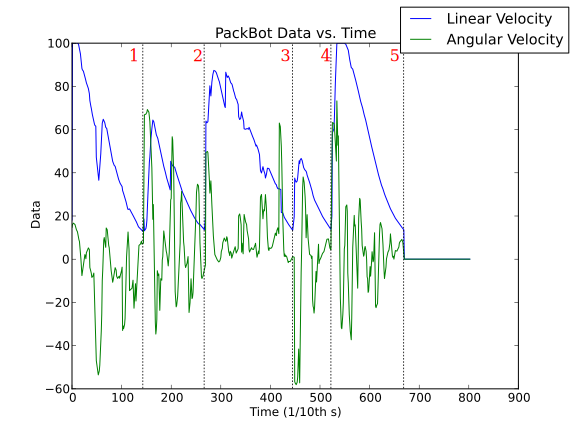
\includegraphics[width=.5\textwidth]{images/20100929_1448_pbtx}
	\caption{Linear and Angular Velocities with Adaptive Gain Scheme}
	\label{fig:resultsLyapunovVelocitiesAdaptive}
\end{figure}

\subsection{Controller Comparison}
\label{sec:controllerComparison}
For both PID (Chapter \ref{sec:pid}, Table \ref{tab:PIDGainEffects}) and the model based controller (Chapter \ref{sec:lyapunovTrajectoryConvergence}) gains have to be selected, the difference being that stability is the goal when selecting PID gains whereas stability is guaranteed with the model based controller. More advanced behaviors such as three point turns are a consequence of the control law in (\ref{eq:lyapunovControlLaw}) derived using a kinematic model of the robot. The other very large difference between the controllers is that a table of gains must be tuned for the PID controller to work at varying linear velocities but the model based controller works very well at different linear and angular velocities. Also, when properties of the robot such as mass are changed by using different payloads for the system the entire table of PID gains must be retuned while, at most, one set of gains must be retuned for the model based controller. This last benefit of the model based controller makes it very appealing to use in fielded systems since it reduces the amount of maintenance and effort required to keep the robot in working condition. The model based controller will also allow for improved navigation performance near obstacles which leads directly to improved autonomy for the robot.

\chapter{Future Work}
\label{ch:futurework}

\begin{itemize}
\item Use the results from this work to make retrotraverse work better. One way this can be accomplished is that obstacles should be easier to avoid since the robot position is more accurate so following a previously navigated path after some time has passed should result in less drift so previously avoided static obstacles will be closer to where they were before. Additionally, a control law that works at varying speeds (like model based, unlike PID that had to be tuned with different gains for different speeds) will make navigation around obstacles smoother and faster.
\item Work on a planner that can automatically tune the gains for the model based controller based on the environment of the robot. For example, if there are no nearby obstacles then let the path curvature be large. If the environment is cluttered then force the path curvature to be much smaller. Similarly, a planner that can select the best controller out of PID, fuzzy logic and model based would likely improve the navigation characteristics of the robots.
\item Use the learning algorithm for indoor robots as there is no reason why a robot needs to have GPS to benefit from using the DGPS system for training the $Q$ and $R$ matrices in the EKF. A test area would need to be set up outdoors so that DGPS can be used and the normal sensors also work by bouncing off walls and what not but the DGPS ground truth position can be converted to the local coordinate system and used to generate an error metric for the EKF position output.
\item Use a high quality IMU and compass that serve as ground truth for Euler angles in addition to the DGPS system so that the training algorithm attempts to minimize the errors between Euler angles in addition to position.
\item Implement the more advanced work done by \cite{Lapierre06} and \cite{Gulati08} to improve the performance of the model based controller. In particular \cite{Gulati08} uses control Lyapunov functions that attempt to constrain the accelerations of the vehicle and uses splines to generate intermediate waypoints between the vehicles current position and the goal position.
\item Extend the model based controller to have constraints that allow the controller to work with non-unicycle like vehicles such as those that have Ackerman steering like most personal automobiles which are not physically able to rotate in place.
\item Build on the current extended Kalman filter in ACS to implement an unscented Kalman filter as described by \cite{ThrunProbRobots06} to better handle the nonlinearities of the system.
\end{itemize}

\chapter{Conclusion}
\label{ch:conclusion}
As shown in Chapter \ref{ch:results}, the estimation and controls algorithms developed and implemented as part of this thesis resulted in significant improvements to the existing algorithms used for EOD robots. The Kalman filter showed a significant improvement over initial results. The model-based controller was shown to drive at multiple velocities, across different surfaces, with no gain tuning required. This is contrary to the original PID controller. Additionally, the model-based controller exhibits smooth deceleration as it approaches waypoints, which is a consequence of the control law and not due to external commands to slow down like the PID controller. These improvements to robot navigation have been implemented in ACS and are now running on fielded systems to the benefit of end users.

There now exist better answers to the questions of "Where am I?" and "How do I get there?" due to the results obtained in this thesis.

% \appendix % Use \appendix for single, \appendices for multiple
% \chapter{Source Code}
\label{ch:code}
This is some of the source code used in this research. Contact the \mailto{\thesisAuthorEmail}{author} for more complete listings.

\section{QR}
\label{sec:qrcode}
This code was used to generate the $Q$ and $R$ matrices.
% Set the syntax highlighting to C++.
\lstset{language=C++}
\matlabscript{code/qr/qr.cc}{C++ source file for genearating $Q$ and $R$ matrices.}
\matlabscript{code/qr/qr.h}{C++ header file for genearating $Q$ and $R$ matrices.}
\matlabscript{code/qr/metrics.cc}{C++ source file for calculating errors.}

\clearpage
\section{DGPS}
\label{sec:dgpscode}
This code was used to set up and communicate with DGPS receivers.
\matlabscript{code/gpslogger/gpslogger.cpp}{Main C/C++ file for logging GPS data.}
% \matlabscript{code/gpslogger/oem4.cpp}{Main C++ file for the Novatel OEM4 library.}

\clearpage
\section{Lyapunov}
\label{sec:lyapunovcode}
This code was adapted from \cite{Rusu05RobotuxLyapunov}. Most of the changes involved making the code more efficient, making it easier to modify the parameters and variables, adding additional comments and using more descriptive variable names.
% Set the syntax highlighting back to Matlab.
\lstset{language=Matlab}
\matlabscript{code/lyapunovRusu/main.m}{Main Matlab file for Lyapunov controller.}
\matlabscript{code/lyapunovRusu/f3.m}{Matlab file for ODE solver for Lyapunov controller.}
\matlabscript{code/lyapunovRusu/CalcETA.m}{Matlab file for calculating the robot trajectory for Lyapunov controller.}

% \chapter{List of Acronyms}%
\label{ch:acronyms}
*** Put a list of acronyms here. ***


% Bibliography.
\bibliographystyle{these}
% \bibliographystyle{plain}
\bibliography{mybib}

\end{document}
